%!TEX program = xelatex
\documentclass[11pt,a4paper]{article}
\usepackage[utf8]{inputenc}
\usepackage[T1]{fontenc}
\usepackage{authblk}
\usepackage{ctex}
\usepackage{tikz}
\usepackage{pgfplots}
\usepackage{verbatim}
\usepackage{amsfonts}
\usepackage{amsmath}
\usepackage{amsthm}
\usepackage{indentfirst}
\usepackage{amssymb}
\setlength{\parindent}{0pt}
\usetikzlibrary{shapes,snakes}
\newcommand{\argmax}{\operatornamewithlimits{argmax}}
\newcommand{\argmin}{\operatornamewithlimits{argmin}}
\DeclareMathOperator{\col}{col}
\usepackage{booktabs}
\newtheorem{theorem}{Theorem}
\newtheorem{note}{Note}
\newtheorem{definition}{Definition}
\newtheorem{proposition}{Proposition}
\newtheorem{lemma}{Lemma}
\newtheorem{example}{Example}
\newtheorem{corollary}{Corollary}
\usepackage{graphicx}
\usepackage{geometry}
\usepackage{hyperref}
\newcommand{\code}{	exttt}
\geometry{a4paper,scale=0.8}
\title{STAT 425 Note 汇总}
\author[*]{Wenxiao Yang}
\affil[*]{Department of Mathematics, University of Illinois at Urbana-Champaign}
\date{2021}

\usepackage{listings}
\usepackage{xcolor}

\lstset{numbers=left,numberstyle=\tiny,keywordstyle=\color{blue},commentstyle=\color[cmyk]{1,0,1,0},frame=single,escapeinside=``,extendedchars=false,xleftmargin=2em,xrightmargin=2em,aboveskip=1em,tabsize=4,showspaces=false}






\begin{document}
\maketitle
\tableofcontents
\newpage


\section{Review of statistics}
\subsection{Random Vectors}
\subsubsection{Mean}
$$\mu =\mathbb{E}(\mathbf{Z})=\begin{pmatrix}
    \mathbb{E}(Z_1)\\
    \mathbb{E}(Z_2)\\
    \cdots\\
    \mathbb{E}(Z_m)
\end{pmatrix}$$
\subsubsection{Variance-Covariance matrix $\Sigma$}
$$\Sigma_{m\times m}=Cov(\mathbf{Z})=\mathbb{E}((\mathbf{Z}-\mu)(\mathbf{Z}-\mu)^T)=\begin{bmatrix}
    Var(Z_1)&\cdots	&Cov(Z_1,Z_m)\\
    \cdots&\cdots	&\cdots\\
    Cov(Z_m,Z_1)&\cdots &Var(Z_m)
\end{bmatrix}$$
\subsection{Affine Transformation}
(1)
$$\mathbf{W}=\mathbf{a}_{n\times 1}+\mathbf{B}_{n\times m}\mathbf{Z}_{m\times 1}$$
$$\mathbb{E}(\mathbf{W})=\mathbf{a}+\mathbf{B}\mu,\ Cov(\mathbf{W})=\mathbf{B}\Sigma \mathbf{B}^T$$
(2)
$$\mathbf{W}=\mathbf{v}^T \mathbf{Z}=v_1Z_1+...+v_mZ_m$$
$$\mathbb{E}(\mathbf{W})=\mathbf{v}^T\mu=\sum_{i=1}^mv_i\mu_i$$ $$Var(\mathbf{W})=\mathbf{v}^T\Sigma \mathbf{v}=\sum_{i=1}^mv_i^2Var(Z_i)+2\sum_{i<j}v_iv_jCov(Z_i,Z_j)$$
$$\text{i.e. }\mathbb{E}(\mathbf{A}\mathbf{Z})=\mathbf{A}\mathbb{E}(Z);\ Var(\mathbf{A}\mathbf{Z})=\mathbf{A}Var(\mathbf{Z})\mathbf{A}^T$$
(3)
$$Cov(\mathbf{A}\mathbf{X},\mathbf{B}\mathbf{Y})=\mathbb{E}[(\mathbf{A}\mathbf{X}-\mathbf{A}\mathbb{E}(X))(\mathbf{B}\mathbf{Y}-\mathbf{B}\mathbb{E}(Y))^T]=\mathbf{A}\mathbb{E}[(\mathbf{X}-\mathbb{E}(X))(\mathbf{Y}-\mathbb{E}(Y))^T]\mathbf{B}^T=\mathbf{A}Cov(\mathbf{X},\mathbf{Y})\mathbf{B}^T$$































\section{Regression Analysis (SLR)}
It is a "tool" used to examine the relationship between
a \textbf{Dependent Variable} or \textbf{Response} $Y$, and
one (or more) \textbf{Independent Variables} or \textbf{Regressors} or \textbf{Predictors} $X_1 ,X_2 ,...,X_p$.

\subsection{Simple Linear Regression}
$$y=\beta_0+\beta_1 x$$
$\beta_0$ is the *intercept*; $\beta_1$ is the *slope*.
One Response $\mathcal{Y}$; One Predictor $\mathcal{X}$
The data come in pairs:
$$\begin{aligned}
&x_1\quad &y_1\\&x_2\quad &y_2\\&\vdots\quad &\vdots\\&x_n\quad &y_n
\end{aligned}$$
$Y$ is a RANDOM VARIABLE that has a distribution for every level of the independent variable.

\subsection{Simple Linear Regression Model}
$$y_i=\beta_0+\beta_1 x_i+\varepsilon_i $$
where the *intercept* $\beta_0$, the *slope* $\beta_1$, and the *error variance* $\sigma^2$ are the *model parameters*.

\subsubsection{Assumptions of errors $\varepsilon$: 1. Mean zero, 2. umcorrelated, 3. homoscedastic}
The \textit{errors} $\varepsilon_1 , \varepsilon_2 , . . . , \varepsilon_n$ are assumed to\\
– have \textit{mean zero}: $E(\varepsilon_i ) = 0$\\
– be \textit{uncorrelated}: $Cov(\varepsilon_ i , \varepsilon_ j ) = 0, i \neq j$\\
– be \textit{homoscedastic}: $Var(\varepsilon_i ) = \sigma^ 2$ does not depend on $i$.\\

The last two could be combined and written as:
$$Cov(\varepsilon_1,\varepsilon_j)=\sigma^2\delta_{ij}$$
where $\delta_{ij}=\left\{\begin{matrix}
    0&i\neq j\\
    1&i=j
\end{matrix}\right.$

\subsubsection{Assumptions on $Y|X$}
Based on the SLR model moment assumptions on the error terms, we have the following assumptions for the moments of $Y $conditioning on $X$:\\
1. $E(y_i|x_i)=\beta_0+\beta_1x_i$\\
2. $Var(y_i|x_i)=\sigma^2$\\
3. $Cov(y_i,y_j|x_i,x_j)=0,\ i\neq j$
\subsubsection{Interpretation of $\beta_1$, $\beta_0$}
$\beta_1$ is the \textbf{change in the mean} of the probability distribution function of $y$ per unit change in $x$.\\
When $x=0$, $\beta_0$ is the \textbf{mean} of the probability distribution function of $y$(at $x=0$), otherwise $\beta_0$ \textbf{has no particular meaning}.\\

\subsection{Least Squares}
We want to find estimates of $\beta_0$, $\beta_1$ to minimize:
$$\min [y_i-E(y_i)]\Leftrightarrow \min [y_i-(\beta_0+\beta_1 x_i)]$$
minimize the \textbf{Residual Sum of Squares (RSS)}
$$RSS=\sum_{i=1}^n(y_i-\beta_0-\beta_1 x_i)^2$$
$$(\hat{\beta_0},\hat{\beta_1})=\argmin_{(\beta_0,\beta_1)}RSS$$

$$\begin{aligned}
    \frac{\partial RSS}{\partial \beta_0}=0 &\Leftrightarrow -2\sum_{i=1}^n(y_i-\beta_0-\beta_1 x_i)=0\\
    & \Leftrightarrow \beta_0 n+\beta_1\sum_{i=1}^n x_i=\sum_{i=1}^n y_i
\end{aligned}$$
$$\begin{aligned}
    \frac{\partial RSS}{\partial \beta_1}=0 &\Leftrightarrow -2\sum_{i=1}^n(y_i-\beta_0-\beta_1 x_i)x_i=0\\
    &\Leftrightarrow \beta_0 \sum_{i=1}^nx_i+\beta_1\sum_{i=1}^n x_i^2=\sum_{i=1}^n x_iy_i
\end{aligned}$$

\subsubsection{LS Estimators}
Then we can solve that
$$\begin{aligned}
&\hat{\beta}_{1}=\frac{\sum_{i=1}^{n} x_{i} y_{i}-n \bar{x} \bar{y}}{\sum_{i=1}^{n} x_{i}^{2}-n \bar{x}^{2}}=\frac{\sum_{i=1}^{n}\left(x_{i}-\bar{x}\right)\left(y_{i}-\bar{y}\right)}{\sum_{i=1}^{n}\left(x_{i}-\bar{x}\right)^{2}}=\frac{\sum_{i=1}^{n}\left(x_{i}-\bar{x}\right)y_{i}}{\sum_{i=1}^{n}\left(x_{i}-\bar{x}\right)^{2}} \\
&\hat{\beta}_{0}=\bar{y}-\hat{\beta}_{1} \bar{x}
\end{aligned}$$

Alternative Representation of $\hat{\beta_1}$
$$\hat{\beta}_{1}=\frac{\sum_{i}\left(x_{i}-\bar{x}\right)\left(y_{i}-\bar{y}\right)}{\sum_{i}\left(x_{i}-\bar{x}\right)^{2}}=\frac{S_{x y}}{S_{x x}}=r_{x y} \sqrt{\frac{S_{y y}}{S_{x x}}}$$
Where 
\begin{equation}
    \begin{aligned}
        &S_{xy}=\sum_{i}\left(x_{i}-\bar{x}\right)\left(y_{i}-\bar{y}\right); &S_{xx}=\sum_{i}\left(x_{i}-\bar{x}\right)^{2}\\
        &S_{yy}=\sum_{i}\left(y_{i}-\bar{y}\right)^{2}; &r_{xy}=\frac{\sum_{i}\left(x_{i}-\bar{x}\right)\left(y_{i}-\bar{y}\right)}{\sqrt{\sum_{i}\left(x_{i}-\bar{x}\right)^{2}\sum_{i}\left(y_{i}-\bar{y}\right)^{2}}}=\frac{S_{xy}}{\sqrt{S_{xx}S_{yy}}}
    \end{aligned}
    \nonumber
\end{equation}

\subsubsection{Fitted Values \& Residuals}
The \underline{\textit{Prediction of $y_i$}} or the \underline{\textit{fitted value at $x_i$}}
$$\hat{y_i}=\hat{\beta_0}+\hat{\beta_1}x_i$$
$$\hat{y_i}=\bar{y}+\hat{\beta_1}(x_i-\bar{x})=\bar{y}+\frac{\sum_{i=1}^{n}\left(x_{i}-\bar{x}\right)\left(y_{i}-\bar{y}\right)}{\sum_{i=1}^{n}\left(x_{i}-\bar{x}\right)^{2}}(x_i-\bar{x})$$
The \underline{\textit{$i^{th}$ residual}}
$$r_i=y_i-\hat{y_i}$$

\subsubsection{Properties of residuals}
1. $\sum_i r_i=0$\\
2. $RSS=\sum_i r_i^2$ is minimized\\
3. $\sum_{i=1}y_i=\sum_{i=1}\hat{y_i}$\\
4. $\sum_ix_ir_i=0$ 一阶导条件(proof: $\sum_ix_ir_i=\sum_ix_i(y_i-\bar{y}-\hat{\beta_1}(x_i-\bar{x}))=\sum_ix_iy_i-n\bar{x}\bar{y}-\frac{\sum_{i=1}^{n} x_{i} y_{i}-n \bar{x} \bar{y}}{\sum_{i=1}^{n} x_{i}^{2}-n \bar{x}^{2}}(\sum_ix_i^2-n\bar{x}^2)=0$)\\
5. $\sum_i \hat{y_i} r_i=0$ (inferred from 4)\\
6. The regression line always goes through the point $(\bar{x},\bar{y})$.

\subsubsection{Degree of freedom}
The \textbf{degree of freedom(df)} of the residuals is
$$df=\textit{(Sample size)}-\textit{(\# of parameters)}$$
$df=2$ in this case.

\subsubsection{(Sample) Error variance}
The error variance is estimated by$$\hat{\sigma}^2=\frac{1}{n-2}\sum_i r_i^2$$

\subsection{Goodness of Fit: $R-$square}
\subsubsection{TSS, RSS, FSS}
$TSS: \sum_i(y_i-\bar{y})^2$\\
$RSS: \sum_ir_i^2$\\
$FSS: \sum_i(\hat{y}_i-\bar{y})^2$
$$\begin{aligned}
    \sum_{i}\left(y_{i}-\bar{y}\right)^{2} &=\sum_{i}\left(y_{i}-\hat{y}_{i}+\hat{y}_{i}-\bar{y}\right)^{2}=\sum_{i}\left(r_{i}+\hat{y}_{i}-\bar{y}\right)^{2} \\
    &=\sum_{i} r_{i}^{2}+\sum_{i}\left(\hat{y}_{i}-\bar{y}\right)^{2} \\
    T S S &=R S S+F S S
    \end{aligned}$$
\subsubsection{Cofficient of Determination($R^2$)}
$$R^{2}=\frac{\sum_{i}\left(\hat{y}_{i}-\bar{y}\right)^{2}}{\sum_{i}\left(y_{i}-\bar{y}\right)^{2}}=\frac{F S S}{T S S}=\frac{T S S-R S S}{T S S}=1-\frac{R S S}{T S S}$$
$0\leq R^2\leq 1$\\
It measures the effect of $X$ in reducing the variation in $Y$.\\
The larger $R^2$ is, the more the total variation of $y$ is reduced by reducing the independent variable $x$.\\

$R^2$ can also represent the degree of linear association between $X$ and $Y$.\\
$r_{xy}= \pm \sqrt{R^2}$, where the sign is the sign of the slope.
\begin{equation}
    \begin{aligned}
       r_{xy}^2
       &=\frac{(\sum_{i}\left(x_{i}-\bar{x}\right)\left(y_{i}-\bar{y}\right))^2}{\sum_{i}\left(x_{i}-\bar{x}\right)^{2}\sum_{i}\left(y_{i}-\bar{y}\right)^{2}}=\frac{(\sum_{i}\left(x_{i}-\bar{x}\right)\left(r_i+\hat{y}_{i}-\bar{y}\right))^2}{\sum_{i}\left(x_{i}-\bar{x}\right)^{2}\sum_{i}\left(y_{i}-\bar{y}\right)^{2}}\\
       &=\frac{(\sum_{i}\left(x_{i}-\bar{x}\right)\left(\hat{y}_{i}-\bar{y}\right))^2}{\sum_{i}\left(x_{i}-\bar{x}\right)^{2}\sum_{i}\left(y_{i}-\bar{y}\right)^{2}}=\frac{(\sum_{i}\left(\hat{\beta}_1 x_{i}-\hat{\beta}_1 \bar{x}\right)\left(\hat{y}_{i}-\bar{y}\right))^2}{\sum_{i}\left(\hat{\beta}_1 x_{i}-\hat{\beta}_1 \bar{x}\right)^{2}\sum_{i}\left(y_{i}-\bar{y}\right)^{2}}\\
       &=\frac{(\sum_{i}\left(\hat{y}_{i}-\bar{y}\right)^2)^2}{\sum_{i}\left(\hat{y}_{i}-\bar{y}\right)^{2}\sum_{i}\left(y_{i}-\bar{y}\right)^{2}}=\frac{\sum_{i}\left(\hat{y}_{i}-\bar{y}\right)^{2}}{\sum_{i}\left(y_{i}-\bar{y}\right)^{2}}=R^2
    \end{aligned}
    \nonumber
\end{equation}

\subsection{Affine Transformations}
Suppose we have a SLR model of $Y$ on $X$, i.e. $y_i=\beta_0+\beta_1x_i$\\
\subsubsection{$\tilde{y_i}=ay_i+b$}
1. Rescale $y_i$ by $\tilde{y_i}=ay_i+b$ and then regress $\tilde{y_i}$ on $x_i$. How would the $LS$ estimates and $R^2$ be affected?
\begin{equation}
    \begin{aligned}
        &\tilde{\beta}_1=\frac{\sum_{i=1}^{n}\left(x_{i}-\bar{x}\right)\left(ay_{i}+b-a\bar{y}-b\right)}{\sum_{i=1}^{n}\left(x_{i}-\bar{x}\right)^{2}}=a \hat{\beta}_1\\
        &\tilde{\beta}_0=a\bar{y}+b-\tilde{\beta}_{1}\bar{x}=a \hat{\beta}_0+b\\
        &\tilde{R}^2=\frac{\sum_{i}\left(a\hat{y}_{i}+b-a\bar{y}-b\right)^{2}}{\sum_{i}\left(ay_{i}+b-a\bar{y}-b\right)^{2}}=R^2
    \end{aligned}
    \nonumber
\end{equation}
\subsubsection{$\tilde{x_i}=ax_i+b$}
2. Rescale $y_i$ by $\tilde{x_i}=ax_i+b$ and then regress $y_i$ on $\tilde{x_i}$. How would the $LS$ estimates and $R^2$ be affected?
\begin{equation}
    \begin{aligned}
        &\tilde{\beta}_1=\frac{\sum_{i=1}^{n}\left(ax_{i}+b-a\bar{x}-b\right)\left(y_{i}-\bar{y}\right)}{\sum_{i=1}^{n}\left(ax_{i}+b-a\bar{x}-b\right)^{2}}=\frac{\hat{\beta}_1}{a}\\
        &\tilde{\beta}_0=\bar{y}-\tilde{\beta}_{1}(a\bar{x}+b)=\hat{\beta}_0-\frac{b}{a}\hat{\beta}_{1}\\
        &\tilde{R}^2=\frac{\sum_{i}\left(\hat{y}_{i}-\bar{y}\right)^{2}}{\sum_{i}\left(y_{i}-\bar{y}\right)^{2}}=R^2
    \end{aligned}
    \nonumber
\end{equation}
\subsubsection{Regress $x$ on $y$ instead}
3. Regress $x$ on $y$ instead
$$x=\tilde{\beta}_0+\tilde{\beta}_1y$$
\begin{equation}
    \begin{aligned}
        &\tilde{\beta}_1=\frac{S_{x y}}{S_{yy}};\ \tilde{\beta}_0=\bar{x}-\tilde{\beta}_1\bar{y};\ \tilde{R}^2=r_{xy}^2=R^2
    \end{aligned}
    \nonumber
\end{equation}

\subsection{Regression Through the Origin}
$$y_i\thickapprox \beta_1 x_i$$
(1) $\hat{\beta}_1$:\\
By LS: $\min_{\hat{\beta}_1} RSS=\sum_i(\hat{\beta}_1x_i-y_i)^2$
$$\frac{\partial RSS}{\partial \hat{\beta}_1}=\sum_i2x_i(\hat{\beta}_1x_i-y_i)=0 \Rightarrow \hat{\beta}_1=\frac{\sum_{i=1}^{n}x_{i}y_{i}}{\sum_{i=1}^{n}x_{i}^{2}}$$
(2) $R^2$:\\
negative $R^2$ is possible since $R^2=1-\frac{RSS}{TSS}$ and $RSS$ may be larger than $TSS$.\\
We use a modified R-square\\
$$\sum_iy_i^2=\sum_i(y_i-\hat{y}_i+\hat{y}_i)^2=\sum_i(y_i-\hat{y}_i)^2+\sum_i \hat{y}_i^2$$
$$\tilde{R}^2=\frac{\sum_i \hat{y}_i^2}{\sum_iy_i^2}=1-\frac{\sum_i(y_i-\hat{y}_i)^2}{\sum_iy_i^2}=1-\frac{RSS}{\sum_iy_i^2}$$

\subsection{LS Estimators Properties}
\subsubsection{Unbiasedness of LS Estimators $E(\hat{\beta}_1)=\beta_1, E(\hat{\beta}_0)=\beta_0$}
$x_i$'s ($\mathcal{X}$) are already known.
\begin{equation}
    \begin{aligned}
        \mathbb{E}_{\mathcal{Y}}\left(\hat{\beta}_{1}\right) &=\mathbb{E}\left[\frac{\sum_{i}\left(x_{i}-\bar{x}\right) y_{i}}{\sum_{i}\left(x_{i}-\bar{x}\right)^{2}}\right]=\frac{\sum_{i}\left(x_{i}-\bar{x}\right) \cdot \mathbb{E}\left(y_{i}\right)}{\sum_{i}\left(x_{i}-\bar{x}\right)^{2}} \\
        &=\frac{\sum_{i}\left(x_{i}-\bar{x}\right) \cdot \mathbb{E}\left(\beta_{0}+\beta_{1} x_{i}\right)}{\sum_{i}\left(x_{i}-\bar{x}\right)^{2}}=\sum_{i} c_{i}\left(\beta_{0}+\beta_{1} x_{i}\right) \\
        &=\beta_{0} \sum c_{i}+\beta_{1} \sum c_{i} x_{i}=\beta_{1}\ ,where\ c_i=\frac{\left(x_{i}-\bar{x}\right)}{\sum_{i}\left(x_{i}-\bar{x}\right)^2}
        \end{aligned}
    \nonumber
\end{equation}

\begin{equation}
    \begin{aligned}
        \mathbb{E}\left(\hat{\beta}_{0}\right) &=\mathbb{E}\left(\bar{y}-\hat{\beta}_{1} \bar{x}\right) \\
        &=\mathbb{E}(\bar{y})-\bar{x} \cdot \mathbb{E}\left(\hat{\beta}_{1}\right)=\frac{1}{n} \sum_{i} \mathbb{E}\left(y_{i}\right)-\bar{x} \cdot \beta_{1} \\
        &=\frac{1}{n} \sum_{i} \mathbb{E}\left(\beta_{0}+\beta_{1} x_{i}\right)-\bar{x} \cdot \beta_{1} \\
        &=\beta_{0}+\bar{x} \cdot \beta_{1}-\bar{x} \cdot \beta_{1}=\beta_{0}
        \end{aligned}
    \nonumber
\end{equation}

\subsubsection{Mean squared error(MSE) of LS Estimators $=\ Var(\hat{\beta}_1)=\sigma^{2} \frac{1}{S_{x x}}$, $Var(\hat{\beta}_0)=\sigma^{2}\left(\frac{1}{n}+\frac{\bar{x}^{2}}{S_{x x}}\right)$}
Mean squared error(MSE)$= \frac{1}{n}\sum_{i=1}^n(y_i-\hat{y}_i)^2$\\
Note that since both estimators are unbiased $\Rightarrow$ MSE = Variance.\\
1. MSE for slope
\begin{equation}
    \begin{aligned}
        \operatorname{Var}\left(\hat{\beta}_{1}\right) &=\operatorname{Var}\left[\frac{\sum_{i}\left(x_{i}-\bar{x}\right) y_{i}}{\sum_{i}\left(x_{i}-\bar{x}\right)^{2}}\right]=\operatorname{Var}\left(\sum_{i} c_{i} y_{i}\right)\left(c_{i} \text { as before }\right) \\
        &=\sum_{i} c_{i}^{2} \cdot \operatorname{Var}\left(y_{i}\right)=\sum_{i} c_{i}^{2} \sigma^{2}(\text { from model assumption }) \\
        &=\sigma^{2} \cdot\left(\frac{\sum_{i}\left(x_{i}-\bar{x}\right)}{\sum_{i}\left(x_{i}-\bar{x}\right)^{2}}\right)^{2}=\frac{\sigma^{2}}{\sum_{i}\left(x_{i}-\bar{x}\right)^{2}}=\sigma^{2} \frac{1}{S_{x x}}
        \end{aligned}
    \nonumber
\end{equation}
2. MSE for intercept\\
\begin{equation}
    \operatorname{Var}\left(\hat{\beta}_{0}\right)=\operatorname{Var}\left(\bar{y}-\hat{\beta}_{1} \bar{x}\right)=\sigma^{2}\left(\frac{1}{n}+\frac{\bar{x}^{2}}{S_{x x}}\right)
    \nonumber
\end{equation}

\subsection{Normality Assumption}
Additionally, we assume that$$\varepsilon_i\sim^{iid}\mathcal{N}(0,\sigma^2)$$
Equivalently,$$y_i\sim^{iid}\mathcal{N}(\beta_0+\beta_1x_i,\sigma^2)$$
($y_i$ are a linear shift of the $\varepsilon_i$, so it is also normally distributed)\\
(The $y_i$’s are jointly normal, and so are linear combinations of the $y_i$’s, since the errors are normally distributed and uncorrelated/independent.)

\subsection{Distribution of LS Estimators}
$\hat{\beta}_{1}$ and $\hat{\beta}_{0}$ are jointly normally distributed with
$$
\begin{aligned}
&\mathbb{E}\left(\hat{\beta}_{1}\right)=\beta_{1} \quad \operatorname{Var}\left(\hat{\beta}_{1}\right)=\sigma^{2} \frac{1}{\mathrm{~S}_{x x}} \\
&\mathbb{E}\left(\hat{\beta}_{0}\right)=\beta_{0} \quad \operatorname{Var}\left(\hat{\beta}_{0}\right)=\sigma^{2}\left(\frac{1}{n}+\frac{\bar{x}^{2}}{S_{x x}}\right) \\
&\operatorname{Cov}\left(\hat{\beta}_{1}, \hat{\beta}_{0}\right)=-\sigma^{2} \frac{\bar{x}}{S_{x x}}
\end{aligned}
$$
$R S S=\sum_{i}\left(y_{i}-\hat{y}_{i}\right)^{2} \sim \sigma^{2} \chi_{n-2}^{2}$ which implies that
$$
\mathbb{E}\left(\hat{\sigma}^{2}\right)=\mathbb{E}\left(\frac{R S S}{n-2}\right)=\frac{\sigma^{2}(n-2)}{n-2}=\sigma^{2}
$$
$\left(\hat{\beta}_{0}, \hat{\beta}_{1}\right)$ and RSS are independent.

\subsection{Hypothesis Testing (T-test)}
\subsubsection{Testing for the Slope}
$$
\left\{\begin{array}{l}
H_{0}: \beta_{1}=c(n u l l) \\
H_{\alpha}: \beta_{1} \neq c \text { (alternative) }
\end{array}\right.
$$
where $c$ is an known constant.
The test statistics is
$$
t=\frac{\hat{\beta}_{1}-c}{\sqrt{\operatorname{Var}\left(\hat{\beta}_{1}\right)}}=\frac{\hat{\beta}_{1}-c}{\hat{\sigma} / \sqrt{S_{x x}}}
$$
The distribution of $t$ under the null is $T_{n-2}$.
The $p$-value is twice the area under the $T_{n-2}$ distribution more extreme than the observed statistic $t$.
\subsubsection{Testing for the Intercept}
$$
\left\{\begin{array}{l}
H_{0}: \beta_{0}=c(n u l l) \\
H_{\alpha}: \beta_{0} \neq c \text { (alternative) }
\end{array}\right.
$$
The test statistics is
$$
t=\frac{\hat{\beta}_{0}-c}{\sqrt{\operatorname{Var}\left(\hat{\beta}_{0}\right)}}
$$
The distribution of $t$ under the null is $T_{n-2}$.
The $p$-value is twice the area under the $T_{n-2}$ distribution more extreme than the observed statistic $t$.

\subsection{ANOVA Table \& F-Test}
\subsubsection{Degrees of Freedom}
$d f_{T S S}=n-1:$ one $d f$ is lost, because the sample mean is used to estimate the population mean.\\
$d f_{R S S}=n-2$ : two $d f$ are lost, because the two parameters are estimated in obtaining the fitted values $\hat{y}$\\
$d f_{F S S}=1:$ there are $n$ deviations $\hat{y}_{i}-\bar{y}$, but all the fitted values are associated with the same regression line.
$$d f_{T S S}=d f_{R S S}+d f_{F S S}$$
\begin{center}
\begin{tabular}{ccc}
\hline Sum of Squares & Expression & $d f$ \\
\hline \hline TSS & $\sum_{i}\left(y_{i}-\bar{y}\right)^{2}$ & $n-1$ \\
FSS & $\sum_{i}\left(\hat{y}_{i}-\bar{y}\right)^{2}$ & 1 \\
RSS & $\sum_{i}\left(y_{i}-\hat{y}_{i}\right)^{2}$ & $n-2$ \\
\hline
\end{tabular}
\end{center}

\subsubsection{ANOVA Table}

\begin{center}\begin{figure}[htbp]
    \centering
    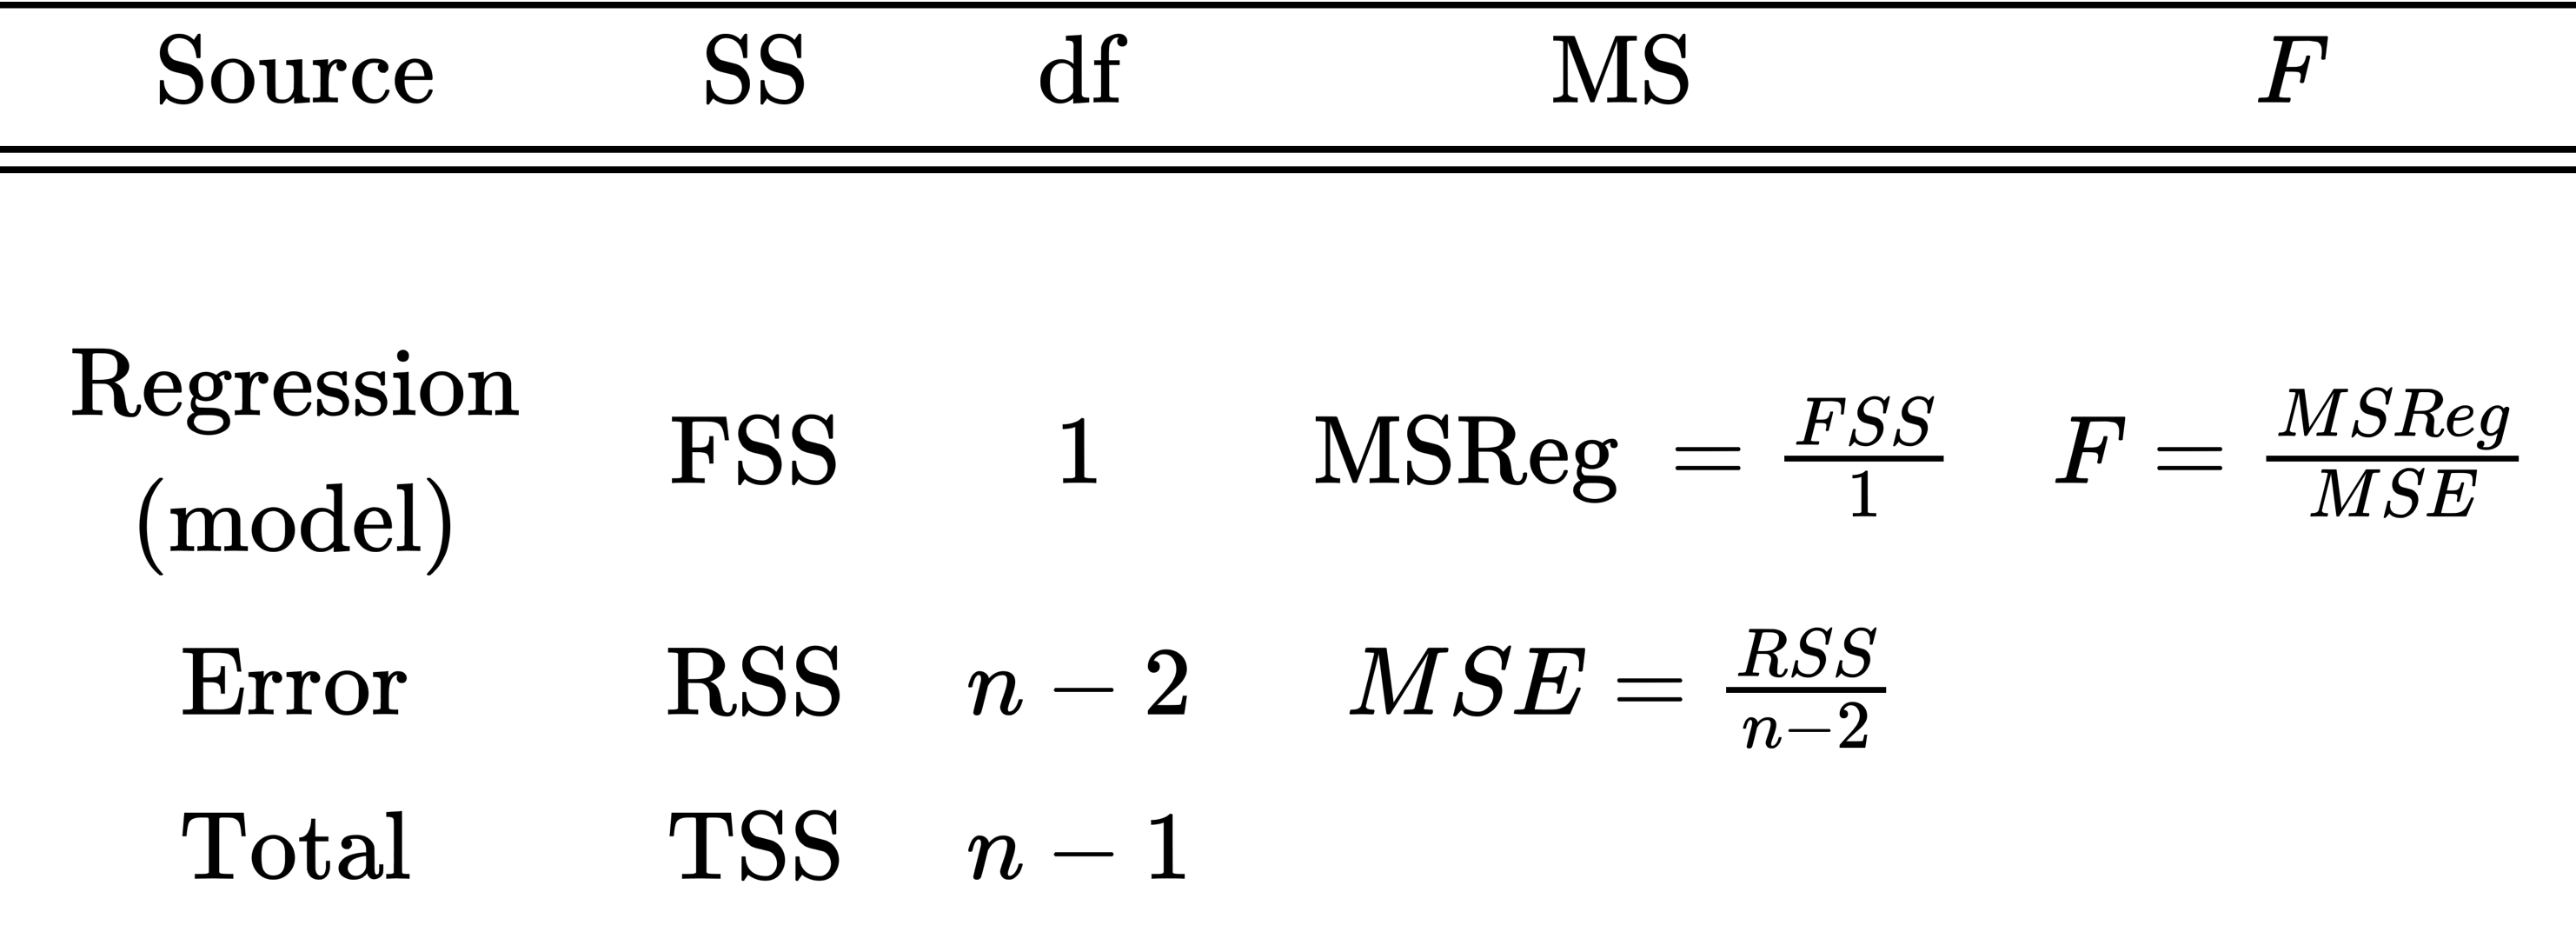
\includegraphics[scale=1]{rendered_image.png}
    \caption{}
    \label{}
\end{figure}\end{center}

\subsubsection{F-Test (equivalent to t-test)}
An alternative way to test for the model parameters is using the $F$ test:
$$
\left\{\begin{array}{l}
H_{0}: \beta_{1}=0 \\
H_{\alpha}: \beta_{1} \neq 0
\end{array}\right.
$$
- Under $H_{0}$, the $F$-test statistic is
$$
F=\frac{\text { MSReg }}{M S E}=\frac{F S S}{R S S /(n-2)} \sim F_{1, n-2}
$$
- It can be shown that the $F$-test statistic is equal to the square of the $t$-test statistic and their $p$-values are the same. So, \textbf{this test is equivalent to the $t$-test before}.

\subsection{Estimation and Prediction}

\subsubsection{Estimation (always reported for a parameter: ${\beta}_0+{\beta}_1x^*=\mathbb{E}(Y|x^*)$)}
1. Estimation: We want to estimate the mean response at $x^*$. This is equivalent to estimate: $\beta_0+\beta_1x^*$\\
2. Accuracy of the estimation: is measured by the expected value of the squared difference between the point estimate and the target.\\
- For estimation the target is $\beta_{0}+\beta_{1} x^{\star}:$
$$
\begin{aligned}
& \mathbb{E}\left(\hat{\beta}_{0}+\hat{\beta}_{1} x^{\star}-\beta_{0}-\beta_{1} x^{\star}\right)^{2} \\
=& \operatorname{Var}\left(\hat{\beta}_{0}+\hat{\beta}_{1} x^{\star}\right) \\
=& \operatorname{Var}\left(\hat{\beta}_{0}\right)+\left(x^{\star}\right)^{2} \operatorname{Var}\left(\hat{\beta}_{1}\right)+2 x^{\star} \operatorname{Cov}\left(\hat{\beta}_{0}, \hat{\beta}_{1}\right) \\
=& \sigma^{2}\left(\frac{1}{n}+\frac{\left(x^{\star}-\bar{x}\right)^{2}}{\sum_{i}\left(x_{i}-\bar{x}\right)^{2}}\right) \\
=& \sigma^{2}\left(\frac{1}{n}+\frac{\left(x^{\star}-\bar{x}\right)^{2}}{S_{x x}}\right)
\end{aligned}
$$

3. Confidence interval: An $(1-\alpha) 100 \%$ Confidence Interval for the Mean Response when $x=x^{\star}$ is given by
$$
\hat{\beta}_{0}+\hat{\beta}_{1} x^{\star} \pm T_{n-2}(\alpha / 2) \hat{\sigma} \sqrt{\frac{1}{n}+\frac{\left(x^{\star}-\bar{x}\right)^{2}}{S_{x x}}}
$$

\subsubsection{Prediction (is reported for the value of a random variable $Y^*$)}
1. Prediction: of an outcome of random variable $Y^*$ at a given value $x^*$ , where $Y^* \sim N( \beta_0 + \beta_1 x^* , \sigma^2 )$\\
2. For prediction the target is $Y^{\star}=\beta_{0}+\beta_{1} x^{\star}+e^{\star}$, where $e^{\star} \sim N\left(0, \sigma^{2}\right)$ This new error $e^{\star}$ is independent of the previous $n$ data points, i.e. is independent of $\left(\hat{\beta}_{0}, \hat{\beta}_{1}\right)$
$$
\begin{aligned}
&\mathbb{E}\left[\left(\hat{\beta}_{0}+\hat{\beta}_{1} x^{\star}-Y^{\star}\right)^{2}\right] \\
&=\mathbb{E}\left[\left(\hat{\beta}_{0}+\hat{\beta}_{1} x^{\star}-\beta_{0}-\beta_{1} x^{\star}-e^{\star}\right)^{2}\right] \\
&=\mathbb{E}\left[\left(\hat{\beta}_{0}+\hat{\beta}_{1} x^{\star}-\beta_{0}-\beta_{1} x^{\star}\right)^{2}\right]+\mathbb{E}\left[\left(e^{\star}\right)^{2}\right] \\
&=\sigma^{2}\left(1+\frac{1}{n}+\frac{\left(x^{\star}-\bar{x}\right)^{2}}{S_{x x}}\right)
\end{aligned}
$$
3. Prediction interval: An $(1-\alpha) 100 \%$ Prediction Interval for $\hat{Y}^{\star}$ when $x=x^{\star}$ is given by
$$
\hat{\beta}_{0}+\hat{\beta}_{1} x^{\star} \pm T_{n-2}(\alpha / 2) \hat{\sigma} \sqrt{1+\frac{1}{n}+\frac{\left(x^{\star}-\bar{x}\right)^{2}}{S_{x x}}}
$$
\subsubsection{Simultaneous Confidence}
$\mu^*=\mathbb{E}[y|x^*]=\beta_0+\beta_1x^*$'s Confidence Interval:
$$I(x^*)=(\hat{\mu}^*\pm T_{n-2}(\frac{\alpha}{2})se(\hat{\mu}^*))$$
Where $$\hat{\mu}^*=\hat{\beta}_0+\hat{\beta}_1x^*\text{ and }se(\hat{\mu}^*)=\hat{\sigma}\sqrt{\frac{1}{n}+\frac{(x^*-\bar{x})^2}{\sum_{i=1}^n(x_i-\bar{x})^2}}$$
If we want confidence intervals at multiple points $(x_1^*, x_2^*, \cdots, x_m^*)$, we can use formula $(1)$ to have confidence intervals at the $m$ points: $I(x_1^*), I(x_2^*), \cdots, I(x_m^*)$.\\
We know that:
$$
\mathbb{P}\left(\mu_{i}^{*} \in I\left(x_{i}^{*}\right)\right)=(1-\alpha)
$$
This is the point-wise coverage probability for $\mu_{i}^{*}$ and formula (1) gives the point-wise CI.\\
What about the simultaneous coverage probability? i.e.:
$$
\mathbb{P}\left(\mu_{i}^{*} \in I\left(x_{i}^{*}\right), \text { for } i=1, \ldots, m\right)=?
$$
To make sure that (for example):
$$
\mathbb{P}\left(\mu_{i}^{*} \in I\left(x_{i}^{*}\right), \text { for } i=1, \ldots, m\right)=.95
$$
we need to set $\alpha=5 \% / m$, which is known as the \textbf{Bonferroni correction}.\\
Let $\mathrm{A}_{k}$ denotes the event that the $k$ th confidence interval covers $\mu_{k}^{*}$ with:
$$
\mathbb{P}\left(\mathrm{A}_{k}\right)=(1-\alpha)
$$
Then we can show:
$$
\begin{aligned}
&\mathbb{P}\left(\text { All Cls cover the corresponding } \mu_{k}^{*} \text { values }\right) \\
&=\mathbb{P}\left(\mathrm{A}_{1} \cap \mathrm{A}_{2} \ldots \cap \mathrm{A}_{m}\right) \\
&=1-\mathbb{P}\left(\mathrm{A}_{1}^{c} \cup \mathrm{A}_{2}^{c} \ldots \cup \mathrm{A}_{m}^{c}\right) \\
&\geq 1-\mathbb{P}\left(\mathrm{A}_{1}^{c}\right)-\ldots-\mathbb{P}\left(\mathrm{A}_{m}^{c}\right) \\
&=1-m \alpha
\end{aligned}
$$
If we choose $\alpha / m$ instead of $\alpha$, the simultaneous coverage probability will be $(1-\alpha)$

\subsubsection{Confidence Band (Larger than CI)}
Ideally we would like to construct a simultaneous confidence band (i.e., $m=\infty$ ) across all $x^{*}$ 's. (Scheffé's Theorem - 2959 ). Let
$$
I(x)=(\hat{r}(x)-c \hat{\sigma}, \hat{r}(x)+c \hat{\sigma})
$$
where
$$
\hat{r}(x)=\hat{\beta}_{0}+\hat{\beta}_{1} x, c \hat{\sigma}=\sqrt{2 F(\alpha, 2, n-2)} \sqrt{\frac{1}{n}+\frac{(x-\bar{x})^{2}}{\sum_{i=1}^{n}\left(x_{i}-\bar{x}\right)^{2}}}
$$
Then,
$$
\mathbb{P}(r(x) \in I(x) \text { for all } x) \geq 1-\alpha
$$
Can we construct a simultaneous prediction band? No!\\
Are confidence bands always wider than point-wise confidence intervals? Yes!
For SLR, at a location $x^{*}$, we have
$$
\begin{aligned}
\text { band } &: \hat{\mu}^{*} \pm \sqrt{2 F(\alpha, 2, n-2)} \operatorname{se}\left(\hat{\mu}^{*}\right) \\
\text { interval } &: \hat{\mu}^{*} \pm T_{n-2}(\alpha / 2) \operatorname{se}\left(\hat{\mu}^{*}\right)
\end{aligned}
$$
$$
\sqrt{2 F(\alpha, 2, n-2)} > T_{n-2}(\alpha / 2)=\sqrt{2 F(\alpha, 1, n-2)}
$$
In fact, for any $\alpha$, we have
$$
T_{m}(\alpha / 2)=\sqrt{2F(\alpha, 1, m)}<\sqrt{k F(\alpha, k, m)}
$$




\subsection{Maximum likelihood estimators with normal error terms}
We start with the statistical model, which is the Gaussian-noise simple linear regression model, defined as follows:\\
1. The distribution of $X$ is arbitrary (and perhaps $X$ is even non-random).\\
2. If $X=x$, then $Y=\beta_{0}+\beta_{1} x+\epsilon$, for some constants ("coefficients", "parameters") $\beta_{0}$ and $\beta_{1}$, and some random noise variable $\epsilon$.\\
3. $\epsilon \sim N\left(0, \sigma^{2}\right)$, and is independent of $X$.\\
4. $\epsilon$ is independent across observations.\\
$$p(y_i|x_i; \beta_0,\beta_1,\sigma^2)=\frac{1}{\sqrt{2\pi\sigma^2}}e^{-\frac{1}{2}(\frac{y_i-(\beta_0+\beta_1x_i)}{\sigma})^2}$$
Given any data set $(x_1, y_1), (x_2, y_2), . . . (x_n, y_n)$, we can now write down the probability density, under the model, of seeing that data:
$$\prod_{i=1}^n p(y_i|x_i; \beta_0,\beta_1,\sigma^2)=\prod_{i=1}^n\frac{1}{\sqrt{2\pi\sigma^2}}e^{-\frac{1}{2}(\frac{y_i-(\beta_0+\beta_1x_i)}{\sigma})^2}=\frac{1}{(2\pi\sigma^2)^{\frac{n}{2}}}e^{-\frac{\sum_{i=1}^n(y_i-(\beta_0+\beta_1x_i))^2}{2\sigma^2}}$$
Take the \textbf{log-likelihood}
$$L(\beta_0,\beta_1,\sigma^2)=-\frac{n}{2}\log{2\pi}-n\log{\sigma}-\frac{1}{2\sigma^2}\sum_{i=1}^n(y_i-(\beta_0+\beta_1x_i))^2$$
Then we can compute the \textbf{Maximum likelihood estimators} $(\hat{\beta}_0,\hat{\beta}_1,\hat{\sigma}^2)$:\\
(1) $(\hat{\beta}_0,\hat{\beta}_1)$,\\
Obviously, maximizing $L(\hat{\beta}_0,\hat{\beta}_1,\hat{\sigma}^2)$ is as same as minimizing $\sum_{i=1}^n(y_i-(\hat{\beta}_0+\hat{\beta}_1x_i))^2$, then the \textbf{Maximum likelihood estimators} is exactly the \textbf{LS estimators}:
$$\begin{aligned}
    &\hat{\beta}_{1}=\frac{\sum_{i=1}^{n}\left(x_{i}-\bar{x}\right)\left(y_{i}-\bar{y}\right)}{\sum_{i=1}^{n}\left(x_{i}-\bar{x}\right)^{2}} \\
    &\hat{\beta}_{0}=\bar{y}-\hat{\beta}_{1} \bar{x}
\end{aligned}$$
(2) $\hat{\sigma}^2$,\\
And the $\hat{\sigma}^2$ is exactly the in-sample mean squared error:
$$\hat{\sigma}^2=\frac{1}{n}\sum_{i=1}^n(y_i-(\hat{\beta}_0+\hat{\beta}_1x_i))^2$$










\section{Multiple Linear Regression (MLR): Basic}
\subsection{Basic}
$x_{1}, x_{2}, \ldots, x_{p}$ be $p$ predictors of a response $y$.\\
The data will be of the form:
$\begin{array}{ccccc}y_{1} & x_{11} & x_{12} & \cdots & x_{1 p} \\ y_{2} & x_{21} & x_{22} & \cdots & x_{2 p} \\ \vdots & \vdots & \vdots & \ddots & \vdots \\ y_{n} & x_{n 1} & x_{n 2} & \cdots & x_{n p}\end{array}$

Model Equation:
$$
y_{i}=\beta_{1} x_{i 1}+\beta_{2} x_{i 2}+\cdots+\beta_{p} x_{i p}+\varepsilon_{i}, \quad i=1, \ldots, n
$$
where we denote $\mathbf{x}_{\mathbf{i}}=\left(x_{i 1, \ldots, x_{i} p}\right)^{T}$, with $x_{i 1}=1$\\
$\left(\beta_{1}, \beta_{2}, \ldots, \beta_{p} ; \sigma^{2}\right)$ are unknown true parameters.\\
$\beta_{1}$ is the intercept.\\
$\beta_{2}, \beta_{3}, \ldots, \beta_{p}$ are partial slopes.\\
$\sigma^{2}$ is the error variance
\subsubsection{Assumptions of errors}
$\varepsilon_{1}, \varepsilon_{2}, \ldots, \varepsilon_{n}$ are the random errors. They usually assumed to satisfy the same conditions as in simple linear regression:\\
- zero mean: $\mathbb{E}\left(\varepsilon_{i}\right)=0$\\
- uncorrelated: $\left.\operatorname{Cov}\left(\varepsilon_{\mathrm{i}}, \varepsilon_{\mathrm{j}}\right)=0, \mathrm{i} \neq \mathrm{j}\right)$, and\\
- homoscedastic: $\operatorname{Var}\left(\varepsilon_{\mathrm{i}}\right)=\sigma^{2}$ does not depend on $i$ ).

\subsubsection{Matrix Representation}
Matrix Representation of the MLR Model:
$$\begin{array}{cccccc}\mathbf{y}_{n \times 1} & = & \mathbf{X}_{n \times p} & \beta_{p \times 1} & + & \varepsilon_{n \times 1} \\ \uparrow & &\uparrow & \uparrow & &\uparrow \\ \text { Response }& & \text { Design } & \text { Coefficients } & &\text { Error } \\ & & \text { Matrix } & & &\text { Term }\end{array}$$
- $n:$ sample size\\
- $p:$ number of predictors or columns of $X$\\
- By default the intercept is included in the model in which case the first column of $X$ is a vector of 1 's.\\
We set $\mathbb{E}(\varepsilon)=0\text{ and }Cov(\varepsilon)=\sigma^2 \mathbf{I}_n$, then we can infer that
$$\mathbb{E}(y)= \mathbf{X}\beta,\ Cov(y)=\sigma^2 \mathbf{I}_n$$

\subsection{Parameter Estimation $\hat{\beta}=\left(\mathbf{X}^{T} \mathbf{X}\right)^{-1} \mathbf{X}^{T} y$}
- We want to estimate $\beta$, i.e. obtain:
$$
\hat{\beta}=\left(\hat{\beta}_{1}, \hat{\beta}_{2}, \ldots, \hat{\beta}_{p}\right)^{T}
$$
- The LS estimator of $\beta$ minimizes the sum of squared residuals:
$$
R S S=\|y-\mathbf{X} \beta\|^{2}=(y-\mathbf{X} \beta)^{T}(y-\mathbf{X} \beta)
$$
In order to minimize $R S S=(y-\mathbf{X} \beta)^{T}(y-\mathbf{X} \beta)$, we take derivatives with respect to $\beta$ 's and set to zero (as before).\\
$$\frac{\partial R S S}{\partial \beta}=-2 \mathbf{X}_{p \times n}^{T}(y-\mathbf{X} \beta)_{n \times 1}=\mathbf{0}_{p \times 1}$$
$\mathbf{X}^{T}(y-\mathbf{X} \beta)=\mathbf{0} \longrightarrow$ Normal Equations\\
$\left(\mathbf{X}^{T} \mathbf{X}\right) \beta=\mathbf{X}^{T} y$\\
$\hat{\beta}=\left(\mathbf{X}^{T} \mathbf{X}\right)^{-1} \mathbf{X}^{T} y \rightarrow \mathrm{LS}$ Estimators\\
\textbf{Remarks}\\
1. We assume that the rank of $X$ is $p$, i.e. no columns of $X$ is a linear combinations of the other columns of $X$.\\
2. Since $\mathbf{X}$ has rank $p$, the inverse of $\left(\mathbf{X}^{T} \mathbf{X}\right)$ exists.\\
3. if $\left(\mathbf{X}^{T} \mathbf{X}\right)$ is singular the $LS$ solutions is not unique (identifiability problem)

\subsubsection{Fitted Values $\hat{y}_{n \times 1}=\mathbf{H}_{n \times n} y_{n \times 1}$}
$$
\begin{aligned}
\hat{y}_{n \times 1} &=\mathbf{X} \hat{\beta} \\
&=\mathbf{X}\left(\mathbf{X}^{T} \mathbf{X}\right)^{-1} \mathbf{X}^{T} y \\
&=\mathbf{X}\left(\mathbf{X}^{T} \mathbf{X}\right)^{-1} \mathbf{X}^{\top} y\\&=\mathbf{H}_{n \times n} y_{n \times 1}
\end{aligned}
$$
$\mathbf{H}_{n \times n}=\mathbf{X}\left(\mathbf{X}^{T} \mathbf{X}\right)^{-1} \mathbf{X}^{\top}$ is called the hat matrix, since it returns the "y-hat" values.
\subsection{Residuals $\mathbf{r}=(\mathbf{I}-\mathbf{H}) y$, (Sample) error variance $\hat{\sigma}^2=\frac{\mathbf{r}^T \mathbf{r}}{n-p}$}
$$
\mathbf{r}_{n \times 1}=y-\hat{y}=y-\mathbf{H} y=(\mathbf{I}-\mathbf{H}) y
$$
The residuals $\mathbf{r}$ are used to estimate the error variance:
$$
\hat{\sigma}^2=\frac{1}{n-p} \sum_{i} r_{i}^{2}=\frac{\mathbf{r}^T \mathbf{r}}{n-p}=\frac{R S S}{n-p}
$$

\subsection{Properties of residuals}
The LS estimator is the $\beta$ that satisfies the normal equations, that is
$$
\mathbf{X}^{T}(y-\hat{y})=\mathbf{X}^{T}(y-\mathbf{X} \hat{\beta})=\mathbf{0}
$$
This implies the following properties for the residuals, $r_{n \times 1}=y-\mathbf{X} \hat{\beta}$ :
\subsubsection{$\mathbf{X}^{T} \boldsymbol{r}=0$}
1. The cross-products between the residual vector $r$ and each column of $\mathbf{X}$ are zero, i.e.
$$
\begin{aligned}
\mathbf{X}^{T} \boldsymbol{r} &=\mathbf{X}^{T}(\boldsymbol{y}-\mathbf{X} \hat{\boldsymbol{\beta}})=\mathbf{X}^{T} \boldsymbol{y}-\mathbf{X}^{T} \mathbf{X} \hat{\beta} \\
&=\mathbf{X}^{T} \boldsymbol{y}-\left(\mathbf{X}^{T} \mathbf{X}\right)\left(\mathbf{X}^{T} \mathbf{X}\right)^{-1} \mathbf{X}^{T} \boldsymbol{y}=0
\end{aligned}
$$
\subsubsection{$\hat{y}^{T} \boldsymbol{r}=0$}
2. The cross-product between the fitted value $\hat{y}$ and the residual vector $r$ is zero, i.e.
$$
\hat{y}^{T} r=\hat{\beta}^{T} X^{T} r=0
$$
This implies that the residual vector $r$ is \textbf{orthogonal} to each column of $X$ and $\hat{y}$.\\
\subsection{Properties of $\mathbf{H}$}
\subsubsection{$\mathbf{H X}=\mathbf{X}$}
Let $c$ be any linear combination of the columns of $\mathbb{X}$, then
$$
\mathbf{H} c=c
$$
since $\mathbf{H X}=\mathbf{X}\left(\mathbf{X}^{\top} \mathbf{X}\right)^{-1} \mathbf{X}^{T} \mathbf{X}=\mathbf{X}$
\subsubsection{Symmetric: $\mathbf{H}^{T}=\mathbf{H}$}
\textbf{Symmetric}, since $\mathbf{H}^{T}=\left(\mathbf{X}\left(\mathbf{X}^{T} \mathbf{X}\right)^{-1} \mathbf{X}^{T}\right)^{T}=\mathbf{X}\left(\mathbf{X}^{T} \mathbf{X}\right)^{-1} \mathbf{X}^{T}=\mathbf{H}$
\subsubsection{Idempotent: $\mathbf{H H}=\mathbf{H H}^{T}=\mathbf{H}^{\top} \mathbf{H}=\mathbf{H}$}
\textbf{Idempotent}, i.e. $\mathbf{H H}=\mathbf{H H}^{T}=\mathbf{H}^{\top} \mathbf{H}=\mathbf{H} .$ Indeed
$$
\mathbf{H H}=\mathbf{X}\left(\mathbf{X}^{T} \mathbf{X}\right)^{-1} \mathbf{X}^{T} \mathbf{X}\left(\mathbf{X}^{T} \mathbf{X}\right)^{-1} \mathbf{X}^{T}=\mathbf{X}\left(\mathbf{X}^{T} \mathbf{X}\right)^{-1} \mathbf{X}^{T}=\mathbf{H}
$$
\subsubsection{$\mathbf{H}(\mathbf{I}-\mathbf{H})=\mathbf{0}$}
This also implies that $\mathbf{H}(\mathbf{I}-\mathbf{H})=\mathbf{0}_{n \times n}$
\subsubsection{$(\mathbf{I}-\mathbf{H})$ is also symmetric and idempotent}
$$(\mathbf{I}-\mathbf{H})(\mathbf{I}-\mathbf{H})=(\mathbf{I}-\mathbf{H})^T(\mathbf{I}-\mathbf{H})=(\mathbf{I}-\mathbf{H})(\mathbf{I}-\mathbf{H})^T=\mathbf{I}-\mathbf{H}$$
\subsubsection{$\operatorname{trace}(\mathbf{H})=\mathrm{p}$}
$\operatorname{trace}(\mathbf{H})=\mathrm{p}$, the number of $\mathrm{LS}$ coefficients we estimated.

\subsection{Geometric Representation of LS}
\begin{center}\begin{figure}[htbp]
    \centering
    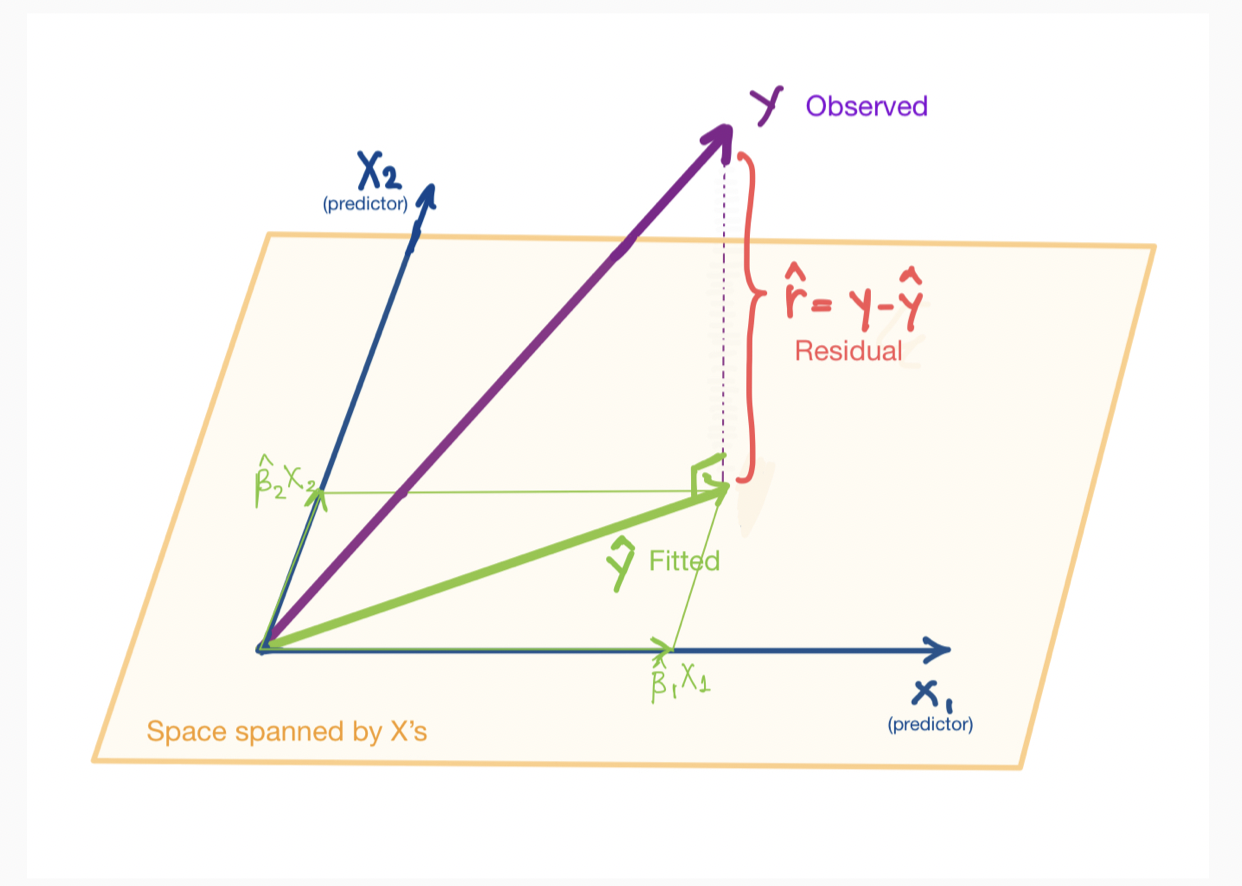
\includegraphics[scale=0.5]{截屏2021-09-05 22.22.04.png}
    \caption{}
    \label{}
\end{figure}\end{center}
\subsubsection{Estimation Space}
- The columns of $\mathbf{X}$ span a $p$-dimensional subspace in $\mathbb{R}^{n}$. This is a subspace that consists of vectors that can be written as linear combinations of the columns of $X$.\\
- The LS squares estimator $\hat{\beta}$ is obtained by minimizing the Euclidean distance between the vectors $\mathbf{y}$ and $\hat{\mathbf{y}}$, i.e. $\|y-\hat{y}\|^{2}$. $\hat{y}$ is the projection of $y$ onto the estimation space.\\
- $\mathbf{H}_{n \times n}$, projection/hat matrix is symmetric, unique, and idempotent.\\
\subsubsection{Error Space}
- The error space is an $(n-p)$-dimensional space that is orthogonal to the estimation space. The projection matrix of the error space is $(\mathbf{I}-\mathbf{H})$.\\
- The residual $\mathbf{r}$ is the projection of $\boldsymbol{y}$ onto the error space, orthogonal to the estimation space. So, $\mathbf{r}$ is orthogonal to any vector in the estimation space, including each column of $X$.\\
- When the intercept is included in the model, then
$$
\sum_{i=1}^{n} r_{i}=0
$$
In general, $\sum_{i=1}^{n} r_{i} X_{i j}=0, j=1, \ldots, p$ due to the normal equations.

\subsection{Coefficient of determination, $R-$Square}
$$
R^{2}=1-\frac{\sum_{i}\left(\hat{y}_{i}-y_{i}\right)^{2}}{\sum_{i}\left(y_{i}-\bar{y}\right)^{2}}=1-\frac{R S S}{T S S}
$$
An equivalent definition is
$$
R^{2}=\frac{\sum_{i}\left(\hat{y}_{i}-\bar{y}\right)^{2}}{\sum_{i}\left(y_{i}-\bar{y}\right)^{2}}
$$
$0 \leq R^{2} \leq 1$
\subsection{Properties of LS Estimators}
\subsubsection{Unbiased: $\mathbb{E}(\hat{\beta})=\beta$}
\begin{equation}
    \begin{aligned}
        \mathbb{E}(\hat{\beta})&=\mathbb{E}(\left(\mathbf{X}^{T} \mathbf{X}\right)^{-1} \mathbf{X}^{T} y)=\left(\mathbf{X}^{T} \mathbf{X}\right)^{-1} \mathbf{X}^{T} \mathbb{E}(y)\\
        &=\left(\mathbf{X}^{T} \mathbf{X}\right)^{-1} \mathbf{X}^{T}\mathbf{X}\beta=\beta
    \end{aligned}
    \nonumber
\end{equation}

\subsubsection{Variance-Covariance Matrix of $\hat{\beta}$: $\operatorname{Cov}(\hat{\beta})=\sigma^{2}\left(\mathbf{X}^{T} \mathbf{X}\right)^{-1}$}
$$\begin{aligned} \operatorname{Cov}(\hat{\beta}) &=\left(\mathbf{X}^{T} \mathbf{X}\right)^{-1} \mathbf{X}^{T} \operatorname{Cov}(\mathbf{y})\left(\left(\mathbf{X}^{\top} \mathbf{X}\right)^{-1} \mathbf{X}^{\top}\right)^{\top} \\ &=\left(\mathbf{X}^{T} \mathbf{X}\right)^{-1} \mathbf{X}^{T} \sigma^{2} \mathbf{X}\left(\mathbf{X}^{\top} \mathbf{X}\right)^{-1} \\ &=\sigma^{2}\left(\mathbf{X}^{T} \mathbf{X}\right)^{-1} \mathbf{X}^{\top} \mathbf{X}\left(\mathbf{X}^{T} \mathbf{X}\right)^{-1} \\ &=\sigma^{2}\left(\mathbf{X}^{T} \mathbf{X}\right)^{-1} \end{aligned}$$
$$se(\hat{\beta}_i)=\hat{\sigma}\sqrt{((\mathbf{X}^T\mathbf{X})^{-1})_{ii}}$$


\subsubsection{$\hat{y}$: $\mathbb{E}(\hat{y})=\mathbf{X}\beta$, $Cov(\hat{y})=\sigma^2 \mathbf{H}$}
\begin{equation}
    \begin{aligned}
        &\mathbb{E}(\hat{y})=\mathbb{E}(\mathbf{X}\left(\mathbf{X}^{T} \mathbf{X}\right)^{-1} \mathbf{X}^{\top}y)=\mathbf{X}\left(\mathbf{X}^{T} \mathbf{X}\right)^{-1} \mathbf{X}^{\top}\mathbf{X}\beta=\mathbf{X}\beta\\
        &Cov(\hat{y})=Cov(\mathbf{H}y)=\mathbf{H}Cov(y)\mathbf{H}^T=\sigma^2\mathbf{H}\mathbf{H}^T=\sigma^2\mathbf{H}
    \end{aligned}
    \nonumber
\end{equation}
\subsubsection{$\mathbf{r}$: $\mathbb{E}(\mathbf{r})=0$, $Cov(\mathbf{r})=\sigma^2 (\mathbf{I}_n-\mathbf{H})$}
\begin{equation}
    \begin{aligned}
        &\mathbb{E}(\mathbf{r})=\mathbb{E}(y-\hat{y})=0\\
        &Cov(\mathbf{r})=Cov(y-\hat{y})=Cov((\mathbf{I}-\mathbf{H})y)=\sigma^2(\mathbf{I}-\mathbf{H})(\mathbf{I}-\mathbf{H})^T=\sigma^2(\mathbf{I}-\mathbf{H})
    \end{aligned}
    \nonumber
\end{equation}
\subsubsection{$\mathbb{E}(\hat{\sigma}^2)=\sigma^2$}
$$\mathbb{E}(\hat{\sigma}^2)=\frac{1}{n-p}\mathbb{E}(\mathbf{r}^T \mathbf{r})=\frac{1}{n-p}\sigma^2(n-p)=\sigma^2$$
$n-p$来自于: 有$p$个元素在H对角中为$1$,其余为$0$,所以$\mathbf{I}_n-\mathbf{H}$对角中有$n-p$个1。所以只有$n-p$个$r_i^2=\sigma^2$
$$\frac{\mathbf{r}^T \mathbf{r}}{\sigma^2}=\frac{RSS}{\sigma^2}\sim \chi^2_{n-p}$$

\subsection{The Gauss-Markov Theorem: LS estimator is the \textbf{BLUE}(best linear unbiased estimator)}
If the errors are 1. Mean zero, 2. umcorrelated, 3. homoscedastic, the LS estimators have \textbf{the lowest variance within the class of linear estimators.}\\
Suppose we are interested in estimating a linear combination of $\beta$ of the form:
$$\theta=\mathbf{c}^T\beta=\sum_{j=1}^pc_j\beta_j$$
LS estimators:
$$\hat{\theta}_{LS}=\mathbf{c}^T\hat{\beta}=\mathbf{c}^T \left(\mathbf{X}^{T} \mathbf{X}\right)^{-1} \mathbf{X}^{T} y$$
This is a \textbf{linear} (linear combination of $y_1,y_2,...,y_n$) and \textbf{unbiased estimator} of $\theta$. Its mean square error can be calculated as:
$$
MSE( \hat{\theta}_{LS} ) = \mathbb{E}( \hat{\theta}_{LS} − \theta)^2 = Var( \hat{\theta}_{LS})$$
\begin{theorem}[Gauss-Markov Theorem]
    $\hat{\theta}_{LS}=\mathbf{c}^T\hat{\beta}$ is the \textbf{BLUE}(best linear unbiased estimator) of the parameter $\mathbf{c}^T\beta$ for any vector $\mathbf{c}\in \mathbb{R}^p$
\end{theorem}

\subsection{Maximum Likelihood Estimation, Distribution of LS estimates}
\subsubsection{$\mathbf{y} \sim \mathbf{N}_{n}\left(\mathbf{X} \beta, \sigma^{2} \mathbf{I}\right)$}
Recall the normality assumption for the regression model:
$$
y_{i}=\mathbf{x}_{i}^{T} \beta+\varepsilon_{i},\quad i=1, \ldots, n, \text { with } \varepsilon_{i} \sim N\left(0, \sigma^{2}\right)
$$
This implies that $\mathbf{y} \sim \mathbf{N}_{n}\left(\mathbf{X} \beta, \sigma^{2} \mathbf{I}\right)$

\subsubsection{LS estimator is the Maximum Likelihood Estimator (MLE)}
We can show that the likelihood function can be written as:
$$
L\left(\beta, \sigma^{2} \mid \mathbf{y}\right) \propto \frac{R S S}{n}^{-\frac{n}{2}}
$$
The value of $\beta$ that maximizes the Likelihood function is \textit{the Maximum Likelihood Estimator (MLE)} of $\beta$. This estimator is equal to the LS estimate of $\beta$.
\subsubsection{$\hat{\beta}\sim \mathbf{N}_{\mathbf{p}}\left(\beta, \sigma^{2}\left(\mathbf{X}^{\top} \mathbf{X}\right)^{-1}\right)$, $\hat{\mathbf{y}}\sim\mathbf{N}_{\mathbf{n}}\left(\mathbf{X} \beta, \sigma^{2} \mathbf{H}\right)$, $\hat{\mathbf{r}}\sim \mathbf{N}_{\mathbf{n}}\left(\mathbf{0}, \sigma^{2}\left(\mathbf{I}_{\mathbf{n}}-\mathbf{H}\right)\right)$}
Recall the assumption for the linear regression model:
$$
\mathbf{y} \sim \mathbf{N}_{\mathbf{n}}\left(\mathbf{X} \beta, \sigma^{2} \mathbf{I}\right)
$$
Any affine transformation of $\mathbf{y}$ will also have a Normal distribution $^{2}$.
We can show that:
$$
\begin{gathered}
\hat{\beta}=\left(\mathbf{X}^{\top} \mathbf{X}\right)^{-1} \mathbf{X}^{\top} \mathbf{y} \sim \mathbf{N}_{\mathbf{p}}\left(\beta, \sigma^{2}\left(\mathbf{X}^{\top} \mathbf{X}\right)^{-1}\right) \\
\hat{\mathbf{y}}=\mathbf{H} \mathbf{y} \sim \mathbf{N}_{\mathbf{n}}\left(\mathbf{X} \beta, \sigma^{2} \mathbf{H}\right) \\
\hat{\mathbf{r}}=\left(\mathbf{I}_{\mathbf{n}}-\mathbf{H}\right) \mathbf{y} \sim \mathbf{N}_{\mathbf{n}}\left(\mathbf{0}, \sigma^{2}\left(\mathbf{I}_{\mathbf{n}}-\mathbf{H}\right)\right)
\end{gathered}
$$
\subsection{$\mathbf{r}$ Residuals’ Properties}
\subsubsection{$\mathbf{r}\in \mathbb{R}^{n-p}$}
Although $\mathbf{r}$ is a vector of dimension $n$, it always lies in a subspace of dimension $(n − p)$.
\subsubsection{$\hat{\sigma}^{2}\sim\sigma^{2} \frac{\chi_{n-p}^{2}}{n-p}$}
r behaves like a random vector with a distribution $\mathbf{N}_{n-p}\left(\mathbf{0}, \sigma^{2} \mathbf{I}_{n-p}\right)$, so we have:
$$
\hat{\sigma}^{2}=\frac{\|\mathbf{r}\|^{2}}{n-p} \sim \sigma^{2} \frac{\chi_{n-p}^{2}}{n-p}
$$
\subsubsection{$\hat{\mathbf{y}}$ and $\boldsymbol{r}$ are independent}
It can be show that $\hat{\mathbf{y}}$ and $\boldsymbol{r}$ are uncorrelated since they are in orthogonal spaces. Since they also have a joint normal distribution, they are independent.

\subsection{Testing Predictors (Coefficients)}
\subsubsection{Testing a Single Predictor $H_0: \beta_j=0$: $t-$test}
Suppose you have a $p$ predictors in your regression model and you want to test the hypothesis:
$$
H_{0}: \beta_{j}=c \text { vs. } H_{\alpha}: \beta_{j} \neq c
$$
- The t-test statistic we use is:
$$
t=\frac{\hat{\beta}_{j}-c}{s e\left(\hat{\beta}_{j}\right)}=\frac{\hat{\beta}_{j}-c}{\hat{\sigma} \sqrt{\left[\left(\mathbf{X}^{\top} \mathbf{X}\right)^{-1}\right]_{j j}}} \sim T_{n-p}
$$
under the null hypothesis $H_{0}$.\\
- p-value $=2 \times$ the area under the curve of a $T_{n-p}$ distribution more extreme than the observed statistic.\\
- The $p$-value returned by the $I m$ function command is for $c=0$.
\subsubsection{Review the degree of freedom}
The degrees of freedom of a $t$-test are determined by the \underline{denominator} of the estimated variance $\hat{\sigma}^{2}$. Consider the following situations:\\
- In STAT 400: Test for $\theta=\alpha$, where $Z_{1}, \ldots, Z_{n} \sim \mathcal{N}\left(\theta, \sigma^{2}\right)$
$$
\frac{\hat{\theta}-\alpha}{\operatorname{se}(\hat{\theta})}=\frac{\overline{\mathbf{Z}}-\alpha}{\sqrt{\hat{\sigma}^{2} / n}} \sim T_{n-1}, \quad \hat{\sigma}^{2}=\frac{\sum_{i}\left(Z_{i}-\bar{Z}\right)^{2}}{n-1}
$$
- In SLR: Test for $\beta_{1}=c$, we have
$$
\frac{\hat{\beta}_{1}-c}{\operatorname{se}\left(\hat{\beta}_{1}\right)}=\frac{\hat{\beta}_{1}-c}{\hat{\sigma} / \sqrt{S_{X X}}} \sim T_{n-2},\quad \hat{\sigma}^{2}=\frac{R S S}{n-2}
$$
- In $M L R$ with $p$ predictors (including the intercept): Test for $\beta_{j}=c$,
$$
\frac{\hat{\beta}_{j}-c}{\operatorname{se}\left(\hat{\beta}_{j}\right)}=\frac{\hat{\beta}_{j}-c}{\hat{\sigma} \sqrt{\left[\left(\mathbf{X}^{T} \mathbf{X}\right)^{-1}\right]_{j j}}} \sim T_{n-p}, \quad\hat{\sigma}^{2}=\frac{R S S}{n-p}
$$

\subsubsection{Testing all predictors: $F-$test}
Testing all predictors
$$
\left\{\begin{array}{l}
H_{0}: \beta_{2}=\beta_{3}=\ldots=\beta_{p}=0 \\
H_{a}: \beta_{j} \neq 0, \quad \text { for some } j, j=2, \ldots, p
\end{array}\right.
$$
- Under the Null hypothesis, the test statistic:
$$
\begin{aligned}
F &=\frac{F S S\left(X_{2}, \ldots, X_{p}\right)}{p-1} \div \frac{R S S\left(X_{2}, \ldots, X_{p}\right)}{n-p} \\
&=\frac{M S(R e g)}{M S(\text { Error })} \sim F_{p-1, n-p}
\end{aligned}
$$
Large values of $F$ lead to conclusion $H_{\alpha}$.\\
- This is the overall $F$ test of whether or not there is a regression relation between the response variable $Y$ and the set of $X$ variables.
\begin{center}\begin{figure}[htbp]
    \centering
    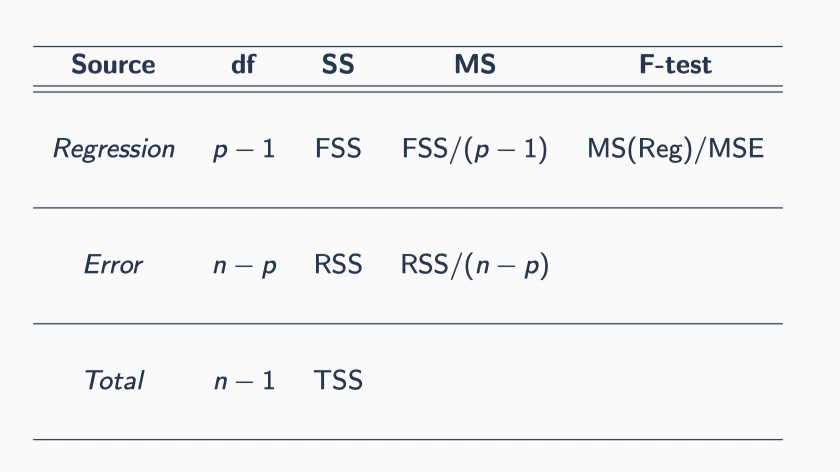
\includegraphics[scale=0.8]{Lec0601.png}
    \caption{}
    \label{}
\end{figure}\end{center}
\subsubsection{Partial $F-$test}
In general, consider the following partition of the design matrix into two sub-matrices $\mathbf{X}_{1}$ and $\mathbf{X}_{2}$, that is
$$
\mathbf{X}_{n \times p}=\left(\mathbf{X}_{1 n \times(p-q)}, \mathbf{X}_{2 n \times q}\right)
$$
The corresponding partition of the regression parameter is:
$$
\beta^{T}=\left(\beta_{1}^{T}, \beta_{2}^{T}\right)
$$
where $\beta_{1}$ is $(p-q) \times 1$ and $\beta_{2}$ is $q \times 1$\\
This partition is used to test the hypothesis:
$$
\left\{\begin{array}{l}
H_{0}: \beta_{2}=\mathbf{0}, \text { i.e., } \quad \mathbf{y}=\mathbf{X}_{1} \beta_{1}+\text { error } \\
H_{\alpha}: \beta_{2} \neq \mathbf{0}, \text { i.e., }\quad \mathbf{y}=\mathbf{X}_{1} \beta_{1}+\mathbf{X}_{2} \beta_{2}+\text { error }
\end{array}\right.
$$
To test this hypothesis, the test statistic is:
$$
F=\frac{\left(R S S_{0}-R S S_{\alpha}\right) / q}{R S S_{\alpha} /(n-p)} \sim F_{q, n-p}
$$
where \textbf{$R R S_{0}=$ Residual sum of squares for the model under $H_{0}$ ; $R R S_{a}=$ Residual sum of squares for the model under $H_{\alpha}$}

\textbf{Numerator}: variation in the data not explained by the reduced model, but explained by the full model.

\textbf{Denominator}: variation in the data not explained by the full model (i.e., not explained by either model), which is used to estimate the error variance.

\textit{Reject $H_{0}$, if $F$ test statistic is large}, that is, the variation missed by the reduced model, when being compared with the error variance, is significantly large.

F-test statistic can be rewirtten:
$$F=\frac{(RSS_{0}-RSS_{\alpha})/q}{RSS_{\alpha}/(n-p)}=\frac{((1-R_R^2)-(1-R_F^2))/(df_F-df_R)}{(1-R_F^2)/df_F}=\frac{(R_F^2-R_R^2)/(df_R-df_F)}{(1-R_F^2)/df_F}$$
Note that this test statistic is not appropriate when the full and reduced regression models do not contain the intercept term $\beta_0$ .

\subsection{Permutation Tests (When the normal distribution hypothesis doesn't hold)}
The distribution of the data is \textit{unknown}.
- A test statistic is a function of the data; denote it $g($ data $)$.\\
- The test statistic tends to take extreme values under the alternative hypothesis $H_{\alpha}$.
\subsubsection{Procedure}
Procedure to conduct a permutation test\\
1. Form the test statistic $g($ data $)$ which tends to take extreme values under the alternative hypothesis.\\
2. Evaluate the test statistic on the observed data, denoted by $g_{0}$.\\
3. Find the distribution of $g($ data $)$, when data are generated from $H_{0}$.\\
4. Calculate the $p$-value, that is the following probability:
\begin{center}
    $\mathbb{P}\left(g(\right.$ data $)$ is more extreme than the observed $g_{0} \mid$ data $\left.\sim H_{0}\right)$
\end{center}

\subsubsection{Calculation of the p-value: Monte Carlo method}
We can obtain an approximation of $\mathbb{E}(Y)$ as follows:\\
1. Generate $N=1000$ samples from this distribution, $Y_{1}, \ldots, Y_{N}$\\
2. Approximate the mean by
$$
\mathbb{E}(Y) \approx \frac{1}{N} \sum_{i=1}^{N} Y_{i}
$$
That is, population mean $\approx$ sample mean (when $N$ is large).\\

This method also works if we want to approximate the expected value of a \textit{function} of a random variable:
$$
\mathbb{E}(f(Y)) \approx \frac{1}{N} \sum_{i=1}^{N} f\left(Y_{i}\right)
$$

\subsection{Confidence Intervals for $\beta_j$, Confidence Region for $\beta$}
\subsubsection{Confidence Intervals for $\beta_j$}
Recall that
$$\hat{\beta}=\left(\mathbf{X}^{\top} \mathbf{X}\right)^{-1} \mathbf{X}^{\top} \mathbf{y} \sim \mathbf{N}_{\mathbf{p}}\left(\beta, \sigma^{2}\left(\mathbf{X}^{\top} \mathbf{X}\right)^{-1}\right)$$
An $(1-\alpha)100\%$ CI(Confidence Interval) for $\beta_j$ can be written as
$$(\hat{\beta}_j \pm T_{n-p}(\frac{\alpha}{2})se(\hat{\beta}_j))=(\hat{\beta}_j \pm T_{n-p}(\frac{\alpha}{2})\hat{\sigma}\sqrt{[\left(\mathbf{X}^{\top} \mathbf{X}\right)^{-1}]_{jj}})$$
Justification: The vector $\beta$'s confidence interval is a family/joint interval for all the betas, so it will be
wider than the individual $\beta_j$’s intervals.
\subsubsection{Confidence Region for $\beta$}
$\beta$ is the entire vector,
$$\beta-\hat{\beta}\sim\mathbf{N}_{\mathbf{p}}\left(0, \sigma^{2}\left(\mathbf{X}^{\top} \mathbf{X}\right)^{-1}\right)$$
Thus the quadratic form:
$$\frac{(\beta-\hat{\beta})^T \mathbf{X}^T \mathbf{X}(\beta-\hat{\beta})}{p \hat{\sigma}^2}\sim F_{p,n-p}$$
We can construct a $(1-\alpha)100\%$ confidence region for $\beta$ to be all the points in the following ellipsoid,
$$\frac{(\beta-\hat{\beta})^T \mathbf{X}^T \mathbf{X}(\beta-\hat{\beta})}{p \hat{\sigma}^2}<F(\alpha; p,n-p)$$
Where $F(\alpha; p,n-p)$ is defined to be the point such that $$\mathbb{P}(F_{p,n-p}>F(\alpha; p,n-p))=\alpha$$
\begin{center}\begin{figure}[htbp]
    \centering
    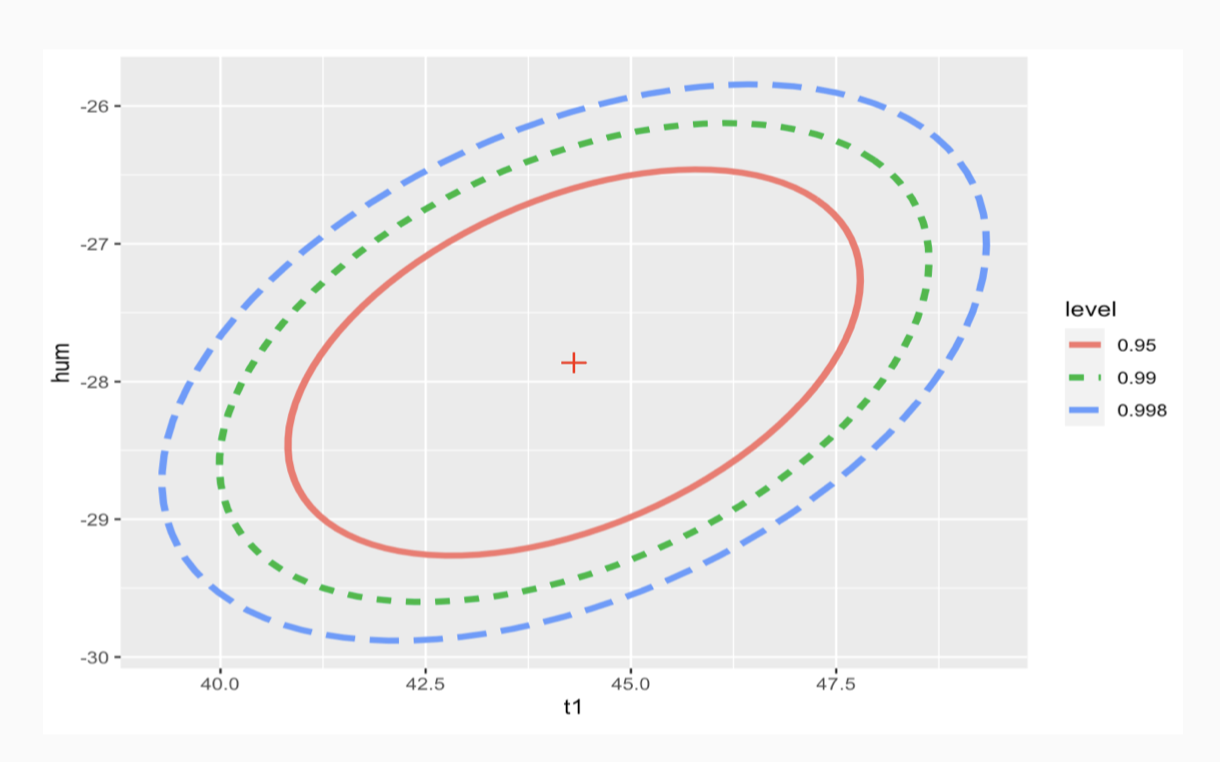
\includegraphics[scale=0.5]{Lec0701.png}
    \caption{}
    \label{}
\end{figure}\end{center}

\subsection{Confidence/Prediction Intervals for New Observations}
Set $\mathbb{E}(Y|x^*)=\mu^*=(x^*)^T\beta$
\subsubsection{Confidence Interval for $\mu^*=(x^*)^T\beta$}
The Gauss-Markov theorem tells us that the BLUE (Best Linear Unbiased Estimate) of $\mu^*$ is:
$$\hat{\mu}^*=(x^*)^T \hat{\beta}=(x^*)^T(X^TX)^{-1}X^Ty$$
Then,
\begin{equation}
    \begin{aligned}
        \mathbb{E}[(\hat{\mu}^*-\mu^*)^2]&=Var(\hat{\mu}^*)\\
        &=\sigma^2(x^*)^T(X^TX)^{-1}x^*\\
        se(\hat{\mu}^*)&=\hat{\sigma}\sqrt{(x^*)^T(X^TX)^{-1}x^*}
    \end{aligned}
    \nonumber
\end{equation}
Where $$\frac{\hat{\mu}^*-\mu}{se(\hat{\mu}^*)} \sim t(n-p)$$
A $(1-\alpha)100\%$ CI (confidence interval) for $\mu^*$ is:
$$\hat{\mu}^*\pm T_{n-p}(\frac{\alpha}{2})se(\hat{\mu}^*)$$
\subsubsection{Prediction Interval for $y^*=(x^*)^T\beta+e^*$}
The best estimate for $y^*$ at a future observation $x^*$ is also
$$\hat{y}^*=(x^*)^T \hat{\beta}$$
Then,
\begin{equation}
    \begin{aligned}
        Var(\hat{y}^*)&=\mathbb{E}[((x^*)^T \hat{\beta}-y^*)^2]\\
        &=\mathbb{E}[((x^*)^T \hat{\beta}-((x^*)^T\beta+e^*))^2]\\
        &=\mathbb{E}[((x^*)^T \hat{\beta}-((x^*)^T\beta)^2]+\mathbb{E}[(e^*)^2]\\
        &=Var(\hat{\mu}^*)+Var(e)\\
        &=\sigma^2[1+(x^*)^T(X^TX)^{-1}x^*]\\
        se(\hat{y}^*)&=\hat{\sigma}\sqrt{1+(x^*)^T(X^TX)^{-1}x^*}
    \end{aligned}
    \nonumber
\end{equation}
Where $$\frac{\hat{y}^*-y^*}{se(\hat{y}^*)} \sim t(n-p)$$
A $(1-\alpha)100\%$ PI (prediction interval) for $y^*$ is:
$$\hat{y}^*\pm T_{n-p}(\frac{\alpha}{2})se(\hat{y}^*)$$

\subsubsection{Mahalanobis distance}
$$\mathbf{X}_{n\times p}=\begin{bmatrix}
    \mathbf{x}_1&\mathbf{x}_2&\cdots&\mathbf{x}_n
\end{bmatrix}^T$$
For any observation vector $\mathbf{x}_{p\times 1}=\begin{pmatrix}
    1\\
    \mathbf{z}
\end{pmatrix}$, where $\mathbf{z}$ denotes the value of predictors without the intercept.\\
We would like to use \textbf{Mahalanobis distance} to quantify the distance between observation vector $\mathbf{x}_{p\times 1}$ and its sample meaning $\bar{\mathbf{x}}$.\\
The sample convariance matrix of $\mathbf{Z}=\begin{bmatrix}
    \mathbf{z}_1&\mathbf{z}_2&\cdots&\mathbf{z}_n\\
\end{bmatrix}$ is:
$$\hat{\Sigma}_{(p-1)\times(p-1)}=\frac{1}{n-1}\sum_{i=1}^n(\mathbf{z}_i-\bar{\mathbf{z}})(\mathbf{z}_i-\bar{\mathbf{z}})^T$$
Then the $(x^*)^T(X^TX)^{-1}x^*$ can be written as
\begin{equation}
    \begin{aligned}
        (x^*)^T(X^TX)^{-1}x^*=\frac{1}{n}+\underline{\frac{1}{n-1}(\mathbf{z}^*-\bar{\mathbf{z}})^T\hat{\Sigma}^{-1}(\mathbf{z}^*-\bar{\mathbf{z}})}
    \end{aligned}
    \nonumber
\end{equation}
The second term in the right hand side ($\frac{1}{n-1}(\mathbf{z}^*-\bar{\mathbf{z}})^T\hat{\Sigma}^{-1}(\mathbf{z}^*-\bar{\mathbf{z}})$) is the so-called Mahalanobis distance from $\mathbf{z}^*$ to the center of the data $\bar{\mathbf{z}}$ (the sample mean).\\
Then we can write,
$$
\begin{aligned}
\operatorname{se}\left(\hat{\mu}^{*}\right) &=\hat{\sigma} \sqrt{\mathbf{x}^{* \top}\left(\mathbf{X}^{\top} \mathbf{X}\right)^{-1} \mathbf{x}^{*}} \\
&=\hat{\sigma} \sqrt{\frac{1}{n}+\frac{1}{n-1}\left(\mathbf{z}^{*}-\overline{\mathbf{z}}\right)^{T} \hat{\Sigma}^{-1}\left(\mathbf{z}^{*}-\overline{\mathbf{z}}\right)} \\
se\left(\hat{y}^{*}\right) &=\hat{\sigma} \sqrt{1+\left(\mathbf{x}^{*}\right)^{\top}\left(\mathbf{X}^{\top} \mathbf{X}\right)^{-1} \mathbf{x}^{*}} \\
&=\hat{\sigma} \sqrt{1+\frac{1}{n}+\frac{1}{n-1}\left(\mathbf{z}^{*}-\overline{\mathbf{z}}\right)^{T} \hat{\Sigma}^{-1}\left(\mathbf{z}^{*}-\overline{\mathbf{z}}\right)}
\end{aligned}
$$
Since $\operatorname{se}\left(\hat{y}^{*}\right)$ has an extra 1, when the sample size $n$ goes to infinity,
$$
\begin{aligned}
&\operatorname{se}\left(\hat{\mu}^{*}\right) \rightarrow 0 \\
&\operatorname{se}\left(\hat{y}^{*}\right) \rightarrow \sigma
\end{aligned}
$$

\section{MLR: unusual observations}
Recall, that we can write the MLR model as:
$$
\mathbf{y} \sim \mathcal{N}\left(\mathbf{X} \beta, \sigma^{2} \mathbf{I}_{n}\right)
$$
$-$ Error: assumed to be iid, $\varepsilon_{i} \sim \mathcal{N}\left(0, \sigma^{2}\right)$\\
$-$ Model: assumed to be linear in the parameters, i.e., $\mathbb{E}(\mathbf{y})=\mathbf{X} \beta$\\
We might have unusual observations.




\subsection{$1.$ High leverage points: $h_i\geq \frac{2p}{n}$}
\subsubsection{Leverage Points}
The diagonal elements of $\mathbf{H}=\mathbf{X}\left(\mathbf{X}^{T} \mathbf{X}\right)^{-1} \mathbf{X}^{\top}$,
$$
h_{i}=H_{i i}=\mathbf{x}_i\left(\mathbf{X}^{T} \mathbf{X}\right)^{-1} \mathbf{x}_i^{\top}=\frac{Var(x_i^T \hat{\beta})}{\sigma^2}
$$
are called \textbf{leverages} and are very useful diagnostics.
$h_{i}$ gives a measure (invariant under any affine transformation of $\mathbf{X}$ ) of how far the $i$-th observation is from the center of the data (in the $X$-space).\\
For simple linear regression:
$$
h_{i}=\frac{1}{n}+\frac{\left(x_{i}-\bar{x}\right)^{2}}{\sum_{i}\left(x_{i}-\bar{x}\right)^{2}}
$$
In general:
$$
\begin{aligned}
h_{i} &=\mathbf{x}_{\mathbf{i}}^{\boldsymbol{T}}\left(\mathbf{X}^{\top} \mathbf{X}\right)^{-1} \mathbf{x}_{\mathbf{i}} \\
&=\frac{1}{n}+\frac{1}{n-1}\left(\mathbf{z}_{i}-\overline{\mathbf{z}}\right)^{T} \hat{\boldsymbol{\Sigma}}^{-1}\left(\mathbf{z}_{i}-\overline{\mathbf{z}}\right)
\end{aligned}
$$
where
$$
\hat{\Sigma}_{(p-1) \times(p-1)}^{-1}=\frac{1}{n-1} \sum_{i=1}^{n}(\mathbf{z}-\overline{\mathbf{z}})(\mathbf{z}-\overline{\mathbf{z}})^{T}
$$
is the sample covariance of the $(p-1)$ predictor variables. The second term in the right hand side ($\frac{1}{n-1}\left(\mathbf{z}_{i}-\overline{\mathbf{z}}\right)^{T} \hat{\boldsymbol{\Sigma}}^{-1}\left(\mathbf{z}_{i}-\overline{\mathbf{z}}\right)$) is the so-called \textbf{Mahalanobis distance} from $\mathbf{z}_{i}$ to the data center $\overline{\mathbf{z}}$
\subsubsection{Properties of the Leverage: $0<h_{i}<1, \quad \sum_{i} h_{i}=p$}
Recall that the hat matrix is idempotent $\mathbf{H}=\mathbf{H H}^{\top}$ and has $\operatorname{tr}(\mathbf{H})=p$\\
These imply that
$$
\sum_{i} h_{i}=p \text { and } \sum_{j} H_{i j}^{2}=h_{i}
$$
For a given $i$ we can decompose the last sum as follows:
$$
\begin{gathered}
\sum_{j} H_{i j}^{2}=H_{i i}^{2}+\sum_{i \neq j} H_{i j}^{2}=h_{i} \\
\Rightarrow \sum_{i \neq j} H_{i j}^{2}=h_{i}\left(1-h_{i}\right) \Rightarrow h_{i}\left(1-h_{i}\right)>0
\end{gathered}
$$
From this we can conclude the following properties of $h_{i}$ :
$$
0<h_{i}<1, \quad \sum_{i} h_{i}=p
$$

\subsubsection{Fitted Values and Leverage: $Var(\hat{y}_i)=\sigma^2 h_i,\ Var(r_i)=\sigma^2(1-h_i)$}
Recall the equation $\hat{\mathbf{y}}=\mathbf{H}\mathbf{y}$.\\
\begin{equation}
    \begin{aligned}
        \hat{y}_i&=\sum_{t=1}^nH_{it}y_t\\
        &=h_iy_i+\sum_{t\neq i}^nH_{it}y_t
    \end{aligned}
    \nonumber
\end{equation}
This means that $h_i=\frac{d \hat{y}_i}{d y_i}$\\
When $h_i$ is \textbf{large (close to 1)}, $\hat{y}_i$ relies heavily on $y_i$ (instead of using the information from other data points), therefore $\hat{y}_i$ will be “forced” to be \textbf{close} to the observed $y_i$.\\
Consequently, the variance for the residual $r_i$ will be small, and the variance for the fit $\hat{y}_i$ will be large (since the fit from another data set would be quite different).
$$Var(\hat{y}_i)=\sigma^2 h_i,\ Var(r_i)=\sigma^2(1-h_i)$$

\subsubsection{High-leverage Points: $h_i\geq \frac{2p}{n}$}
\textit{Good high-leverage points}: its $y$ point follows the pattern of the rest of the data, but with an $x_i$ value that is far away from the sample mean.\\
\textit{Bad high-leverage points}: its $y$ value does not follow the pattern suggested by the rest of the data; the LS fitting might change a lot if we remove this point.\\

\subsection{Residuals: Standardized Residuals vs. Studentized residuals}
The residuals $r_i=y_i-\hat{y}_i$ do not have a constant variance. So they need to be standardized.
\subsubsection{Difference between $\varepsilon$ and $\mathbf{r}$}
$\varepsilon$ : true residuals (our theoretical quantities)\\
$\mathbf{r}$ : estimated residuals
- Both residuals are normally distributed, but:
$$
\varepsilon \sim \mathcal{N}_{n}\left(\mathbf{0}, \sigma^{2} \mathbf{I}_{n}\right), \quad \mathbf{r} \sim \mathcal{N}_{n}\left(\mathbf{0}, \sigma^{2}\left(\mathbf{I}_{n}-\mathbf{H}\right)\right)
$$
where $\mathbf{H}$ is the projection/hat matrix.\\
- The errors $\varepsilon_{i}$ 's have equal variance and are independent, while the residuals $r_{i}$ 's have unequal variance and are correlated.\\
$-\mathbb{E}(\varepsilon)=\mathbb{E}(\mathbf{r})=\mathbf{0} .$ But
$$
\sum_{i} \varepsilon_{i} \neq 0, \quad \sum_{i} r_{i}=0
$$
(by default we assume an intercept is included in the model)
\subsubsection{Standardized Residuals: $
r_{i}^{*}=\frac{r_{i}}{\hat{\sigma} \sqrt{1-h_{i}}}$}
Since $r_{i} \sim \mathcal{N}\left(0, \sigma^{2}\left(1-h_{i}\right)\right)$, it is reasonable to consider a standardization of the residuals in this form:
$$
r_{i}^{*}=\frac{r_{i}}{\hat{\sigma} \sqrt{1-h_{i}}}, \quad i=1, \ldots, n
$$
- $\sum_{i} r_{i}^{*}$ is no longer zero.\\
- Since the $r_{i}$ is not independent of $\hat{\sigma}$, each $r_{i}^{*}$ is \textbf{not distributed as a $T$ distribution}.\\
- As an approximation, we can view the $r_{i}^{*}$ 's as iid $\mathcal{N}(0,1)$ random variables, although they are not Normally distributed and they are slightly correlated.

\subsubsection{Studentized Residuals: $
t_{i}=r_{i}^{*}\left(\frac{n-p-1}{n-p-r_{i}^{* 2}}\right)^{1 / 2}
$}
- The studentized residuals are based on the idea of leave-one-out (also know as jackknife residuals).\\
- Here is the leave-one-out idea:\\
1. Run a regression model on the $(n-1)$ samples with the $i$-th sample $\left(x_{i}, y_{i}\right)$ removed.\\
2. Denote the leave-one-out estimates of the regression coefficient and error variance by $\hat{\beta}_{(i)}$ and $\hat{\sigma}_{(i)}$, where the notation (i) means "excluding the $i$-th observation."\\
3. Then, check the discrepancy between observations $y_{i}$ and the fitted value $\hat{y}_{(i)}=\mathbf{x}^{T} \hat{\beta}_{(i)}$\\
- Define the Studentized Residuals as:
$$
t_{i}=\frac{y_{i}-\hat{y}(i)}{\hat{\sigma}_{(i)}\left(1+x_{i}^{T}\left(\mathbf{X}_{(\mathbf{i})}^{\top} \mathbf{X}_{(i)}\right)^{-1} x_{i}\right)^{1 / 2}}=\frac{y_{i}-\hat{y}_{(i)}}{\hat{\sigma}_{(i)} \sqrt{1-h_{i}}}
$$
which follows a $T_{n-p-1}$ distribution if $y_{i} \sim \mathcal{N}\left(\mathbf{x}_{i}^{T} \beta, \sigma^{2}\right)$\\
- One can also show that $r_{i}^{*}$ and $t_{i}$ are a monotone transformation of each other.\\
- We do not need to run the model $n$ times to get the estimates $\hat{\beta}_{(i)}$ and $\hat{\sigma}_{(i)}$ since it can be shown that:
$$
t_{i}=r_{i}^{*}\left(\frac{n-p-1}{n-p-r_{i}^{* 2}}\right)^{1 / 2}
$$

\subsection{ $2.$ Outlier (Large $|r_i^*|$)}
\subsubsection{Outlier test}
Outliers are observations that do not fit the model, but Outliers are not necessarily observations with large residuals.\\
We need to used the studentized residuals for the outlier test.\\
Under the Null hypothesis $H_0$,
$$t_i\sim T_{n-p-1}$$
We can use t-test to test the $i^{th}$ observation: form a PI at $x_i$.\\
(an example of data snooping)\\
Large $|r_i^*|$ $\Rightarrow$ Large $|t_i|$ $\Rightarrow$ Reject Null hypothesis $\Rightarrow$ Outlier
\subsubsection{Bonferroni Correction}
Suppose we are testing $m$ hypothesis sinultaneously.\\
For each test, we use a significant level $\alpha$. That is, the chance to make a \textbf{overall} Type I error is $\alpha$.\\
Suppose we want to control the overall type I error rate (for all $m$ tests) to be $95\%$.\\
We should set the individual significance levels to be $\alpha = 5\%/m$\\
当我们检验outliers时,由于$T$分布是双侧,我们需要置信度:$\alpha/(2*n)$
\subsubsection{What we should do with outliers?}
Points should not be routinely deleted simply because they do not fit the model. No data snooping!\\
Outliers, as well as other unusual observations discussed here, often flag potential problems of the current model. \textbf{Instead of dropping them, maybe, try a new alternative model.}

\subsection{ $3.$ Highly Influential Points: Large $D_i=\frac{{r_i^*}^2}{p}(\frac{h_i}{1-h_i})$ \quad ($D_i\geq 1$)}
\subsubsection{Influential observations}
Observations whose removal greatly affects the regression analysis are called \textbf{influential observations}.\\
An \textbf{influential observations} may be (or may not) an \textbf{outlier} or a \textbf{high-leverage observation}; or may be both: an outlier and a high-leverage observation.\\
We will use the \textbf{Cook's distance} to detect influential observations.
$$
D_{i}=\frac{\left\|\mathbf{X} \hat{\beta}-\mathbf{X} \hat{\beta}_{(i)}\right\|^{2}}{p \hat{\sigma}^{2}}=\frac{\left\|\hat{\mathbf{y}}-\hat{\mathbf{y}}_{(i)}\right\|^{2}}{p \hat{\sigma}^{2}}=\frac{r_{i}^{* 2}}{p}\left(\frac{h_{i}}{1-h_{i}}\right)
$$
which indicates that highly influential points are either outliers (large $\left.\left|r_{i}^{*}\right|\right)$ or high-leverage points (large $h_{i}$) or both.\\
A rule-of-thumb: observations with $D_{i} \geq 1$ are highly influential.

\section{ MLR Diagnostics: Checking Assumptions}
\subsection{Classical Linear Model (CLM) assumption: Gauss-Markov Assimption + $\varepsilon \sim^{IID} \mathcal{N}(0,\sigma^2)$}
1. Constant Variance (Homoscedasticity)\\
2. Normality\\
3. Uncorrelated errors (No-Autocorrelation)\\
4. Linearity: $\mathbb{E}(y)=\mathbf{X}\beta$\\
5. Random Sampling\\
(1-5 calls Gauss-Markov Assimption)\\
6. $\mathbf{Y}=\beta \mathbf{X}+\varepsilon,\ \text{where }\varepsilon\sim^{IID} \mathcal{N}(0,\sigma^2)$\\
(1-6 calls Classical Linear Model (CLM) assumption)

\subsection{Check $1.$ Constancy of Variance(Homoscedasticity)}
\subsubsection{Method 1: graph \textit{residuals} against \textit{Fitted Values} $\hat{y}$}
\textbf{SLR}:
\begin{center}\begin{figure}[htbp]
    \centering
    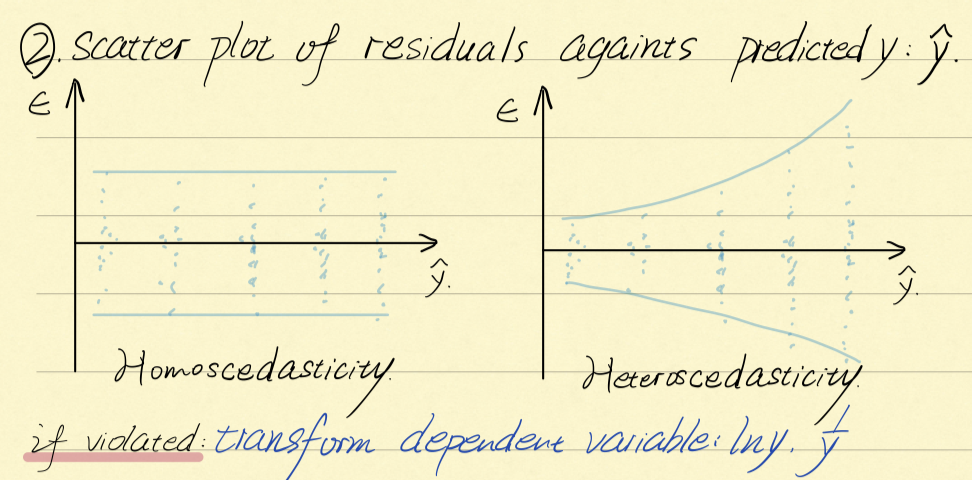
\includegraphics[scale=0.7]{check1.png}
    \caption{}
    \label{}
\end{figure}\end{center}
\textbf{MLR}:\\
If the variance is constant, the residuals will look like a football-shaped cloud. Check residual plots and look for a “fan” type shape or trends.\\
\begin{center}\begin{figure}[htbp]
    \centering
    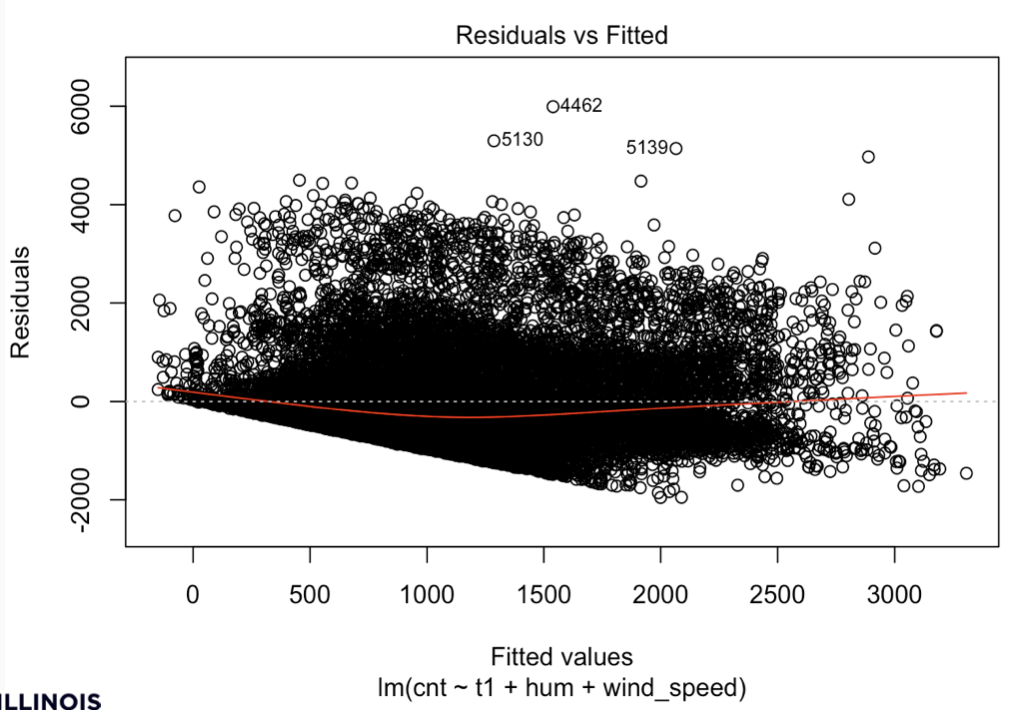
\includegraphics[scale=0.5]{check5}
    \caption{}
    \label{}
\end{figure}\end{center}


\subsubsection{Method 2: Breusch-Pagan Test}
$$\text{BP}=nR^2$$
where $R^2$ is the \textit{coefficient of Determination} between the \textbf{squared residuals} $r_i^2$ of LS regression and the \textbf{covariates} (or a sub-set) $X_1 , X_2 , . . . , X_p $.
$$
    H_0:\text{BP}\sim \chi^2_{p-1} \text{ (asymptotically)}
$$

\subsubsection{What happen if Heteroscedasticity}
\textbf{Unchanges:}\\
1. The estimaor will still be \textit{unbiased} ($\mathbb{E}(\hat{\beta})=\beta$), \textit{consistent} ($\lim_{n \rightarrow	\infty}\hat{\beta}=\beta$), but \textit{inefficient}.\\
2. Interpretation of $R^2$ is not changed.\\
\textbf{Changes:}\\
1. $\hat{\beta}$ will be \textit{inefficient}.\\
2. invalidates variance formulas for OLS estimators (${Var}(\hat{\beta}_i)$).\\
3. usual $F-$test, $t-$test are not valid.\\
4. \textit{Gauss-Markov Theorem} doesn't hold: OLS is no longer the BLUE (best linear unbiased estimator).


\subsubsection{What can we do if Heteroscedasticity}
(i) Take logarithms of each of the variables

(ii) Use suitably modified standard errors

(iii) Use a generalised least squares (GLS) procedure



\subsubsection{Remedial measure: Variance Stabilizing Transformations $\sqrt{Y}$, $\log{Y}$, $\frac{1}{Y}\text{ or }\frac{1}{Y+1}$}
\textbf{SLR}:\\
If violates Homoscedasticity: Transform \textit{dependent variable}: $\ln{y}, \frac{1}{y}$\\

\textbf{MLR}:\\
Find a transformation of the response, $h(Y )$, to achieve constant variance.\\
How does it work?\\
- Suppose $h$ is a smooth function.\\
- Using Taylor's theorem, the expansion of $h(Y)$ around $\mathrm{E}(Y)$ is:
$$
h(Y)=h(\mathbf{E}(Y))+h^{\prime}(\mathbf{E}(Y))(Y-\mathbf{E}(Y))+\text { Remainder }
$$
- The \underline{remainder} is assumed small with high probability and we can ignore it:
$$
\operatorname{Var}(\mathrm{h}(\mathrm{Y})) \approx\left(\mathrm{h}^{\prime}(\mathrm{E}(\mathrm{Y}))\right)^{2} \operatorname{Var}(\mathrm{Y})
$$
- We want to choose a transformation $h$ such that $\operatorname{Var}(\mathrm{h}(Y))$ is approximately constant.\\

\textbf{Example 1}:\\
- Suppose that the variance of $Y$ is proportional to the mean of $Y$, i.e., $\operatorname{Var}(Y) \propto E(Y)$\\
- Select $h$ such that:
$$
h^{\prime}(z)=\frac{1}{\sqrt{z}} \Rightarrow h(z) \propto \sqrt{z}
$$
- When plugging-in the value of $h^{\prime}(z)$ evaluated at $E(Y)$ in the variance of $h(Y)$ equation, the variance of $h(Y)$ will be approximately constant. Indeed,
$$
\operatorname{Var}(\sqrt{Y}) \approx\left(\frac{1}{\sqrt{E(Y)}}\right)^{2} \operatorname{Var}(Y)=\frac{\operatorname{Var}(Y)}{E(Y)} \approx \text { const }
$$\\

\textbf{Example 2}:\\
- Suppose that the variance of $Y$ is proportional to the squared mean of $Y$, i.e., $\operatorname{Var}(Y) \propto(E(Y))^{2}$.\\
- Select $h$ such that:
$$
h^{\prime}(z)=\frac{1}{z} \Rightarrow h(z)=\log (z)
$$
- Then,
$$
\operatorname{Var}(\log Y) \approx \frac{1}{(\mathrm{E}(\mathrm{Y}))^{2}} \operatorname{Var}(\mathrm{Y}) \approx \text { const }
$$\\

\textbf{Example 3:}\\
$\operatorname{Var}(Y) \propto(E(Y))^{4}$.\\
$$h(Y)=\frac{1}{Y}\text{ or }\frac{1}{Y+1}$$






\subsection{Check $2.$ Normality}
\subsubsection{Method 1: Histogram, graph $residuals$ against its frequency}
\begin{center}\begin{figure}[htbp]
    \centering
    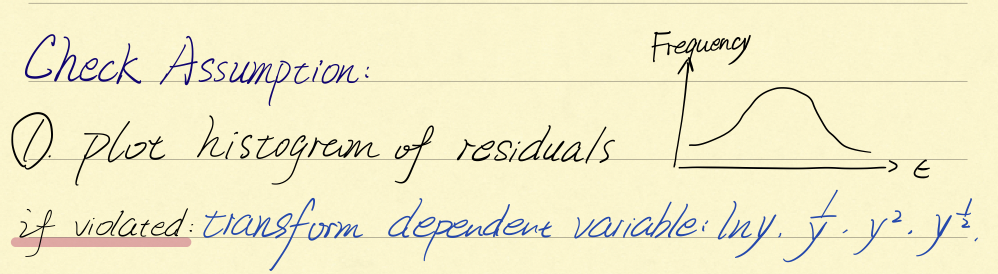
\includegraphics[scale=0.7]{check2.png}
    \caption{}
    \label{}
\end{figure}\end{center}
If violates Normality: Transform \textit{dependent variable}: $\ln{y}, \frac{1}{y},y^2,\sqrt{y}$




\subsubsection{Method 2: QQ-Plot, graph $residuals$ against its frequency}
- Suppose that we have a sample $z_{1}, z_{2}, \ldots, z_{n}$.\\
- We wish to examine the hypothesis that the z's are a sample from a normal distribution with mean $\mu$ and variance $\sigma^{2}$.\\
\textbf{QQ-Plot}:\\
1. Order the z's: $z_{(1)}, z_{(2)}, \ldots, z_{(n)}$.\\
2. Compute $u_{i}=\Phi^{-1}\left(\frac{i}{n+1}\right)$, where $\Phi$ is the cdf of the $N(0,1)$ and $i$ is the order if the data $(i=1,2, \ldots, n)$.\\
3. Plot $z_{(i)}$ against $u_{i}$.\\
$\Rightarrow$ If the z's are normal, the plot should be approximately a straight line.
\begin{center}\begin{figure}[htbp]
    \centering
    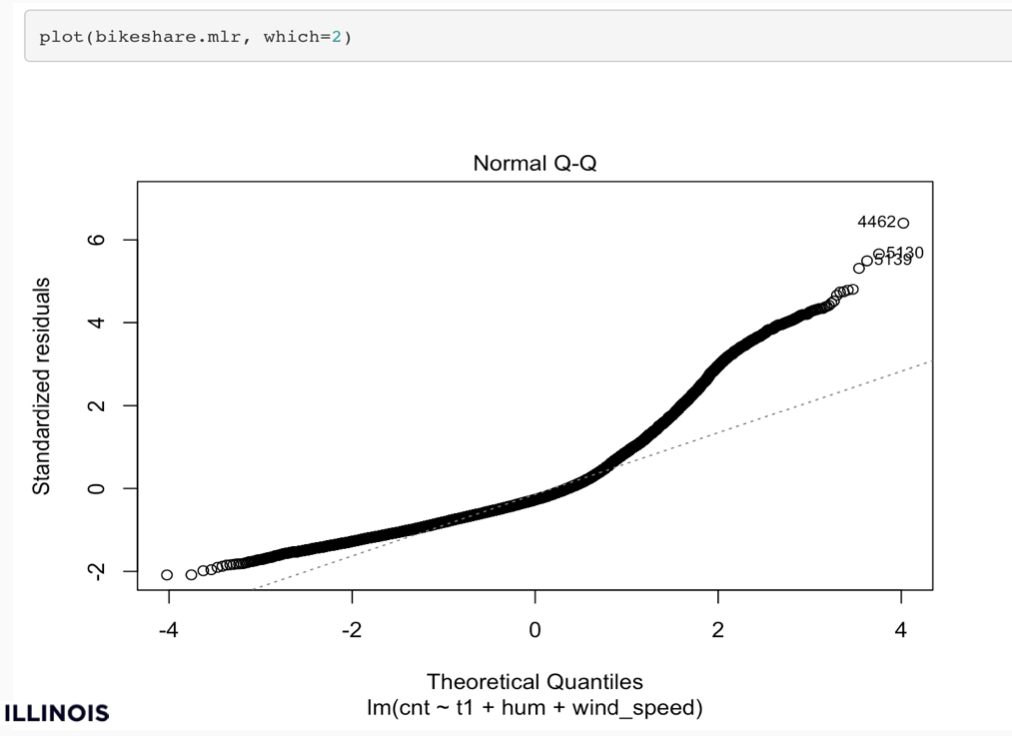
\includegraphics[scale=0.7]{check7.png}
    \caption{}
    \label{}
\end{figure}\end{center}

\subsubsection{Method 3: Shapiro-Wilk Test (good for $n \leq 50$)}
$$W=\frac{(\sum_{i=1}^n a_i r_{(i)})^2}{\sum_{i=1}^n(r_i-\bar{r})^2}$$
where $r_{(i)}$ is the $i$th largest value of the $r_i$’s and the $a_i$ terms are calculated using the means, variances, and covariances of the $r_i$s.\\
\textbf{Small values of $W$} will lead to rejection of the null hypothesis.

\subsubsection{Method 4: Kolmogorov-Smirnov Test (good for $n > 50$)}
$$D_n=\sup_x |F_n(x)-\Phi(x)|$$
where $\Phi(x)$ is the cdf of the Normal and $F_n$ the empirical distribution function $F_n$ for $n$ i.i.d. ordered observations $X_i$ is defined as
$$F_n(x)=\frac{1}{n}\sum_{i=1}^n \mathbf{1}_{[-\infty,x]}(X_i)$$
\textbf{Small values of $D$} will lead to rejection of the null hypothesis.

\subsubsection{Remedial measure: Box-Cox Transformations of $Y$}

Suppose each $y_i>0$, and consider the following transformation:
$$g_\lambda(y)=\left\{\begin{matrix}
    \frac{y^\lambda-1}{\lambda},&\lambda\neq0\\
    \log(y),& \lambda=0
\end{matrix}\right.$$
Choose $\lambda$ that maximizes the likelihood of the data, under the assumption that the transformed data $g_{\lambda}(\mathbf{y})$ has a normal distribution:
$$
g_{\lambda}(\mathbf{y})=\mathbf{X} \beta+\varepsilon, \quad \varepsilon \sim N_{n}\left(\mathbf{0}, \sigma^{2} \mathbf{l}\right)
$$
- The log-likelihood function for $\lambda \neq 0$ is:
$$
L(\lambda)=-\frac{n}{2} \log \left(R S S_{\lambda} / n\right)+(\lambda-1) \sum_{i=1}^{n} \log \left(y_{i}\right)
$$
where $R S S_{\lambda}$ is the $R S S$ when $g_{\lambda}(\mathbf{y})$ is the response, and for $\lambda=0$ is:
$$
L(0)=-\frac{n}{2} \log \left(R S S_{0} / n\right)-\sum_{i=1}^{n} \log \left(y_{i}\right)
$$
The second term in these log-likelihood function corresponds to the Jacobian of the transformation.\\

In \textbf{R}, we can graph the log-likelihood as a function of $\lambda (L(\lambda))$ versus $\lambda\in (−2, 2)$ and then pick the maximizer $\hat{\lambda}$.\\
\begin{center}\begin{figure}[htbp]
    \centering
    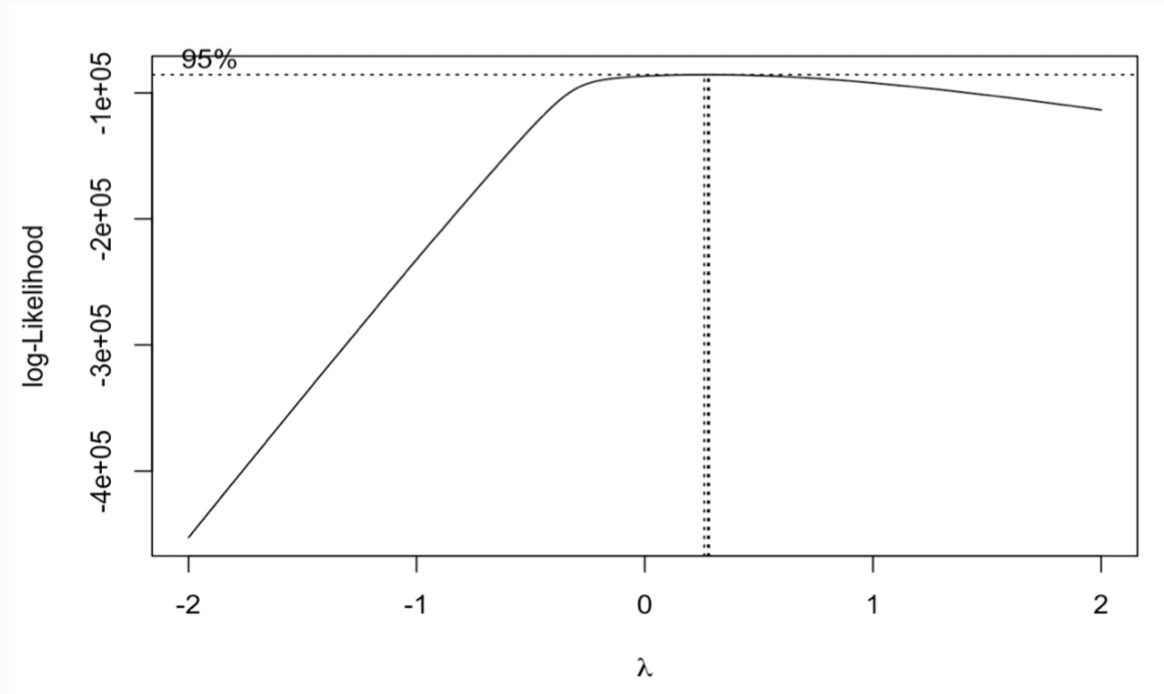
\includegraphics[scale=0.5]{check8.png}
    \caption{}
    \label{}
\end{figure}\end{center}
It is common to round $\hat{\lambda}$ to a nearby value like:
$$−1, −0.5, 0, 0.5, \text{ or } 1 $$then the transformation defined by $\hat{\lambda}$ is easier to interpret.

To answer the question whether we really need the transformation $g_\lambda$, we can do hypothesis testing $(H_0 : \lambda = 1)$, or equivalently construct a Confidence Interval for $\lambda$ as follows:
$$\{\lambda: L(\lambda)>L(\hat{\lambda})-\frac{1}{2}\chi_1^2(1-\alpha)  \}$$

















\subsection{ Checking $3.$ Serial Dependence}
\subsubsection{Method 1: graph $residuals$ against index variable(time or case number)}
\begin{center}\begin{figure}[htbp]
    \centering
    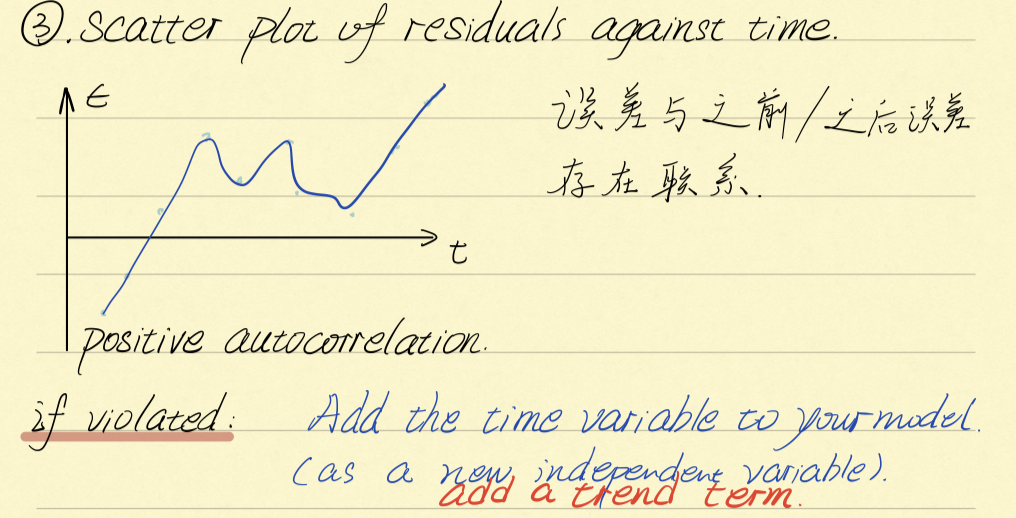
\includegraphics[scale=0.7]{check3.png}
    \caption{}
    \label{}
\end{figure}\end{center}
If violates No-Autocorrelation: add a new independent vaiable ($t$).
\subsubsection{Method 2: Durbin Watson test}
\textbf{SLR:}\\
$$d=\frac{\sum_{i=2}^n(e_i-e_{i-1})^2}{\sum_{i=1}^ne_i^2}$$
Compare $d$ with $d_L$ and $d_U$.
\begin{center}\begin{figure}[htbp]
    \centering
    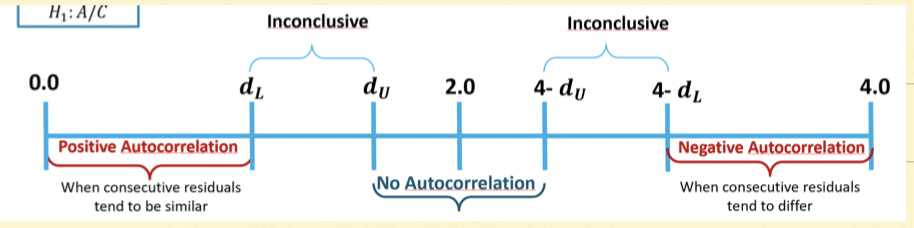
\includegraphics[scale=0.5]{check4.png}
    \caption{}
    \label{}
\end{figure}\end{center}

\textbf{MLR:}\\
$$DW=\frac{\sum_{k=1}^{n-1}(r_k-r_{k+1})^2}{\sum_{k=1}^nr_k^2}$$
if $DW<2$, then there is evidence for positive serial dependence.

\subsection{ Checking $4.$ Non-Linearity}
\subsubsection{Method 1: Partial Regression Plots}
We want to know \textbf{the relationship between the response $Y$ and a predictor $X_{k}$} after the effect of the other predictors has been removed.\\
To remove the effect of the other predictors, run the following two regression models:
\begin{equation}
    \begin{aligned}
        Y &\sim X_{1}+\ldots+X_{i-1}+X_{i+1}+\ldots &(1)\\
X_{i} &\sim X_{1}+\ldots+X_{i-1}+X_{i+1}+\ldots &(2)
    \end{aligned}
    \nonumber
\end{equation}

Get the following residuals:
$$
\begin{aligned}
\mathbf{r}_{y} &=\text { residuals from }(1) \\
\mathbf{r}_{k}^{X} &=\text { residuals from }(2)
\end{aligned}
$$
Plot $\mathbf{r}_{y}$ vs. $\mathbf{r}_{k}^{X}$ : For a valid model, the added-variable plot should produce points randomly scattered around a line through the origin with slope $\hat{\beta}_{k}$. This is also a useful plot to detect \textit{high influential} data points.

\subsubsection{Remedial measure: Linearizing Transformations}
1. $\log(Y)$ vs. $\log(X)$, suitable when $\mathbb{E}(Y)=\alpha X_1^{\beta_1}...X_p^{\beta_p}$\\
2. $\log(Y)$ vs. $X$, suitable when $\mathbb{E}(Y)=\alpha \exp{\sum_j X_j\beta_j}$\\
3. $\frac{1}{Y}$ vs. $X$, suitable when $\mathbb{E}(Y)=\frac{1}{\alpha+{\sum_j X_j\beta_j}}$

\subsubsection{Remedial measure: Box-Cox Transformations of $Y$ also works}

\section{ MLR Diagnostics: Collinearity}
\subsection{Exact Collinearity/ linearly dependent}
There exists a set of constants $c_1,c_2,...,c_p$ (at least one of them is non-zero) s.t.
$$\sum_{j=1}^pc_j \mathbf{X}_{.j}=0$$
then the columns of X are called \textit{linearly dependent} and there is \textit{exact collinearity}.

\subsection{What happens if exact collinearity}
1. $(\mathbf{X}^T \mathbf{X})^{-1}$ does not exists.\\
2. The LS estimate $\hat{\beta}$ is not unique.\\
3. The corresponding linear model is not identifiable.

\subsection{Approximate Collinearity}
We generally do not need to worry about exact collinearity ($\mathbf{R}$ can detect it and fix it automatically), but \textit{approximate collinearity}.
$$\sum_{j=1}^pc_j \mathbf{X}_{.j}\approx 0$$
$$\mathbf{X}_{.k}\approx -\sum_{j\neq k}c_j \mathbf{X}_{.j}/c_k$$
A simple diagnostic for this is to obtain the regression of $\mathbf{X}_{.k}$ on the remaining predictors, and if the corresponding $R_k^2$ is close to $1$, we would diagnose approximate collinearity.
$$\mathbf{X}_{.k}\sim \mathbf{X}_{.1}+\ldots+\mathbf{X}_{.k-1}+\mathbf{X}_{.k+1}+\ldots \Rightarrow	R_k^2$$

\subsection{What happens if approximate collinearity: based on $\left(\frac{1}{1-R_{k}^{2}}\right)$ ($k-$th variance inflation factor (VIF), $VIF>10$)}
In a multiple regression $Y=\beta_{0}+\beta_{1} X_{1}+\ldots+\beta_{p} X_{p}+e$, the LS estimate $\hat{\beta}_{k}$ is unbiased with variance:
$$
\operatorname{Var}\left(\hat{\beta}_{\mathrm{k}}\right)=\sigma^{2}\left(\frac{1}{1-\mathrm{R}_{\mathrm{k}}^{2}}\right)\left(\frac{1}{\sum_{\mathrm{i}=1}^{n}\left(\mathrm{x}_{\mathrm{ik}}-\overline{\mathrm{x}}_{\cdot \mathrm{k}}\right)^{2}}\right)
$$
where $R_{k}^{2}$ is the R-square from the regression of $\mathbf{X}_{\cdot k}$ on the remaining predictors. When $R_{k}^{2}$ is close to 1 , the variance of $\hat{\beta}_{k}$ is large.\\
Consequently we will have:\\
1. large Mean Square Error\\
2. large (inflated) $p$-value to the corresponding $t$-test, i.e, we could miss a significant predictor.\\
The quantity $\left(\frac{1}{1-R_{k}^{2}}\right)$ is called the $k$-th variance inflation factor (VIF).\\
${VIF}>10$ infers conllinearity

\subsection{Possible symptoms of collinearity}
1. high pair-wise (sample) correlation between predictors\\
2. high VIF\\
3. high condition number\\
4. $R^2$ is relatively large but none of the predictor is significant.

\subsection{Global Measure of Collinearity: \textit{condition number} of $\mathbf{X}^T \mathbf{X}$}
\textit{Condition number} of $\mathbf{X}^T \mathbf{X}$:
$$\kappa=(\text{largest eigenvalue/smallest eigenvalue})^{1/2}$$
An empirical rule for declaring collinearity is $\kappa\geq 30$\\
Note that $\kappa$ is \textit{not scale-invariant}, so we should \textit{standardized} each column of $X$ (i.e. each column should have \textit{zero mean} and \textit{sample variance} equal to $1$, before calculating the condition number).

\subsection{What to do with collinearity}
1. Remove some predictors from highly correlated groups of predictors.\\
2. Regularize the model using penalized Least Squares estimation.





\section{Generalized Least Squares (GLS)}
What do we do if the errors are \textbf{correlated} or \textbf{heteroscedastic}?\\
Suppose $\varepsilon \sim \mathcal{N}_{n}(0, \Sigma)$, where $\Sigma$ is the variance-covariance matrix.
\subsection{GLS, $\Sigma$ known ($\hat{\beta}=\left(\mathbf{X}^{\top} \Sigma^{-1} \mathbf{X}\right)^{-1} \mathbf{X}^{\top} \Sigma^{-1} \mathbf{y}$, ${RSS}=(\mathbf{y}-\mathbf{X} \beta)^{\top} \Sigma^{-1}(\mathbf{y}-\mathbf{X} \beta)$)}
\subsubsection{Method 1: Transform back to OLS}
$$
\mathbf{y}=\mathbf{X} \beta+\varepsilon
$$
where $\varepsilon \sim \mathcal{N}_{n}(0, \Sigma)$ and $\Sigma$ is a known, symmetric, positive definite covariance matrix.\\
When the errors are heteroscedastic or correlated:\\
Transform this problem back to Ordinary Least-Squares (OLS):\\
1. Assume $S^{-1}$ exists and write
$$
\Sigma=S S^{\top}
$$
(We could use, for example, the Cholesky decomposition from linear algebra to obtain $S$.)\\

2. Multiply the model equation by $S^{−1}$ on both sides:
$$
\begin{aligned}
\mathbf{y} &=\mathbf{X} \beta+\varepsilon \\
S^{-1} \mathbf{y} &=S^{-1}(\mathbf{X} \beta+\varepsilon) \\
\underbrace{S^{-1} \mathbf{y}}_{:=\mathbf{y}^{*}} &=\underbrace{S^{-1} \mathbf{X}}_{:=\mathbf{x}^{*}} \beta+\underbrace{S^{-1} \varepsilon}_{:=\varepsilon^{*}} \\
\mathbf{y}^{*} &=\mathbf{X}^{*} \beta+\varepsilon^{*}
\end{aligned}
$$
This implies that
$$
\varepsilon^{*} \sim \mathcal{N}(S^{-1} \mathbf{0}, \underbrace{S^{-1} \Sigma\left(S^{-1}\right)^{\top}}_{=\text {ldentity }})=\mathcal{N}(\mathbf{0}, \mathbf{I})
$$
since $S^{-1} \Sigma\left(S^{-1}\right)^{\top}=S^{-1} S S^{\top}\left(S^{-1}\right)^{\top}=I$\\

3. For the transformed model, we can solve for $\beta$ using OLS:
$$
\mathbf{y}^{*}=\mathbf{X}^{*} \beta+\varepsilon^{*}
$$
where $\mathbf{y}^{*}=S^{-1} \mathbf{y}, \mathbf{X}^{*}=S^{-1} \mathbf{X}$\\
So, the estimator for $\beta$ computes as
$$
\begin{aligned}
\hat{\beta} &=\left(\mathbf{X}^{* \top} \mathbf{X}^{*}\right)^{-1} \mathbf{X}^{* \top} \mathbf{y}^{*} \\
&=(\mathbf{X}^{\top} \underbrace{\left(S^{-1}\right)^{\top} S^{-1}}_{=\Sigma^{-1}} \mathbf{X})^{-1} \mathbf{X}^{\top} \underbrace{\left(S^{-1}\right)^{\top} S^{-1}}_{=\Sigma^{-1}} \mathbf{y} \\
&=\left(\mathbf{X}^{\top} \Sigma^{-1} \mathbf{X}\right)^{-1} \mathbf{X}^{\top} \Sigma^{-1} \mathbf{y}
\end{aligned}
$$
Note that the solution we obtained minimizes:
$$
\left\|\mathbf{y}^{*}-\mathbf{X}^{*} \beta\right\|^{2}=(\mathbf{y}-\mathbf{X} \beta)^{\top} \Sigma^{-1}(\mathbf{y}-\mathbf{X} \beta)
$$

\subsubsection{Weighted Least Squares (WLS)}
Suppose that $\Sigma$ is a diagonal matrix of unequal error variances:
$$
\Sigma=\operatorname{diag}\left(\sigma_{1}^{2}, \sigma_{2}^{2}, \ldots, \sigma_{n}^{2}\right)
$$
The GLS estimate of $\beta$ minimizes:
$$
(\mathbf{y}-\mathbf{X} \beta)^{\top} \Sigma^{-1}(\mathbf{y}-\mathbf{X} \beta)=\sum_{i=1}^{n} \frac{\left(y_{i}-\mathbf{x}_{i}^{\top} \beta\right)^{2}}{\sigma_{i}^{2}}
$$
This problem is known as the Weighted Least-Squares (WLS).\\
Note that the errors are weighted by
$$
w_{i}=\frac{1}{\sigma_{i}^{2}}
$$
smaller weights for samples with larger variances.

\subsubsection{WLS special example : Replicated Observations}
Suppose we collected multiple observations for each $\mathbf{x}_{i}$. We use double subscripts to indicate the replicate observations:
$$
\left(\mathbf{x}_{i}, y_{i 1}, y_{i 2}, \ldots, y_{i n_{i}}\right)
$$
Let $y_{i}$ denote the average of the $n_{i}$ observations sharing $\mathbf{x}_{i}$. Then the residual sum of squares for $\beta$ equals
$$
\sum_{i=1}^{n} \sum_{j=1}^{n_{i}}\left(y_{i j}-\mathbf{x}_{i}^{\top} \beta\right)^{2}=\sum_{i=1}^{n} n_{i}\left(y_{i}-\mathbf{x}_{i}^{\top} \beta\right)^{2}+\sum_{i=1}^{n} \sum_{j=1}^{n_{i}}\left(y_{i j}-y_{i}\right)^{2}
$$
Minimizing the $RSS$ to solve for $\beta$ is the same as minimizing the first term on the right only.
$$\hat{\beta}=\argmin_\beta \sum_{i=1}^n n_i(y_i-\mathbf{x}_i^T\beta)^2$$

\subsubsection{Method 2: Likelihood Estimation}
Model: $\mathbf{y} \sim N_{n}(\mathbf{X} \beta, \Sigma)$\\
Log-likelihood:
$$
\begin{aligned}
&\log (p(\mathbf{y} \mid \beta, \Sigma)) \\
&\quad=\log \left\{\frac{1}{(2 \pi)^{n / 2}|\Sigma|^{1 / 2}} \exp \left[-\frac{1}{2}(\mathbf{y}-\mathbf{X} \beta)^{\top} \Sigma^{-1}(\mathbf{y}-\mathbf{X} \beta)\right]\right\} \\
&\quad=-\frac{1}{2}(\mathbf{y}-\mathbf{X} \beta)^{\top} \boldsymbol{\Sigma}^{-1}(\mathbf{y}-\mathbf{X} \beta)+\text { Constant. }
\end{aligned}
$$
Therefore the MLE is given by
$$
\hat{\beta}_{m l e}=\arg \min _{\beta}(\mathbf{y}-\mathbf{X} \beta)^{\top} \Sigma^{-1}(\mathbf{y}-\mathbf{X} \beta)
$$

\subsection{GLS, $\Sigma$ unknown}
\subsubsection{Method 1: Estimation of Variance ($r_i^2$)/Standard Deviation Function ($|r_i|$)}
$$\sigma_i^2=\mathbb{E}(\varepsilon_i^2)-(\mathbb{E}(\varepsilon_i))^2$$
Since we assume $E(\varepsilon_i)=0$, we have
$$\sigma_i^2=\mathbb{E}(\varepsilon_i^2)$$
Which implies $r_i^2$ is an estimator of $\sigma_i^2$; $|r_i|$ is an estimator of the standard deviation $\sigma_i$.\\

\textbf{Estimate Variance Function} $\hat{v_i}(x)$

1. Fit a regression model using OLS, and obtain the residuals $r_i$.\\
2. Regress the squared residuals $r_i^2$ against the appropriate predictor variables.\\
Denote $\hat{v_i}$ be the fitted value from variance function
$$w_i=\frac{1}{\hat{v_i}}$$

\textbf{Estimate Standard Deviation Function} $\hat{s_i}(x)$

1. Fit a regression model using OLS, and obtain the residuals $r_i$.\\
2. Regress the absolute residuals $|r_i|$ against the appropriate predictor variables.\\
Denote $\hat{s_i}$ be the fitted value from standard deviation function
$$w_i=\frac{1}{(\hat{s_i})^2}$$
The estimated variances are then placed in the variance-covariance matrix $\Sigma$ and the regression coefficients are estimated using the WLS (Weighted Least Squares method).

\subsubsection{Method 2: iterative approach}
1. Start with some initial guess of $\Sigma$\\
2. Use $\Sigma$ to estimate $\beta$\\
3. Use residuals (since we have known $\beta$) to estimate $\Sigma$\\
4. Iterate until convergence.\\

It looks like a good idea; however the methods will not work if we do not assume some structure about $\Sigma$ (too many parameters to be estimated).

Based on the application, we can assume a particular structure for $\Sigma$ that does not involve too many parameters.\\
Then, we can model $\beta$ and $\Sigma$ simultaneously.\\
For example , for AR(1) times series (auto-regressive model of order 1),
the structure of $\Sigma$ would be:
$$\Sigma=\sigma^2 \begin{pmatrix}
    1& \rho& \rho^2& \rho^3& \cdots\\
    \rho& 1& \rho& \rho^2& \cdots \\
    \cdots & \cdots& \cdots &\cdots&\cdots \\
    \rho^{n-1}& \rho^{n-2}&\cdots&\cdots&1
\end{pmatrix}$$
$\Sigma$ as a function of $\rho$ and $\sigma^2$.

\section{ GLS Diagnostics: Lack of Fit Tests}
\subsection{Gaussian Assumption}
Gaussian Assumption, which can be summarized concisely as:
$$y\sim \mathcal{N}_{n}(\mathbf{X}\beta, \sigma^2 \mathbf{I})$$
Under these assumptions:
\begin{equation}
    \begin{aligned}
        \hat{\beta}&=\left(\mathbf{X}^{T} \mathbf{X}\right)^{-1} \mathbf{X}^{T} y\sim \mathcal{N}_{p}(\beta,\sigma^2\left(\mathbf{X}^{T} \mathbf{X}\right)^{-1}),\\
        \hat{y}&=\mathbf{X}\hat{\beta}\sim \mathcal{N}_{n}(\mathbf{X}\beta, \sigma^2 \mathbf{H})
    \end{aligned}
    \nonumber
\end{equation}
independently,
$$\hat{\sigma}^2=\frac{RSS}{n-p}=\frac{||y-\hat{y}||^2}{n-p}\sim \sigma^2\frac{\chi^2_{n-p}}{n-p}$$

\subsection{When $\sigma^2$ is known}
Intuition:\\
If the model is correct, then $\hat{\sigma}^2$ is an unbiased estimate of $\sigma^2$.\\
If we know $\sigma^2$, we could construct a test based on the ratio $\frac{\hat{\sigma}^2}{\sigma^2}$, a measure of \textit{lack-of-fit}.

In this case we want to test the hypothesis:
$$
\left\{\begin{array}{l}
H_{0}: \text { There is no lack of fit. } \\
H_{\alpha}: \text { There is lack of fit. }
\end{array}\right.
$$
We use the test statistic:
$$
\frac{\hat{\sigma}^{2}}{\sigma^{2}}=\frac{R S S /(n-p)}{\sigma^{2}} \sim \frac{\chi_{n-p}^{2}}{n-p}
$$
Lack of fit means the error variance is large related to the value of $\sigma^{2}$, i.e., the test statistic is large.\\
Conclude that there is lack of fit (i.e. Reject $\left.H_{0}\right)$, if:
$$
(n-p) \frac{\hat{\sigma}^{2}}{\sigma^{2}} \geq \chi_{n-p}^{2}(1-\alpha)
$$

\subsection{When $\sigma^2$ is unknown}
\subsubsection{Hypothesis}
If $\sigma^{2}$ is unknown, a general approach is to compare an estimate of $\sigma^{2}$ based on a \underline{much bigger/general model}.\\
If we can derive the distribution (under $\mathrm{H}_{0}$ ) of $\hat{\sigma}_{\text {LinearModel }}^{2} / \hat{\sigma}_{\text {BigModel }}^{2}$, then we reduce this problem to a two model comparison test problem.\\
The null hypothesis is the current model:\\
$H_{0}: \mathbb{E}\left(y_{i}\right)=\mathbf{x}_{i}^{\top} \beta, \quad i=1,2, \ldots, n, \quad$ for some vector $\beta$\\
The more general model is assumed under the alternative hypothesis:\\
$H_{\alpha}: \mathbb{E}\left(y_{i}\right)=f\left(\mathbf{x}_{i}\right), \quad i=1,2, \ldots, n$, \quad for some function $f$\\

\subsubsection{Under the null hypothesis $H_{0}$}
$y_{i j}=\mathbf{x}_{i}^{\top} \beta+\varepsilon_{i j}$, some $\beta, \varepsilon_{i j} \sim$ iid $\mathcal{N}\left(0, \sigma^{2}\right)$\\
$R S S_{0}$ with $d f=n-p$
\subsubsection{Under the alternative big-model hypothesis $H_{\alpha}$ :}
$y_{i j}=f\left(\mathbf{x}_{i}\right)+\varepsilon_{i j}$, some function $f, \varepsilon_{i j} \sim$ iid $\mathcal{N}\left(0, \sigma^{2}\right)$\\
\textbf{Can we estimate $\sigma^{2}$ for the big model in $H_{\alpha}$ ?}\\
- The answer is yes, if there is some replication in the data, i.e., there are multiple observations (replicates) for some (at least) of the same $\mathbf{x}_{i}$ values.\\
- Schematically we can represent these replicates as:
$$
\left(\mathbf{x}_{i}, y_{i 1}, y_{i 2}, \ldots, y_{i n_{i}}\right), \quad i=1: m, \quad n=\sum_{i} n_{i}
$$
$R S S_{a}$ with $d f=n-m=\sum_{i}\left(n_{i}-1\right)$, where
$$
R S S_{a}=\sum_{i=1}^{m} \sum_{j=1}^{n_{i}}\left(y_{i j}-\bar{y}_{i .}\right)^{2}
$$
\subsubsection{$F-$Test}
All of the degrees of freedom for $R S S_{a}$ come from the replications. Therefore, with replication we can do an $\mathrm{F}$ test for lack of fit:
$$
F=\frac{\left(R S S_{0}-R S S_{a}\right) /(m-p)}{R S S_{a} /(n-m)} \sim F_{m-p, n-m}
$$

\section{Polynomials Regression}
\subsection{Basic Function}
\begin{equation}
    \begin{aligned}
        y_i&=f(x_i)+\varepsilon_i\\
        y_i&=\beta_0+\sum_{j=1}^db_j(x_i)\beta_j+\varepsilon_i\\
        y_i&=\beta_0+\sum_{j=1}^d\beta_j
        x_i^j+\varepsilon_i\\
    \end{aligned}
    \nonumber
\end{equation}
$d$ is the \textbf{degree of the polynomial component}.\\
\subsection{Choose Order $d$}
1.\textbf{Forward Approach}: Keep adding terms until the last added term is not significant.\\
2.\textbf{Backward Approach}: Start with a large $d$, and keep eliminating the terms that are not statistically significant, starting with the highest order term.\\

Once we pick up a $d$, we do not test the significance of the lower-order terms. (include all the lower-order terms in our model by default)\\
\textbf{Reasoning}: we do not want our results to be affected by a change of location/scale of the data. $(z_i-2)^2=z_i^2-4z_i+4$.\\
\textbf{Exception}: particular polynomial function (physics law).


\subsection{Orthogonal Polynomials}
Successive predictors $x^j$ are \textbf{highly correlated} introducing multicollinearity problems.
\begin{equation}
    \begin{aligned}
        y_i=\beta_0+\beta_1 \mathbf{z}_i+...+\beta_d \mathbf{z}_d+\varepsilon_i
    \end{aligned}
    \nonumber
\end{equation}
where $\mathbf{z}_j=a_1+b_2x+...+\kappa_j x^j$ is a polynomial of order $j$ with coefficients chosen such that $\mathbf{z}_j^T\mathbf{z}_j=0$

\subsection{Piece-wise Polynomials}
If the true mean of $E(Y | X = x) = f (x)$ is too wiggly, we might need to fit a higher order polynomial, which is not always a good idea.\\

Instead we will consider \textbf{piece-wise polynomials}:

1.we divide the range of $x$ into several intervals, and

2.within each interval $f (x)$ is a low-order polynomial, e.g., cubic or quadratic, but the polynomial coefficients change from interval to interval;

3.in addition we require the overall $f (x)$ to be continuous up to certain derivatives.

\subsection{Cubic Splines}
\subsubsection{Why Spline}
\textbf{Polynomials}: smooth, but each point affects the fit globally.\\
\textbf{Piece-wise Polynomials}: localizes the influence of each data point, but are not smooth enough.\\
\textbf{Splines}: combines the beneficail aspects of both approaches.\\

\subsubsection{Settings}
A \textbf{Cubic Spline} is a curve constructed from sections of cubic polynomials, joined together so that the curve is \textit{continuous up to second derivative}.\\
The points at which the sections join are called the \textbf{knots} of the spline.\\

We want to define a cubic spline function in the interval $[a, b]$\\
- Define $m$ knots such that: $a<\xi_{1}<\xi_{2}<\ldots<\xi_{m}<b$\\
- A function $g$ defined on $[a, b]$ is a \textbf{cubic spline with respect to knots $\left\{\xi_{i}\right\}_{i=1}^{m}$} if:\\
1. $g$ is a cubic polynomial in each of the $m+1$ intervals,
$$
g(x)=d_{i} x^{3}+c_{i} x^{2}+b_{i} x+a_{i}, \quad x \in\left[\xi_{i}, \xi_{i+1}\right]
$$
where $i=0, \ldots, m, \xi_{0}=a$ and $\xi_{m+1}=b$\\
2. $g$ is continuous up to the 2 nd derivative: since $g$ is continuous up to the 2nd derivative for any point inside an interval, it suffices to check the following conditions:
$$
g^{(0,1,2)}\left(\xi_{i}^{+}\right)=g^{(0,1,2)}\left(\xi_{i}^{-}\right), \quad i=1: m
$$
This expression indicates that the function and the first and second order derivatives are continuous at the knots.\\

\subsubsection{Number of free parameters: $m+4$}
How many free parameters do we need to represent a cubic spline?\\
(i) 4 parameters $\left(d_{i}, c_{i}, b_{i}, a_{i}\right)$ for each of the $(m+1)$ intervals.\\
(ii) 3 constraints at each of the $m$ knots (continuity constraints).\\
The \textbf{total number of free parameters} (similar to the number of degrees of freedom) is:
$$
4(m+1)-3 m=m+4
$$

\subsubsection{Properties: linear combination also cubic spline}
Given knots $\{\xi_i\}_{i=1}^m$, the linear combinations of cubic splines are also cubic splines.\\
That is, for a set of given knots, the corresponding cubic splines form a linear space (of functions) with ${dim} (m + 4)$.

\subsubsection{Cubic Splines Basis}
A set of basis functions for cubic splines (w.r.t knots $\left\{\xi_{i}\right\}_{i=1}^{m}$ ) is given by:
$$
\begin{aligned}
h_{0}(x) &=1 \\
h_{1}(x) &=x \\
h_{2}(x) &=x^{2} \\
h_{3}(x) &=x^{3} \\
h_{i+3}(x) &=\left(x-\xi_{i}\right)_{+}^{3}, \quad i=1,2, \ldots, m
\end{aligned}
$$
That is, any cubic spline can be uniquely expressed as:
$$
\beta_{0}+\sum_{j=1}^{m+3} \beta_{j} h_{j}(x)
$$
Given knot locations, there are many alternative, but equivalent ways of writing down a basis for cubic splines.
\begin{example}[Other Basis]
    For example, another basis for cubic splines can be the following:
    $$
    \begin{aligned}
    h_{0}(x) &=1 \\
    h_{1}(x) &=x \\
    h_{i+1}(x) &=R\left(x, \xi_{i}^{*}\right), i=1, \ldots, q-1
    \end{aligned}
    $$
    where
    $$
    \begin{aligned}
    R(x, z)=&\left[(z-1 / 2)^{2}-1 / 12\right]\left[(x-1 / 2)^{2}-1 / 12\right] / 4 \\
    &-\left[(|x-z|-1 / 2)^{4}-1 / 2(|x-z|-1 / 2)^{2}+7 / 240\right] / 24
    \end{aligned}
    $$
\end{example}

\subsection{Natural Cubic Splines (NCS)}
A cubic spline on $[a, b]$ is a \textbf{Natural Cubic Spline} if its \textit{second and third derivatives are zero at a and $b$}.
\subsubsection{Degree of Freedom (Number of free parameters): $m$}
This condition implies that NCS is a linear function in the two extreme intervals $\left[a, \xi_{1}\right]$ and $\left[\xi_{m}, b\right]$. The linear functions in the two extreme intervals are completely determined by their neighboring intervals.\\
The degree of freedom of NCS's with $m$ knots is:
$$
4(m+1)-3 m-4=m
$$
(We have 4 additional constraints.)

\subsubsection{NCS Basis}
A Natural Cubic Spline with $m$ knots is represented by $m$ basis functions, for example, one such basis is given by
$$
\begin{aligned}
N_{1}(x) &=1 \\
N_{2}(x) &=x \\
N_{k+2}(x) &=d_{k}(x)-d_{k-1}(x)
\end{aligned}
$$
where
$$
d_{k}(x)=\frac{\left(x-\xi_{k}\right)_{+}^{3}-\left(x-\xi_{m}\right)_{+}^{3}}{\xi_{m}-\xi_{k}}
$$
Each of these derivatives can be seen to have zero second and third derivative for $x \geq \xi_{m}$.

\subsubsection{Note: Waste of Data points}
Recall that the \textbf{linear functions} in the two extreme intervals are completely determined by the other cubic splines. So data points in the two extreme intervals (i.e., outside the two boundary knots) are wasted since they do not affect the fitting.\\











\subsection{Regression Splines}
We can represent the model on the observed $n$ data points using matrix notation:
$$
\left(\begin{array}{l}
y_{1} \\
y_{2} \\
\ldots \\
y_{n}
\end{array}\right)_{n \times 1}=\left(\begin{array}{llll}
h_{0}\left(x_{1}\right) & h_{1}\left(x_{1}\right) & \ldots & h_{p-1}\left(x_{1}\right) \\
h_{0}\left(x_{2}\right) & h_{1}\left(x_{2}\right) & \ldots & h_{p-1}\left(x_{2}\right) \\
&&\ldots&\\
h_{0}\left(x_{n}\right) & h_{1}\left(x_{n}\right) & \ldots & h_{p-1}\left(x_{n}\right)
\end{array}\right)_{n \times p}\left(\begin{array}{l}
\beta_{1} \\
\beta_{2} \\
\ldots \\
\beta_{p}
\end{array}\right)_{p \times 1}
$$
where our design matrix is the matrix $\mathbf{F}$ of basis functions.\\
We can find $\beta$ by solving the problem:
$$
\hat{\beta}=\arg \min _{\beta}\|\mathbf{y}-\mathbf{F} \beta\|^{2}
$$

\subsection{$K-$Fold Cross-Validation}
\begin{center}
    How to select the optimal number of knots (or df)?
\end{center}
\textbf{K-Fold Cross-Validation} Steps:\\
1. Set a fixed number of knots (or df).

2. Divide the set of observations into k groups (or folds).

3. Leave the first fold as a validation set (not used to fit the model). Fit the Regression Spline with a fixed number of knots using the remaining k − 1 folds.

4. Calculate the \textit{Mean Square Error} for fold 1: ${MSE}_1$.

5. Repeat the previous steps k times. Each time a new validation set is used to calculate ${MSE}_i$.

6. Calculate the average k-fold \textit{Cross-Validation error}: $${CV}(k) = \frac{1}{k} \sum_{i=1}^{k}{MSE}_i$$

7. Repeat 2 to 6 with a new number of knots (or df).

8. Select the number of knots that \textbf{minimizes} the k-fold ${CV}$ error or ${CV}(k)$.







\section{ANOVA: ANalysis of COVAriance: Basic}
These are regression problems where some predictors are quantitative (i.e. numerical) and some are qualitative (i.e. categorical).
\subsection{Two level example}
For simplicity, we will focus on examples with just two predictors:
$X$ (numerical) and $D$ (categorical).\\
$D$ has two levels: 0 or 1.\\
\textbf{General Model}
\begin{equation}
    \begin{aligned}
        y = \beta_0 + \beta_1 x + \beta_2 d + \beta_3 (x\cdot d) + \varepsilon
    \end{aligned}
    \nonumber
\end{equation}
\textbf{Model 1: Coincident regression lines}
\begin{equation}
    \begin{aligned}
        y = \beta_0 + \beta_1 x + \varepsilon
    \end{aligned}
    \nonumber
\end{equation}
\textbf{Model 1'}
\begin{equation}
    \begin{aligned}
        y = \beta_0 + \beta_2 d  + \varepsilon
    \end{aligned}
    \nonumber
\end{equation}
\textbf{Model 2: Parallel regression lines}
\begin{equation}
    \begin{aligned}
        y = \beta_0 + \beta_1 x+ \beta_2 d + \varepsilon
    \end{aligned}
    \nonumber
\end{equation}
\textbf{Model 3: Regression lines with equal intercepts but different slopes}
\begin{equation}
    \begin{aligned}
        y = \beta_0 + \beta_1 x + \beta_3 (x\cdot d) + \varepsilon
    \end{aligned}
    \nonumber
\end{equation}
\textbf{Model 4: Unrelated regression lines}
\begin{equation}
    \begin{aligned}
        y = \beta_0 + \beta_1 x + \beta_2 d + \beta_3 (x\cdot d) + \varepsilon
    \end{aligned}
    \nonumber
\end{equation}
\textbf{Hierarchical Rule} for interactions:
\textit{an interaction term will be included in a model only if all its main effects have been included.}\\
Due to this rule, we would include both $\beta_1$ and $\beta_2$, once $\beta_3$ is significant. So, we don't consider model 3 this place.\\
\subsection{Two-level Test: t-test}
\textbf{Which model to pick?}\\
1. test whether the interaction term is significant:
\begin{equation}
    \begin{aligned}
        H_0 : \text{model 2}\quad H_\alpha : \text{model 4}
    \end{aligned}
    \nonumber
\end{equation}
2. if don't reject $H_0$, test whether you can further reduce model 2 to model 1
\begin{equation}
    \begin{aligned}
        H_0 : \text{model 1}\quad H_\alpha : \text{model 2}
    \end{aligned}
    \nonumber
\end{equation}

\subsection{Multi-level example}
Model the response $Y$ by two predictors $X$ and $D$, where $X$ is a numerical variable and $D$ is categorical with $k$ levels.\\
We need to generate $k-1$ dummy variables: $D_{2}, \ldots, D_{k}$ where:
$$
D_{i}= \begin{cases}0, & \text { if not level } \mathrm{i} \\ 1, & \text { if level } \mathrm{i}\end{cases}
$$
Level 1 is the reference level.\\
\textbf{Model 0}: $Y\sim  1$\\
\textbf{Model 1}: $Y\sim  X$\\
\textbf{Model 1'}: $Y\sim  D$\\
\textbf{Model 2}: $Y\sim  D+X$\\
\textbf{Model 4}: $Y\sim  D+X+D:X$\\

\subsection{Multi-level Test: F-test}
Note that when $D$ has more than two levels, the difference between model parameter number may not be one, so t-test is no longer appropriate.\\
1) Compare models:
$$
H_{0}: Y \sim X+D \quad \text { vs. } \quad H_{\alpha}: Y \sim D+X+D: X
$$
If the interaction $D: X$ is significant, stop.\\
2) If $X$ is significant, keep $X$.\\
$2^{\prime}$) If $D$ is significant, keep $D$.\\
3) If neither $X$ nor $D$ are significant, report the intercept model $Y \sim 1$\\

\textbf{Sequential ANOVA}
We can use the anova function to get sequential F-tests. The sequence of $F$ -tests given by anova $(\operatorname{lm}(Y \sim X+D+X: D))$
\begin{center}
    \begin{tabular}{|c|c|}
        \hline$H_{0}$ & $H_{\alpha}$ \\
        \hline \hline$Y \sim 1$ & $Y \sim X$ \\
        $Y \sim X$ & $Y \sim X+D$ \\
        $Y \sim X+D$ & $Y \sim X+D+X: D$ \\
        \hline
        \end{tabular}
\end{center}
The sequence of $F$ -tests given by anova $(\operatorname{lm}(Y \sim D+X+X: D))$
\begin{center}
\begin{tabular}{|c|c|}
\hline$H_{0}$ & $H_{\alpha}$ \\
\hline \hline$Y \sim 1$ & $Y \sim D$ \\
$Y \sim D$ & $Y \sim D+X$ \\
$Y \sim D+X$ & $Y \sim D+X+X: D$ \\
\hline
\end{tabular}
\end{center}
\textbf{Note}: Some of the F-stats and p-values from the sequential ANOVA table are \textbf{different} from the ones we calculated based on usual F-test (we learned) for comparing two nested models.\\
Suppose we want to compare:
$$
H_{0}: Y \sim X \quad \text { vs } \quad H_{\alpha}: Y \sim X+D
$$
The usual $F$-stat is given by:
$$
\frac{\left(R S S_{0}-R S S_{a}\right) /(k-1)}{R S S_{a} /\left(n-p_{a}\right)}=\frac{\left(R S S_{0}-R S S_{a}\right) /(k-1)}{\hat{\sigma}_{a}^{2}}
$$
which follows $F_{k-1, n-p_{a}}$ under the null hypothesis. $k$ is the total number of categories of variable $D$\\
The $F$-stat from the sequential ANOVA table:
$$
\frac{\left(R S S_{0}-R S S_{a}\right) /(k-1)}{R S S_{A} /\left(n-p_{A}\right)}=\frac{\left(R S S_{0}-R S S_{a}\right) /(k-1)}{\hat{\sigma}_{A}^{2}}
$$
which follows $F_{k-1, n-p_{A}}$ under the null hypothesis, where $R S S_{A}$ denotes the RSS from the biggest model $Y \sim X+D+X: D$ and $p_{A}=2 k$


\section{Variable Selection}
\subsection{ Training and Test Errors}
Training data: $\left(\mathbf{x}_{i}, y_{i}\right)_{i=1}^{n}$\\
Test data: $\left(\mathbf{x}_{i}, y_{i}^{*}\right)_{i=1}^{n}$ is an independent (imaginary) data set collected at the same location $\mathbf{x}_{i}$ 's (also known as in-sample prediction)\\
Assume the data comes from a linear model:\\
$\mathbf{y}_{n \times 1,} \mathbf{y}_{n \times 1}^{*}$ are i.i.d $\sim N_{n}\left(\mu, \sigma^{2} \mathbf{I}_{n}\right)$ and $\mu=\mathbf{X} \beta$\\
We can also write:
$$
\begin{aligned}
\mathbf{y} &=\mathbf{X} \beta+\varepsilon \\
\mathbf{y}^{*} &=\mathbf{X} \beta+\varepsilon^{*}
\end{aligned}
$$
with $\varepsilon_{n \times 1}, \varepsilon_{n \times 1}^{*} \quad$ i.i.d $\sim \mathcal{N}_{n}\left(\mathbf{0}, \sigma^{2} \mathbf{I}_{n}\right)$ are independent.\\

$\begin{aligned} \mathbb{E}(\text { Test Error })^{2} &=\mathbb{E}\left\|\mathbf{y}^{*}-\mathbf{X} \hat{\beta}\right\|^{2} \\ &=\mathbb{E}\left\|\left(\mathbf{y}^{*}-\mathbf{X} \beta\right)+(\mathbf{X} \beta-\mathbf{X} \hat{\beta})\right\|^{2} \\ &=\mathbb{E}\left\|\mathbf{y}^{*}-\mu\right\|^{2}+\mathbb{E}\|\mathbf{X} \beta-\mathbf{X} \hat{\beta}\|^{2} \\ &=\mathbb{E}\left\|\varepsilon^{*}\right\|^{2}+\operatorname{Tr}\left(\mathbf{X} \operatorname{Cov}(\hat{\beta}) \mathbf{X}^{\top}\right) \\ &=n \cdot \sigma^{2}+\sigma^{2} \operatorname{Tr} \mathbf{H}=n \cdot \sigma^{2}+p . \sigma^{2} \\ \mathbb{E}(\text { Train Error })^{2} &=\mathbb{E}|| \mathbf{y}-\hat{\mathbf{y}}\left\|^{2}=\mathbb{E}||(\mathbf{I}-\mathbf{H}) \mathbf{y}\right\|^{2} \\ &=\operatorname{Tr}\left((\mathbf{I}-\mathbf{H}) \operatorname{Cov}(\mathbf{y})(\mathbf{I}-\mathbf{H})^{\top}\right) \\ &=\sigma^{2} \operatorname{Tr}((\mathbf{I}-\mathbf{H}))=(n-p) \cdot \sigma^{2} \end{aligned}$

Index each model (i.e., each subset of the p variables) by a $p$-dimensional binary vector $\gamma$ :
$$
\gamma=\left(\gamma_{1}, \gamma_{2}, \ldots, \gamma_{p}\right), \quad \gamma_{j}=0 / 1
$$
where $\gamma_{j}=1$ indicates that $X_{j}$ is included in the model, and $\gamma_{j}=0$ otherwise.\\
So there are a total of $2^{p}$ possible subsets or sub-models. In particular
$$
\gamma=(1,1, \ldots, 1)
$$
refers to the full model including all $p$ variables (largest dim), and
$$
\gamma=(0,0, \ldots, 0)
$$
refers to the intercept-only model (smallest dim).\\
Suppose that $\mu=\mathbf{X} \beta$ where $\mu$ is the mean of $\mathbf{y}$. If we fit the data $\mathbf{y}$ with respect to model $\gamma$, i.e., we fit a linear model with a sub-design matrix $X_{\gamma}$ where $X_{\gamma}$ contains only columns from $X$ such that $\gamma_{j}=1$\\
We can show that the Testing Error and the Training error for model $\gamma$ are:
$$
\begin{array}{r}
\mathbb{E}(\text { Test Error })=n \sigma^{2}+p \sigma^{2}+\operatorname{Bias}_{\gamma} \\
\mathbb{E}(\text { Training Error })=n \sigma^{2}-p \sigma^{2}+\text { Bias}_{\gamma}
\end{array}
$$
\textbf{Bigger model (i.e., $p$ large) $\rightarrow$ small Bias, but large variance $\left(p \sigma^{2}\right) ;\\
$ Smaller model (i.e., $p$ small) $\rightarrow$ large Bias, but small variance $\left(p \sigma^{2}\right)$.}\\
So to reduce the test error (i.e., prediction error), the key is to find the best trade-off between Bias and Variance.

\subsection{Model selection procedures}
\subsubsection{Testing-based procedures}
Testing-based procedures: Select best model based on statistical tests for model comparison.\\
\textbf{Backward elimination}\\
- Start with all the predictors in the model.\\
1. Remove the predictor with highest $p-$value $>\alpha_{0}$ (most insignificant).\\
2. Refit the model, and repeat the above process.\\
3. Stop when all $p-$values $\leq \alpha_{0}$.\\
( $\alpha_{0}$ is often set to $15 \%$ or $20 \%$ which is higher than usual)\\
\textbf{Forward elimination}\\
1. Start with the intercept-only model.\\
2. For all predictors not in the model, check their $p$-value if being added to the model. Add the one with the lowest $p-$ value $\leq \alpha_{0}$ (most significant).\\
3. Refit the model, and repeat the above process.\\
4. Stop when no more predictors can be added.\\

\textbf{Pros and Cons of Testing-based procedures}\\
- Main advantage: Computation cost is low.\\
- Due to the "one-at-a-time" nature of adding/dropping variables, this type of procedures does not compare all possible models. So it's possible to miss the "optimal" model.\\
- It's not clear how to choose $\alpha_{0}$, the cut-off for $p$-values.\\

\subsubsection{Criterion-based procedures}
Criterion-based procedures: Select best model based on an information criteria (combining model fit and model complexity) for model comparison.\\
1. Score each model according to an information criteria\\
2. Use a searching algorithm to find the optimal model\\
Model selection criteria/scores often takes the following form:
$$\text{Training error + Complexity-penalty}$$

\textbf{Model Selection Criteria}:\\
\textbf{AIC/BIC}\\
$$
\begin{aligned}
&A I C:-2 \times \log l i k_{\gamma}+2 p_{\gamma} \\
&B I C:-2 \times \log l i k_{\gamma}+\log (n) p_{\gamma}
\end{aligned}
$$
where $p_{\gamma}$ is the number of predictors included in model $\gamma$\\
For the linear regression model:
$$
-2 \times \log l i k_{\gamma}=n \log \frac{R S S_{\gamma}}{n}
$$
The lower the AIC/BIC the better. Note that when $n$ is large, adding an additional predictor costs a lot more in BIC than AIC. So AIC tends to pick a bigger model than BIC.\\
\textbf{Adjusted $-R^{2}$ for model $\gamma$}\\
$$
\begin{aligned}
R_{a}^{2} &=1-\frac{R S S /\left(n-p_{\gamma}-1\right)}{T S S /(n-1)} \\
&=1-\left(1-R^{2}\right)\left(\frac{n-1}{n-p_{\gamma}-1}\right) \\
&=1-\frac{\hat{\sigma}_{\gamma}^{2}}{\hat{\sigma}_{0}^{2}}
\end{aligned}
$$
The higher the $R_{a}^{2}$ the better.\\
\textbf{Mallow's $C_{p}$}
$$
C_{p}=\frac{R S S_{\gamma}}{\hat{\sigma}^{2}}+2 p_{\gamma}-n
$$
where $\hat{\sigma}^{2}$ is the estimate of the error variance from the full model. Mallow's $C_{p}$ behaves very similar to AIC.\\

\textbf{Searching Algorithms:}\\
\textbf{Leap and Bounds:}\\
return \textit{the global optimal solution} among all possible models, but \textit{only feasible for less than $50$ variables}.\\
– Find the $p$ models with the smallest RSS amongst all models of the same size.\\
– Then evaluate the score on the $p$ models and report the optimal one.\\
\textbf{Greedy algorithms:}\\
fast, but \textit{only return a local optimal solution} (which might be good enough in practice).\\
- Backward: start with the full model and sequentially delete predictors until the score does not improve.\\
- Forward: start with the null model and sequentially add predictors until the score does not improve.\\
- Stepwise: consider both deleting and adding one predictor at each stage.


\section{Shrinkage Methods}
Find a \textit{trade-off} between \textit{model bias} and \textit{prediction error}.
\subsection{ Principal Components Regression (PCR)}
When we have too many predictors, we need dimensionality reduction in the predictors space. Predictors might be highly correlated.\\
1. Take matrix X of predictors and center the columns of X to have zero mean. Consider X with no intercept column. (In order to focus on the vaiation).\\
2. Find directions of greater variation in the data. (找到最能表示$X$的向量)
\subsubsection{ Principal Component Analysis (PCA)}
The steps to find directions of greater variation in matrix $\mathbf{X}$ :\\
- Find $\mathbf{u}_{1}$ to maximize variance of $\mathbf{u}_{1}^{\top} \mathbf{X}$ subject to $\mathbf{u}_{1}^{\top} \mathbf{u}_{1}=1$.\\
- Find $\mathbf{u}_{2}$ to maximize variance of $\mathbf{u}_{2}^{\top} \mathbf{X}$ subject to $\mathbf{u}_{1}^{\top} \mathbf{u}_{2}=0$ and $\mathbf{u}_{2}^{\top} \mathbf{u}_{2}=1$\\
- Continue looking for directions of greatest variation in the data which are orthogonal to the previous ones.\\
- Continue until the total number of dimensions is exhausted.
The principal components are given by the columns of matrix $\mathbf{Z}$, where
\begin{equation}
    \begin{aligned}
        \mathbf{Z}&=\mathbf{X U}\\
[\mathbf{z}_1,\mathbf{z}_2,...,\mathbf{z}_m]&=[\mathbf{x}_1,\mathbf{x}_2,...,\mathbf{x}_m][\mathbf{u}_1,\mathbf{u}_2,...,\mathbf{u}_m]
    \end{aligned}
    \nonumber
\end{equation}
$\mathbf{z}_{i}$ and $\mathbf{u}_{i}$ are the columns of $\mathbf{Z}$ and $\mathbf{U}$ respectively. $\mathbf{U}$ is called the \textbf{rotation matrix}. $\mathbf{Z}$ is a version of the data rotated in such a way that the resulting principal components are orthogonal.\\
- Each Principal Component is a linear combination of the original variables $\mathbf{x}_{1}, \mathbf{x}_{2}, \ldots, \mathbf{x}_{m}$ with weights given by each column $\mathbf{u}_{i}$ of matrix $\mathbf{U}$ :
$$
\mathbf{z}_{i}=u_{1 i} \mathbf{x}_{1}+u_{2 i} \mathbf{x}_{2}+\ldots+u_{m i} \mathbf{x}_{m}
$$
- Principal components are very sensitive to outliers.\\
- The \textbf{Mahalanobis distance} can be used to measure the distance of a point to the data mean, after adjusting for correlation in the data.\\
- Under the multivariate normality assumption in $m$ dimensions, the \textbf{Mahalanobis distance} $d_{i}=\sqrt{\left(\mathbf{x}_{i}-\mu\right)^{\top} \Sigma^{-1}\left(\mathbf{x}_{i}-\mu\right)}$ can be estimated using the sample estimators for $\mu$ and $\Sigma$ and the quantity $d_{i}^{2}$ follows a $\chi_{m}^{2}$ distribution. This can be used to detect outliers in higher dimensions.\\

\subsubsection{After PCA}
- Replace model $\mathbf{Y} \sim \mathbf{X}$ by the model $\mathbf{Y} \sim \mathbf{Z}$\\
- Only need to use the first few columns of $\mathbf{Z}$ as predictors\\
- Interpretation of the PCAs as predictors might be challenging. We need to use the values of $\mathbf{u}_{i}$ in the rotation matrix (also called the loadings) for interpretation.\\
- Sometimes we can make better predictions with a small number of PCs in $\mathbf{Z}$ than with a large number of predictors in $\mathbf{X}$\\

\subsubsection{Use How many Principal Components?}
- The trace of the sample variance-covariance $S$ of $Z$ (total sample variance) is equal to the sum of its eigenvalues:
$$
\operatorname{trace}(S)=s_{1}^{2}+s_{2}^{2}+\ldots+s_{m}^{2}=\lambda_{1}+\lambda_{2}+\ldots+\lambda_{m}
$$
Since, sample variance-covariance matrix is symmetric, the equation must hold.\\
- Most of the total variance of a data set is concentrated in the first principal components.\\
PCs解释能力逐次递减,我们只需要用前几个就行了:\\
1. Make a plot of the PCs standard deviations $\left(\sqrt{\lambda_{i}}\right)$ vs. the PC index $i$. This is called the scree plot.\\
- Look for the $P C$ index $i$ where there is a big change in slope (the elbow) in the scree plot.\\
\begin{example}
\begin{center}\begin{figure}[htbp]
    \centering
    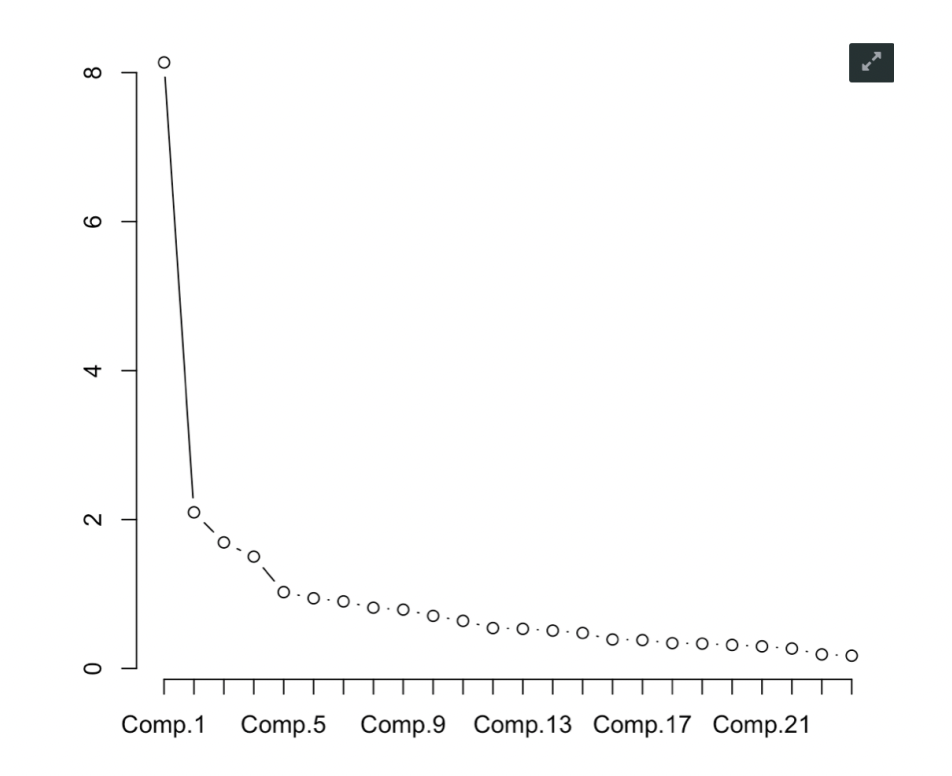
\includegraphics[scale=0.5]{elbow}
    \caption{}
    \label{}
\end{figure}\end{center}
第一个comp使第一个点到第二个点,...,第4个comp使第四个点到第五个点,所以这里我们只需要前4个comp.
\end{example}
2. Another way is to calculate the cumulative variance explained by the first PCs, and retain the number of $P C$ s explaining between $70 \%$ to $90 \%$ of the total variation.\\
3. An alternative way is to discard $\mathrm{PCs}$ such that $\lambda_{i}<\bar{\lambda}$


\subsection{Ridge Regression}
- Although the aim of PCR is to reduce dimensionality in the number of predictors, you still have to measure all the predictors since each $P C$ is a linear combination of all predictors.\\
- Ridge regression assumes that after normalization, some of the regression coefficients should not be very large.\\
- Ridge regression is very useful when you have collinearity and the LS regression coefficients are unstable.\\
- The method uses a \textbf{penalized regression} since the LS minimization problem has a penalty term:
$$
\operatorname{minimize}(y-X \boldsymbol{\beta})^{\top}(y-X \boldsymbol{\beta})+\lambda \sum_{j} \boldsymbol{\beta}_{j}^{2}
$$
for some $\lambda \geq 0$. The penalty term is $\sum_{j} \beta_{j}^{2}$\\
– Usually predictors are standardized first (centered by their means and scaled by their standard deviations) and the response $y$ is centered.\\
– The ridge regression estimates are:
$$\hat{\beta}=\left(\mathbf{X}^{T} \mathbf{X}+\lambda \mathbf{I}\right)^{-1} \mathbf{X}^{T} y$$
Or, the $\beta$ minimize
\begin{equation}
    \begin{aligned}
        (y-X\beta)^T(y-X\beta)\text{ subject to }\sum_{j} \boldsymbol{\beta}_{j}^{2}\leq t^2
    \end{aligned}
    \nonumber
\end{equation}
- The parameter $\lambda$ (or $t$) should be chosen to have stable estimates of $\beta$.\\

- Note that when $\lambda=0$ the ridge regression estimation problem reduces to the standard LS problem, while when $\lambda \rightarrow \infty, \hat{\boldsymbol{\beta}} \rightarrow 0$\\
- It is useful to plot the values of $\hat{\beta}_{j}$ as a function of $\lambda$.\\
- The value of $\lambda$ can be also chosen using automated methods as \textbf{Generalized Cross-Validation (GCV)} (similar to Cross-Validation).\\
- Ridge regression coefficient estimates are \textbf{biased}.

\subsection{Lasso Regression}
- In this case the estimated $\hat{\boldsymbol{\beta}}$ minimizes:
$$
\operatorname{minimize}(y-X \boldsymbol{\beta})^{\top}(y-X \boldsymbol{\beta})+\lambda \sum_{j}\left|\beta_{j}\right|
$$
for some $\lambda \geq 0$. The penalty term is $\sum_{j}\left|\beta_{j}\right|\left(L_{1}\right.$ constraint)\\
Or, the $\beta$ minimize
\begin{equation}
    \begin{aligned}
        (y-X\beta)^T(y-X\beta)\text{ subject to }\sum_{j}\left|\beta_{j}\right|\leq t
    \end{aligned}
    \nonumber
\end{equation}
- In two-dimensions the constraint defines a square. In higher dimensions it defines a polytope.\\
- Lasso is useful when the response can be explained by few predictors with zero effect on the remaining predictors (Lasso is similar to a variable selection method).\\
- When $\beta_{j}=0$ the corresponding predictor is eliminated. This is not the case for ridge regression.\\

- Use Lasso when the effect of predictors is \textbf{sparse}. This means that only few predictors will have an effect on the response (e.g. gene expression data) or when number of predictors is large $(p>n)$\\
- Use the lars $R$ package for Lasso\\
- Select $t$ in the constraint $\sum_{j=1}^{p}|\beta|_{j} \leq t$ by using \textbf{Cross-Validation (CV)}\\
- As $t$ increases, the number of predictors increases.

\subsection{Comparing Ridge Regression and Lasso}
\begin{center}\begin{figure}[htbp]
    \centering
    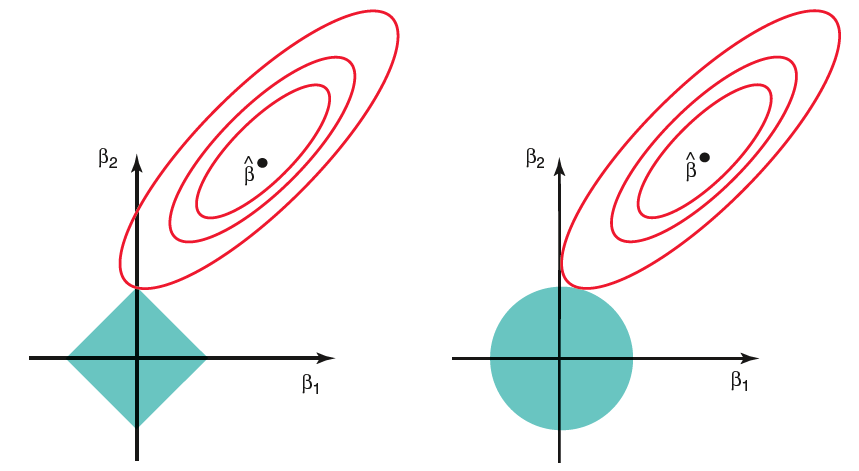
\includegraphics[scale=0.3]{compare.png}
    \caption{}
    \label{}
\end{figure}\end{center}
2维下,Lasso是正方形,Ridge是圆形。\\
- Lasso selects a sub-set of predictors (some coefficients equal to zero).\\
- Ridge regression performs better when the response is a function of many predictors with coefficients around the same size.\\
- Lasso will perform better when a relatively small number of predictors have large coefficients and the rest are very small or equal to zero.\\
- Since the number of predictors is never known a priori, cross-validation can be used to decide which approach is better for a particular data set.

\section{ANOVA: Comparative Experiments}
\subsection{Terminology}
- \textbf{Factor}: an Independent variable. They can be experimental or observational. In our example: Diet\\
- \textbf{Level}: A particular form of the factor. In our example: Levels of the Diet: $A, B, C, D$\\
- \textbf{Treatments}: Factor levels or factor level combinations (if the study contains more than one factors). They provide insights into mechanisms causing the variation being studied. Control treatments?\\
- \textbf{Complete Randomized Design}: Experimental units are randomly split into $r$ groups, and $r$ treatments are assigned, one per group.
\subsection{Data}
$$\begin{array}{ccccc}\text { group } 1 & y_{11}, & y_{12} & \ldots & y_{1 n_{1}} \\ \text { group } 2 & y_{21}, & y_{22} & \ldots & y_{2 n_{2}} \\ \vdots & \vdots & \vdots & \vdots & \vdots \\ \text { group } r & y_{r 1}, & y_{r 2} & \ldots & y_{r n_{r}}\end{array}$$
- $r$ is the number of groups\\
- $n_{i}$ denotes the number of obs in the ith group\\
- $n=\sum_{i=1}^{r} n_{i}$ is the total sample size\\
- $y_{i j}=$ observation $j$ for the ith factor.
\subsection{ANOVA Model}
\subsubsection{ANOVA Means Model (Cell Means Model)}
$$
y_{i j}=\mu_{i}+\varepsilon_{i j}, i=1, \ldots, r ; \quad j=1, \ldots, n_{i}
$$
- $y_{i j}$ : the value of the response in the $j$ th trial for the ith factor.\\
- $\mu_{i}$ : the population mean for the ith factor level (treatment).\\
- $\varepsilon_{i j} \sim^{i i d} \mathcal{N}\left(0, \sigma^{2}\right)$
\subsubsection{Factor Effects Model}
Define the effect of factor level $i$ on the response, i.e. the treatment effect as
$$
\alpha_{i}=\mu_{i}-\mu
$$
where $\mu$ is the overall mean.\\
Factor Effects Model:
$$
\begin{gathered}
y_{i j}=\mu+\alpha_{i}+\varepsilon_{i j}, i=1, \ldots, r ; j=1, \ldots, n_{i} \\
\varepsilon_{i j} \sim^{i i d} \mathcal{N}\left(0, \sigma^{2}\right)
\end{gathered}
$$
- The factor effects model has $r+1$ model parameters, i.e.
$$
\left(\mu, \alpha_{1}, \ldots, \alpha_{r}\right)
$$
- In order for the $\alpha$ 's to be (uniquely) estimated, we need to impose restrictions.\\
- The restrictions on the $\alpha$ 's depend on how $\mu$ is defined.
$$\begin{aligned}
    &\begin{array}{lcc}
    \hline \text { Model } & \mu \text { Definition } & \alpha \text { 's Restriction } \\
    \hline
    \text { Reference Cell } & \mu=\mu_{1} \quad \alpha_{1}=0 \\
    \text { Sum-to-Zero } & \mu=\frac{1}{r} \sum_{i} \mu_{i} & \sum_{i} \alpha_{i}=0 \\
    \text { Weighted Sum-to-Zero } & \mu=\frac{1}{n} \sum_{i} n_{i} \mu_{i} & \sum_{i} n_{i} \alpha_{i}=0 \\
    \hline
    \end{array}\\
    &\text { - The default in } \mathrm{R} \text { is the Reference Cell model. }
\end{aligned}
$$

\subsection{Model Properties}
$\begin{aligned}
&-E\left(y_{i j}\right)=\mu_{i} \\
&-\operatorname{Var}\left(y_{i j}\right)=\operatorname{Var}\left(\varepsilon_{i j}\right)=\sigma^{2}
\end{aligned}$\\
Thus, all observations have the same variance, regardless of factor level.\\
- $\varepsilon_{i j} \sim \mathcal{N}\left(0, \sigma^{2}\right)$ and independent\\
- $y_{i j} \sim \mathcal{N}\left(\mu_{i}, \sigma^{2}\right)$ and independent.\\
We can re-state the model as
\begin{center}
    $y_{i j}$ are independent $\mathcal{N}\left(\mu_{i}, \sigma^{2}\right)$
\end{center}
\subsection{Model Estimation}
Minimize the sum of squared deviations of the observations around their expected values with respect to the parameters:
$$
Q=\sum_{i=1}^{r} \sum_{j=1}^{n_{i}}\left(y_{i j}-\mathbb{E}\left(y_{i j}\right)\right)^{2}
$$
If we re-write $Q$ we have
$$
Q=\sum_{j}\left(y_{1 j}-\mu_{1}\right)^{2}+\sum_{j}\left(y_{2 j}-\mu_{2}\right)^{2}+\ldots+\sum_{j}\left(y_{r j}-\mu_{r}\right)^{2}
$$
So the \textbf{least squares estimator} of $\mu_{i}$, denoted by $\hat{\mu}_{i}$ is
$$
\hat{\mu}_{i}=\bar{y}_{i} .=\frac{1}{n_{i}} \sum_{j=1}^{n_{i}} y_{i j}
$$
Using the appropriate constraints, we can easily extract the estimators for $\mu$ and $\alpha_{i}$.\\
- The $L S$ fit for $y_{i j}$ is the corresponding group mean
$$
\hat{y}_{i j}=\bar{y}_{i}
$$
- Residuals
$$
r_{i j}=y_{i j}-\hat{y}_{i j}=y_{i j}-\bar{y}_{i}
$$
- RSS
$$
\sum_{i=1}^{r} \sum_{j=1}^{n_{i}}\left(y_{i j}-\bar{y}_{i} .\right)^{2}
$$
i.e. the within-group variation.

\begin{equation}
    \begin{array}{cccc}
    \hline
    \text { Source of Variation} & \text { SS } &\text { df } & \text { MS } \\
    \hline \hline \text { Between Groups}& F S S=\sum n_{i}\left(\bar{y}_{i.}-\bar{y}_{..}\right)^{2} & r-1 & \frac{F S S}{r-1} \\
    \text { Error (within Groups)}& R S S=\sum \sum\left(y_{i j}-\bar{y}_{i} .\right)^{2} & n-r & \frac{R S S}{n-r} \\
    \text { Total } & T S S=\sum \sum\left(y_{i j}-\bar{y}_{. .}\right)^{2} & n-1\\
    \hline \hline
    \end{array}
    \nonumber
\end{equation}

\subsection{F-test}
- We want to test whether the means of the groups are really different. We can express this as
$$
\left\{\begin{array}{l}
H_{0}: \mu_{1}=\mu_{2}=\ldots=\mu_{r} \\
H_{\alpha}: \text { not all } \mu_{i}, i=1, \ldots, r \text { are equal }
\end{array}\right.
$$
- or in terms of models
$$
\left\{\begin{array}{l}
H_{0}: y_{i j}=\mu+\varepsilon_{i j} \\
H_{\alpha}: y_{i j}=\mu+\alpha_{i}+\varepsilon_{i j}
\end{array}\right.
$$
- They are two nested models, so we can use the $F$-test
$$
\frac{\left(R S S_{0}-R S S_{\alpha}\right) /(r-1)}{R S S_{\alpha} /(n-r)} \sim F_{r-1, n-r}
$$
under $\mathrm{H}_{0}$.\\
- The test statistic can also be written as
$$
\frac{F S S /(r-1)}{R S S /(n-r)}=\frac{\text { Between-group Variation } /(r-1)}{\text { Within-group Variation } /(n-r)}
$$
where $F S S, R S S$ are defined in the ANOVA table.

\subsection{Diagnostics for ANOVA Models}
– Check for outliers/ unusual observations.\\
– Check the residuals vs. fitted values plot for departures from the constant variance assumption.\\
– Check the Q-Q plot for departures from the normality assumption.\\
\textbf{Levene’s Test} for Equality of Variances:\\
– Run Regression abs(residuals)∼ X, i.e. use abs(residuals) as the response in a new one-way ANOVA.\\
– If the p-value for the F-test is \textbf{greater} than 1\% level, then we conclude that there is no evidence of a non-constant variance.

\subsection{Inference for Factor Level Means (function about the $\mu_i$s)}
\subsubsection{A single factor level mean}
- Estimation of $$\mu_{i}: \hat{\mu}_{i}=\bar{y}_{i}$$
- Distribution of $$\hat{\mu}_{i}: E\left(\hat{\mu}_{i}\right)=\mu_{i}, \quad \operatorname{Var}\left(\hat{\mu}_{i}\right)=\frac{\sigma^{2}}{n_{i}}$$
- The estimated variance of $\bar{y}_{i}$. is $$s_{\bar{y}_{i}}^{2}=\frac{1}{n_{i}} \cdot \frac{R S S}{n-r}$$
- Under the ANOVA model assumptions
$\frac{\bar{y}_{i} \cdot-\mu_{i}}{s_{\bar{y}_{i}}}$ is distributed as $T_{n-r}$\\
- Confidence Interval for $\mu_{i}$ :
$$
\mu_{i} \in \bar{y}_{i} . \pm T_{n-r}(\alpha / 2) s_{\bar{y}_{i}}
$$


\subsubsection{A difference between two factor level means}
The difference between two factor level means (pairwise comparison) is defined as
$$
D=\mu_{i}-\mu_{i^{\prime}}
$$
- Estimation of $D$: $$\hat{D}=\bar{y}_{i}-\bar{y}_{i^{\prime}}$$
- Distribution of $\hat{D}$: $$E(\hat{D})=\mu_{i}-\mu_{i^{\prime}}, \operatorname{Var}(\hat{D})=\sigma^{2}\left(\frac{1}{n_{i}}+\frac{1}{n_{i^{\prime}}}\right)$$
The estimated variance of $\hat{D}$ is
$$
s_{\hat{D}}^{2}=\frac{R S S}{n-r} \cdot\left(\frac{1}{n_{i}}+\frac{1}{n_{i^{\prime}}}\right)
$$
- Under the ANOVA model assumptions
$$
\frac{\hat{D}-D}{s_{\hat{D}}} \text { is distributed as } T_{n-r}
$$
- Confidence Interval for $D$: $$D \in \hat{D}\pm T_{n-r}(\alpha / 2) s_{\hat{D}}$$
- Hypothesis Test for $D:$
$$
\left\{\begin{array} { l } 
{ H _ { 0 } : \mu _ { i } = \mu _ { i ^ { \prime } } } \\
{ H _ { \alpha } : \mu _ { i } \neq \mu _ { i ^ { \prime } } }
\end{array} \Leftrightarrow \left\{\begin{array}{l}
H_{0}: \mu_{i}-\mu_{i^{\prime}}=D=0 \\
H_{\alpha}: \mu_{i}-\mu_{i^{\prime}} \neq 0
\end{array}\right.\right.
$$
The test statistic is $$t=\frac{\hat{D}}{s_{\hat{D}}} \sim T_{n-r}$$





\subsubsection{A contrast among factor level means}
A contrast is a comparison involving two or more level means:
$$
L=\sum_{i=1}^{r} c_{i} \mu_{i}, \quad \text { where } \sum_{i=1}^{r} c_{i}=0
$$
- Estimation of $L$: $$\hat{L}=\sum_{i=1}^{r} c_{i} \bar{y}_{i}$$
- Distribution of $\hat{L}$: $$E(\hat{L})=\sum_{i=1}^{r} c_{i} \mu_{i}, \operatorname{Var}(\hat{L})=\sigma^{2} \sum_{i=1}^{r} \frac{c_{i}^{2}}{n_{i}}$$
The estimated variance of $\hat{L}$ is
$$
s_{\hat{L}}^{2}=\frac{R S S}{n-r} \cdot \sum_{i=1}^{r} \frac{c_{i}^{2}}{n_{i}}
$$
- Under the ANOVA model assumptions
$\frac{\hat{L}-L}{s_{\hat{L}}}$ is distributed as $T_{n-r}$\\
- Confidence Interval for $L$: $$L \in \hat{L}\pm T_{n-r}(\alpha / 2) s_{\hat{L}}$$
- Hypothesis Testing for $L:$
$$
\left\{\begin{array}{l}
H_{0}: L=0 \\
H_{\alpha}: L \neq 0
\end{array}\right.
$$
The test statistic is $$t=\frac{\hat{L}}{s_{\hat{L}}} \sim T_{n-r}$$


\subsubsection{A linear combination of factor level means}
$$
L=\sum_{i=1}^{r} c_{i} \mu_{i}, \quad \text { no restrictions on } c_{i}^{\prime} s
$$
- Point estimator and estimated variance same as before.\\
- Single Degree of Freedom Tests
$$
\left\{\begin{array}{l}
H_{0}: L=c \\
H_{\alpha}: L \neq c
\end{array}\right.
$$
The test statistic here is
$$
F=t^{2}=\left(\frac{\hat{L}-c}{s_{\hat{L}}}\right)^{2} \sim F_{1, n-r}
$$
\subsection{Limitations of Inference Procedures}
The confidence coefficient $1-\alpha$ for the estimation procedures described is a statement confidence coefficient and applies \textbf{only to a particular estimate}, \textbf{not to a series of estimates}.\\
Similarly the specified Type I error rate $\alpha$ applies only to a particular test and not to a series of tests.

\subsection{Bonferroni Correction $\frac{\alpha}{m}$}
\begin{example}
If the confidence coefficents are $95\%$ for all individual $\mu_i$, the confidence coefficient will be $(95\%)^n<95\%$ for family $f(\mu_1,...,\mu_n)$.\\
So the $95\%$ confidence interval of family will be \textbf{wider} than individual.
\end{example}


When? The family of interest is a particular set of pairwise comparisons, contrasts, or linear combinations that is specified by the user.\\
- Suppose $m$ is the number of statements in the family.\\
- In order to control the family wise error rate to be $\alpha$, we need to reduce the error rate for each individual comparison to be $\alpha / m$.\\
- That is we need to increase the significance level from $(1-\alpha)$ to $(1-\alpha / m)$\\
- Not applicable when $m$ is large, since the Cls would be too wide due to the increase of the significant level.

i.e. 我们用 $1-\frac{5\%}{n}$ for all $\mu_i$ 组成 $95\%$的$f(\mu_1,...,\mu_n)$


\subsection{Tukey’s Paired Comparison Procedures}
When? the family of interest is a set of all pairwise comparisons of factor level means, i.e. it consists of estimates of all pairs $D=\mu_{i}-\mu_{i^{\prime}}$\\
A confidence interval is given by
$$
D \in \hat{D}+\frac{q(\alpha / 2 ; r, n-r)}{\sqrt{2}} s(\hat{D})
$$
where $q(\alpha / 2 ; r, n-r)$ refers to the $\alpha / 2$ upper quantile of the studentized range for $r$ means and $n-r$ degrees of freedom.\\
The coverage probability is exact when the sample sizes in each group are identical and is approximate otherwise.\\
Remark: The studentized range refers to the distribution of
$$
\max _{i \neq j} \sqrt{n}\left(\bar{y}_{i}-\bar{y}_{j}\right) / \hat{\sigma}
$$
where $\bar{y}_{i}$ and $\bar{y}_{j}$ are sample means from independent samples of size $n$ from normal distributions with common means and variance $\sigma^{2}$.\\
\textbf{Note}: Tukey is always better than Bonferroni and Scheffe in pairwise comparisons.

\subsection{Scheffe’s Method for Contrasts}
When? The family of interest is the set of contrasts among the factor level means:
$$
L=\sum c_{i} \mu_{i}, \text { where } \sum c_{i}=0
$$
An confidence interval is given by
$$
L \in \hat{L}+(r-1) F_{r-1, n-r}(\alpha) s_{\hat{L}}
$$


\section{Two Way ANOVA}
Single-factor:\\
1. Do not explore the entire space of treatment combinations.

2. Interactions cannot be estimated.

3. Full randomization is not possible.

4. Multiple stages increase complexity of the analysis.

MultiFactor:\\
1. Efficient replication.

2. Assessment of Interactions.

3. Validity of Findings.

\subsection{Factor Effects Model for Two Factors}
$$y_{ijk}=\mu+\alpha_i+\beta_j+(\alpha\beta)_{ij}+\varepsilon_{ijk}$$
\begin{equation}
    \begin{array}{lll}
    \hline & \text { Sum } & \text { Average } \\
    \hline \hline \text { Cell }(i, j) & y_{i j .}=\sum_{k=1}^{n} y_{i j k} & \bar{y}_{i j .}=\frac{y_{i j}}{n} \\
    \text { Row } i & y_{i . .}=\sum_{j=1}^{b} \sum_{k=1}^{n} y_{i j k} & \bar{y}_{i . .}=\frac{y_{i . .}}{b n} \\
    \text { Column } j & y_{j . j}=\sum_{i=1}^{a} \sum_{k=1}^{n} y_{i j k} & \bar{y}_{j .}=\frac{y_{j . j}}{a n} \\
    \text { Overall } & y_{...}=\sum_{i=1}^{a} \sum_{j=1}^{b} \sum_{k=1}^{n} y_{i j k} & \bar{y}_{...}=\frac{y_{...}}{n a b} \\
    \hline
    \end{array}
    \nonumber
\end{equation}
- Using least squares method, the estimated treatment means are:
$$
\hat{\mu}_{i j}=\bar{y}_{i j}
$$
- The factor effects estimators depend on the constraints that we impose. For example, under the sum-constraints we have
$$
\begin{gathered}
\hat{\alpha}_{i}=\bar{y}_{i . .}-\bar{y} \ldots, \quad \hat{\beta}_{j}=\bar{y}_{. j .}-\bar{y} \ldots \\
(\hat{\alpha \beta})_{i j}=\bar{y}_{i j}-\bar{y}_{i .}-\bar{y}_{. j}+\bar{y} . .
\end{gathered}
$$
- The fitted values and residuals compute as usual as
$$
\hat{y}_{i j k}=\bar{y}_{i j}, \quad r_{i j}=y_{i j k}-\hat{y}_{i j k}
$$

\subsection{Interaction Plots}
\begin{center}\begin{figure}[htbp]
    \centering
    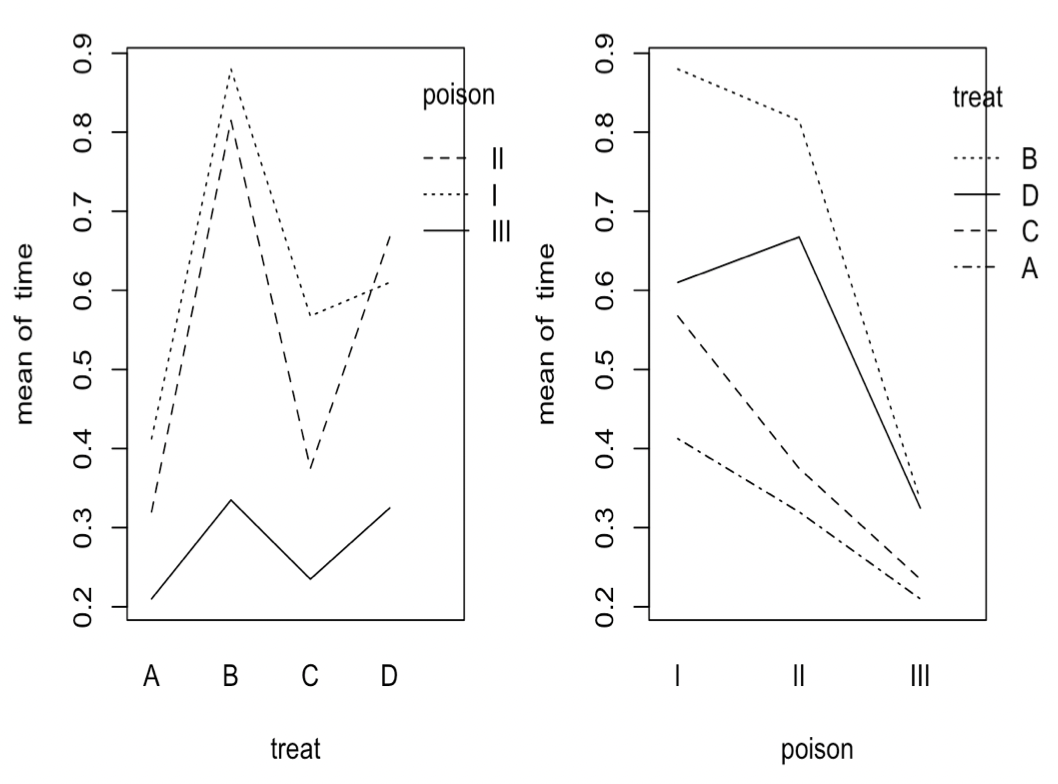
\includegraphics[scale=0.5]{IP}
    \caption{}
    \label{}
\end{figure}\end{center}
If the lines are not parallel, interaction is presented.

\subsection{Partitioning of Total Sum of Squares}
$$\begin{aligned} \underbrace{y_{i j k}-\bar{y}_{...}}_{\text {Total Deviation }}=& \underbrace{\bar{y}_{i j}-\bar{y} _{...}}_{\begin{array}{c}\text { Deviation of estimated } \\ \text { treatment mean around } \\ \text { overall mean }\end{array}}+\underbrace{y_{i j k}-\bar{y}_{i j.}}_{\begin{array}{c}\text { Deviation } \\ \text { around estimated } \\ \text { treatment mean }\end{array}} \\ & T S S=F S S+R S S \end{aligned}$$
where
$$
\begin{aligned}
&T S S=\sum_{i} \sum_{j} \sum_{k}\left(y_{i j k}-\bar{y} _{...}\right)^{2} \\
&F S S=n \sum_{i} \sum_{j}\left(\bar{y}_{i j \cdot}-\bar{y} _{...}\right)^{2} \\
&R S S=\sum_{i} \sum_{j} \sum_{k}\left(y_{i j k}-\bar{y}_{i j.}\right)^{2}=\sum_{i} \sum_{j} \sum_{k} e_{i j k}^{2}
\end{aligned}
$$

\subsection{Partitioning of Treatment Sum of Squares}
$$\underbrace{\bar{y}_{i j.}-\bar{y}_{...}}_{\begin{array}{c}\text { Deviation of estimated } \\ \text { treatment mean around } \\ \text { overall mean }\end{array}}=\underbrace{\bar{y}_{i . .}-\bar{y}_{...}}_{\begin{array}{c}\text { A main } \\ \text { effect }\end{array}}+\underbrace{\bar{y} _{.j.}-\bar{y}_{...}}_{\begin{array}{c}\text { B main } \\ \text { effect }\end{array}}+\underbrace{\bar{y}_{i j.}-\bar{y}_{i . .}-\bar{y} _{.j.}+\bar{y} _{...}}_{\begin{array}{c}\text { A B interaction } \\ \text { effect }\end{array}}$$
$$
F S S=S S A+S S B+S S A B \text { (Orthogonal Decomposition) }
$$
where
$$
\begin{aligned}
S S A &=n b \sum_{i}\left(\bar{y}_{i . .}-\bar{y} \ldots\right)^{2} \\
S S B &=n a \sum_{j}\left(\bar{y}_{. j .}-\bar{y} \ldots\right)^{2} \\
S S A B &=n \sum_{i} \sum_{j}\left(\bar{y}_{i j .}-\bar{y}_{i . .}-\bar{y}_{. j .}+\bar{y} \ldots\right)^{2}
\end{aligned}
$$

\subsection{ANOVA Table}
\begin{equation}
    \begin{array}{cccc}
    \hline \text { Source of Variation } & \text { SS } & \text { df } & \text { MS } \\
    \hline \hline \text { Factor A } & \text { SSA } & a-1 & \text { MSA }=\frac{S S A}{a-1} \\
    \text { Factor B } & \text { SSB } & b-1 & \text { MSB }=\frac{S S B}{b-1} \\
    \text { AB Interactions } & \text { SSAB } & (a-1)(b-1) & \text { MSAB }=\frac{S S A B}{(a-1)(b-1)} \\
    \text { Error } & \text { RSS } & a b(n-1) & \text { MSE }=\frac{R S S}{a b(n-1)} \\
    \text { Total } & \text { TSS } & \text { nab }-1 & \\
    \hline
    \end{array}
    \nonumber
\end{equation}

\subsection{F-test}
- In order to test for the statistical significance of the interaction terms, we use partial $F$-tests. So, we fit a main effects model (i.e. no interactions)
$$
y_{i j k}=\mu+\alpha_{i}+\beta_{j}+e_{i j k}
$$
- Then, we compare the two nested models:
$$
\left\{\begin{array}{l}
H_{0}: \text { smaller model with } p_{0} \text { coefficients } \\
H_{\alpha}: \text { larger model with } p_{\alpha} \text { coefficients }
\end{array}\right.
$$
The $F$-test is formulated as
$$
F=\frac{\left(R S S_{0}-R S S_{\alpha}\right) /\left(p_{\alpha}-p_{0}\right)}{M S E_{\alpha}} \sim F_{p_{\alpha}-p_{0}, n-p_{\alpha}} \text { under the } H_{0}
$$
We can also perform F-tests directly using the ANOVA table, where for the interaction term we have:
$$F_{AB}=\frac{MSAB}{MSE}\sim F_{(a-1)(b-1),nab-1}$$
Hierarchy principle: we test for main effects only if the interaction term is not statistically significant.

\subsection{Estimation of Factor Level Means}
When interactions are not statistically significant, we analyze the factor level means:\\
- Factor Level Means: $$\hat{\mu}_{i.}=\bar{y}_{i. .}, s_{\hat{\mu}_{i} .}^{2}=\frac{M S E}{b n}$$
- Differences of Factor Level Means:
$$
\hat{\mu}_{i \cdot}-\hat{\mu}_{i^{\prime} .}=\bar{y}_{i . .}-\bar{y}_{i^{\prime} . .,}, s_{\hat{D}}^{2}=\frac{2 M S E}{b n}
$$
- Contrasts of Factor Level Means:
$$
\hat{L}=\sum c_{i} \hat{\mu}_{i .}=\sum c_{i} \bar{y}_{i . . .}, s_{\hat{L}_{(i)}}^{2}=\frac{M S E}{b n} \sum c_{i}^{2}
$$
where $\sum c_{i}=0$

For individual hypothesis test and $\mathrm{Cls}$, the multiplier is $T_{(n-1) a b}(\alpha / 2)$.\\
For family hypothesis tests/intervals, we select the desired family multiplier:\\
- Tukey Multiplier: $$\frac{1}{\sqrt{2}} q_{a,(n-1) a b}(1-\alpha)$$
- Bonferroni Multiplier: $B=T_{(n-1) a b}(1-\alpha / 2 m)$, where $m$ refers to the number of multiple comparisons.\\
- Scheffé Multiplier:\\
- $S^{2}=(b-1) F_{b-1,(n-1) a b}(1-\alpha)$, if the contrasts involve the $\mu_{i}$. and\\
- $S^{2}=(a-1) F_{a-1,(n-1) a b}(1-\alpha)$, if the contrasts involve the $\mu . j$.



\subsection{Estimation of Treatment Means}
When interactions are statistically significant, we analyze the treatment means:\\
- Treatment Means: $$\hat{\mu}_{i j}=\bar{y}_{i j.}, \quad s_{\hat{\mu}_{i j}}^{2}=\frac{M S E}{n}$$
- Differences of Treatment Means:
$$
\hat{D}=\hat{\mu}_{i j}-\hat{\mu}_{i^{\prime} j^{\prime}}=\bar{y}_{i j.}-\bar{y}_{i^{\prime} j^{\prime} .}, \quad i, j \neq i^{\prime}, j^{\prime} \text { and } s_{\hat{D}}^{2}=\frac{2 M S E}{n}
$$
- Contrasts of Treatment Means:
$$
\hat{L}=\sum \sum c_{i j} \hat{\mu}_{i j}=\sum \sum c_{i j} \bar{y}_{i j}, \text { where } \sum \sum c_{i j}=0
$$
with variance $s_{\hat{L}}^{2}=\frac{M S E}{n} \sum c_{i j}^{2}$\\
For individual hypothesis test and Cls, the multiplier is $T_{(n-1) a b}(\alpha / 2)$.\\
For family hypothesis tests/intervals, we choose the desired family multiplier:\\
- Tukey Multiplier: $\frac{1}{\sqrt{2}} q_{a b,(n-1) a b}(1-\alpha)$\\
- Bonferroni Multiplier: $B=T_{(n-1) a b}(1-\alpha / 2 m)$, where $m$ refers to the number of multiple comparisons.\\
- Scheffé Multiplier: $S^{2}=(a b-1) F_{a b-1,(n-1) a b}(1-\alpha)$, if the contrasts involve the $\mu_{i . .}$



\section{Two Way ANOVA: Special Cases}
\subsection{Unbalanced ANOVA (Use \textbf{Partial $F-$Test} or ANOVA type III in R)}
–\ \textbf{When the treatment sample sizes are unequal}, the analysis of variance for two-factor studies becomes more complex.

–\ The least-squares equations are no longer of a simple structure and the regular analysis of variance formulas are now inappropriate.

–\ Furthermore, the factor effect component sum of squares are no longer orthogonal; that is, they \textbf{do not sum up to TSS}.

$$y_{ijk}=\mu+\alpha_i+\beta_j+(\alpha\beta)_{ij}+\varepsilon_{ijk}$$

–\ Due to the lack of orthogonality, the \textbf{ANOVA F-tests are not applicable}.

\subsubsection{ Use \textbf{Partial $F-$Test}}
–\ We will express the ANOVA model as a regression model with \textbf{indicator (dummy) variables}.

–\ We need $a − 1$ indicator variables for factor $A$ main effects and $b − 1$ indicator variables for factor $B$ main effects. The interactions correspond to the cross products of the indicator variables for A and B.

Use \textbf{Partial $F-$Test}.

\subsubsection{ANOVA type III in R}
This type tests for the presence of an effect given that both the other effects are in the model.
\begin{center}\begin{figure}[htbp]
    \centering
    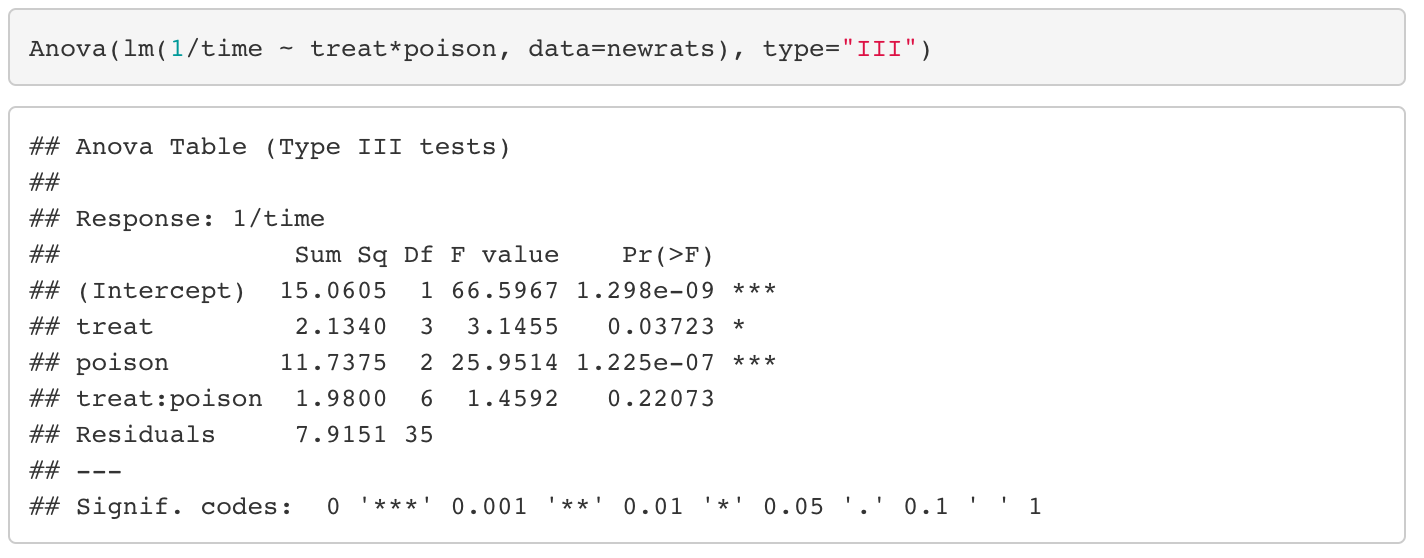
\includegraphics[scale=0.3]{type3}
    \caption{}
    \label{}
\end{figure}\end{center}
\begin{example}
Compute SSTotal
\end{example}
\begin{equation}
    \begin{aligned}
        {RSS}_0-{RSS}_\alpha=&(SSA+SSR)-SSR&=SSA&=2.1340\\
        &(SSB+SSR)-SSR&=SSB&=11.7375\\
        &(SSAB+SSR)-SSR&=SSAB&=1.9800\\
        &	&SST&=2.1340+11.7375+1.9800+7.9151=23.7666
    \end{aligned}
    \nonumber
\end{equation}







\subsection{ Balanced ANOVA with $n = 1$ (Tukey’s Test)}
-\ Only one observation in each cell, so we cannot fit the interaction model.

-\ There are no degrees of freedom left for estimating the error.

-\ RSS = 0 when the model includes main effects and interaction term. (error is 0)

-\ All F-tests are valid, but the interaction model is not a candidate model.

\subsubsection{ Tukey’s Test for Additivity}
Consider the following model that includes interactions:
$$y_{ij}=\mu+\alpha_i+\beta_j+\theta\alpha_i\beta_j+\varepsilon_{ij}$$

Here, we assume that the interactions are of \textit{multiplicative} nature, i.e.
$$(\alpha\beta)_{ij}=\theta\alpha_i\beta_j$$

-\ Consider the SSA, SSB as before and:
$$
{S S A B}^{*}=\frac{\left(\sum_{i} \sum_{j}\left(\bar{y}_{i}-\bar{y}_{. .}\right)\left(\bar{y}_{. j}-\bar{y} . .\right) y_{i j}\right)^{2}}{\sum_{i}\left(\bar{y}_{i .}-\bar{y} . .\right)^{2} \sum_{j}\left(\bar{y}_{. j}-\bar{y} . .\right)^{2}}
$$
- The TSS is computed as usual and is decomposed as
$$
T S S=S S A+S S B+{S S A B}^{*}+{S S R e m}^{*}
$$
where the remainder is
$$
{S S R e m}^{*}=T S S-S S A-S S B-S S A B^{*}
$$

- We want to test the following hypothesis
$$
\begin{cases}H_{0}: \theta=0 & \text { (no interactions) } \\ H_{\alpha}: \theta \neq 0 & \text { (interactions) }\end{cases}
$$
which is essentially a test for model additivity.
- The test statistic computes as
$$
F^{*}=\frac{{S S A B}^{*} / 1}{{S S R e m}^{*} /(a b-a-b)}
$$


\section{Introduction to Experimental Designs}
\subsection{ Experimental vs. Observational Study}
\textit{Experimental Study} is a scienti c procedure undertaken to make a discovery, test a hypothesis or verify a claim.\\
\textit{Observational Study} is one in which the experimenter observes the effect of a factor on the response, or measures an outcome without an attempt to a ect the outcome by intervention.

\subsection{ Principles of Experimental Design}
Randomization\\
- Random allocation of treatment and order\\
- Ensures that collected data are IID random variables\\
- Averages-out the effects of exogenous factors.\\

Replication\\
- Estimate of experimental error\\
- Higher Precision\\

Blocking\\
- Higher precision when comparisons of factors are made\\
- Reduced variability transmitted from nuisance factors.\\


\subsection{ Randomization Test}
- A test based directly on re-randomizing - with the same kind of randomization originally used to assign the treatments - is called a \textbf{randomization test}.\\

- \textit{Advantage}: No need for any distributional assumptions (independence, normality, etc.) - just need to assume that the treatment randomization was performed properly.\\
- \textit{Disadvantage}: Requires more computation, and you must implement for yourself or use specialized software.

\section{ Blocking in Experimental Designs}

\subsection{ Randomized Complete Block Design (RCBD) Model}
Example:\\
\begin{center}\begin{figure}[htbp]
    \centering
    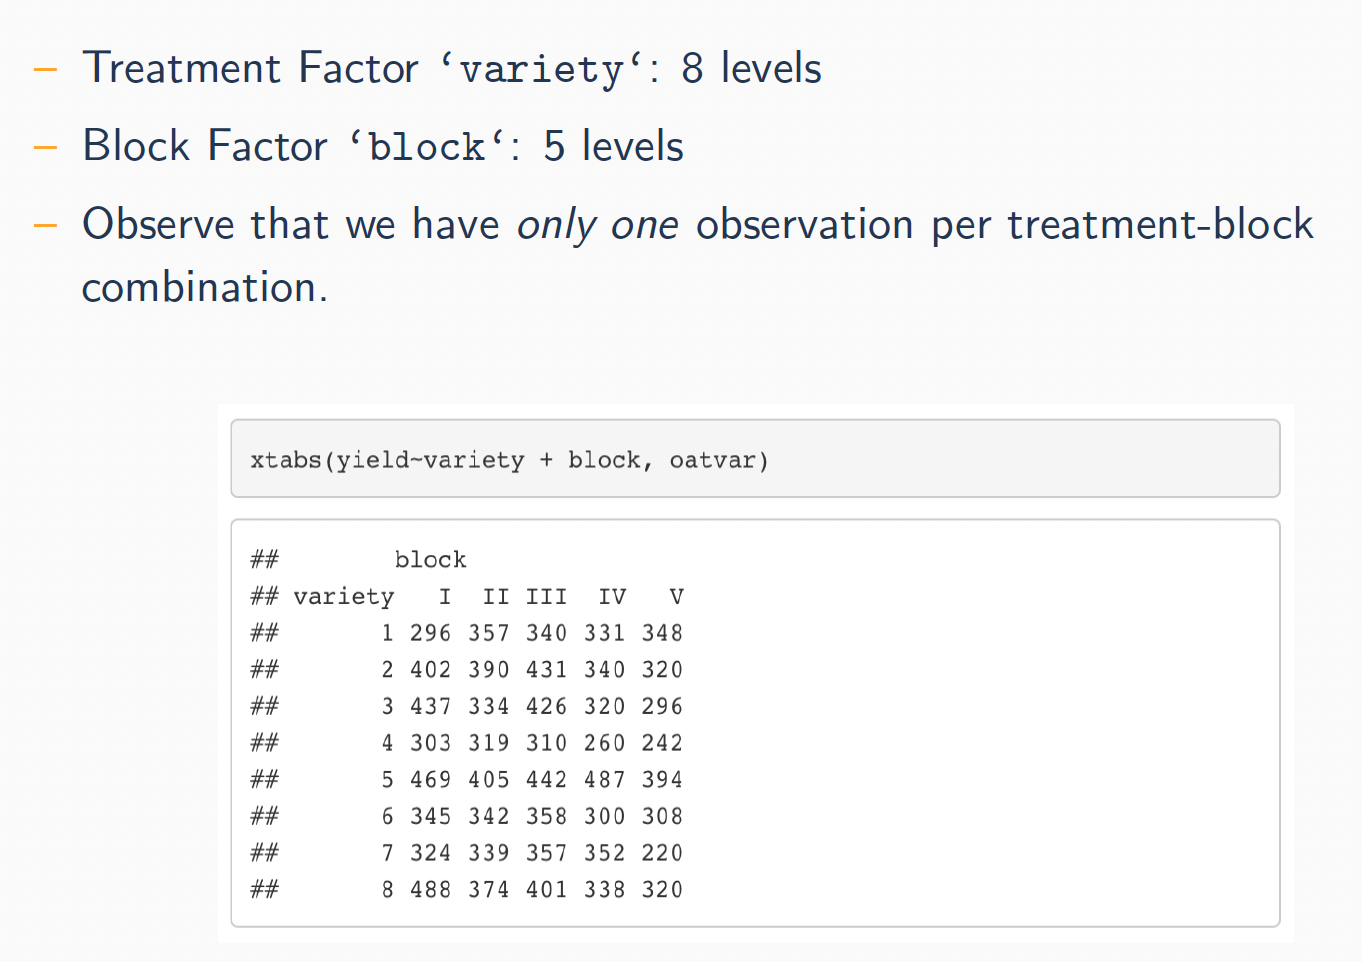
\includegraphics[scale=0.5]{CRBD_example.png}
    \caption{}
    \label{}
\end{figure}\end{center}

Suppose that there are $r$ treatments (factor levels) and $n_b$ blocks.
$$
y_{i j}=\mu+\tau_{i}+\beta_{j}+\varepsilon_{i j}
$$
where\\
- $\mu .$ is a constant\\
- $\tau_{i}$ are the treatment effects\\
- $\beta_{j}$ are the block effects\\
- $\varepsilon_{i j}$ are independent $\mathcal{N}\left(0, \sigma^{2}\right)$\\
- $i=1, \ldots, n_{b}$ (total number of blocks), $j=1, \ldots, r$ (total number of treatments)\\

Remarks\\
- $y_{i j}$ is the response for the $j$ th treatment in the ith block.\\
- There is a single observation per block. This implies that we have a limited ability to detect an interaction between treatment and block. So, we are working with the additive model.\\
- We can check for treatment and block main effects, but blocking is a feature of the design which means that if insignificant, we cannot gain the degrees of freedom.\\

ANOVA Display for the RCBD (Two factors: Treatments and Blocks)\\
\begin{tabular}{|l|l|l|l|c|}
\hline Source of Variation & Sum of Squares & Degrees of Freedom & Mean Square & $F_{0}$ \\
\hline Treatments & $S S_{\text {Treatments }}$ & $r-1$ & $\frac{S S_{\text {Treatments }}}{r-1}$ & $\frac{M S_{\text {Treatments }}}{M S_{g}}$ \\
\hline Blocks & $S S_{\text {Blocks }}$ & $n_b-1$ & $\frac{S S_{\text {Blocks }}}{n_b-1}$ & \\
\hline Error & $S S_{E}$ & $(r-1)(n_b-1)$ & $\frac{S S_{g}}{(r-1)(n_b-1)}$ & \\
\hline Total & $S S_{T}$ & $rn_b-1$ & & \\
\hline
\end{tabular}





\subsection{ Latin Squares}

\subsubsection{Example}
- A, B, C: 3 treatments\\
- Day of week (Monday, Wednesday, Friday): Blocking Variable\\
- Operator ID: 1, 2, 3: Blocking Variable\\
\begin{center}
\begin{tabular}{cccc}
& \multicolumn{3}{c}{ Operator } \\
Day & 1 & 2 & 3 \\
\hline Monday & $B$ & $A$ & $C$ \\
Wednesday & $A$ & $C$ & $B$ \\
Friday & $C$ & $B$ & $A$ \\
\hline
\end{tabular}
\end{center}
* Each operator runs each treatment, and all treatments are run on each day


\subsubsection{ Features of a Latin Square Design}
- There are $r$ treatments.\\
- There are 2 blocking variables, each containing $r$ classes.\\
- Each row and each column in the design square contains all treatments.\\
- Each treatment is assigned to each block only once.\\

Advantages\\
- Reduces more experimental error than with 1 blocking factor.\\
- Small scale studies can isolate important treatment features.\\
- Repeated measures designs can remove order effects.\\

Disadvantages\\
- Each blocking factor must have $r$ levels.\\
- No interactions among factors.\\
- With small $r$, we have very few error degrees of freedom.\\
- Complex Randomization.\\

\subsubsection{ Randomization in Latin Square Designs}
- Determine $r$, the number of treatments, row blocks, and column blocks.\\
- Select a Standard Latin Square (from tables or with software).\\
- Use Capital Letters to represent treatments $(A, B, C, \ldots)$ and randomly assign treatments to labels.\\
- Randomly assign Row Block levels to Square Rows.\\
- Randomly assign Column Block levels to Square Columns.\\

\subsubsection{ Latin Square Model}
$$
y_{i j k}=\mu+\tau_{i}+\beta_{j}+\gamma_{k}+e_{i j k}
$$
where\\
- $\mu$ is a constant\\
- $\tau_{i}$ treatment effect (latin letter)\\
- $\beta_{j}$ (column) blocking effect\\
- $\gamma_{k}$ (row) blocking effect\\
- $e_{i j k}$ are independent $\mathcal{N}\left(0, \sigma^{2}\right)$\\
- $i, k, j=1, \ldots, r$\\

NOVA Display for the Latin Square Model (Three factors: Treatments, Rows and Cols)
$$\begin{array}{lcc}\text { AOV } & d f  \\ \text { Rows (blocks)} & r-1  \\ \text { Cols (blocks)} & r-1  \\ \text { Treatments } & r-1  \\ \text { Error } & (r-1)(r-2)  \\ \text { Total } & \left(r^{2}-1\right)\end{array}$$












\subsection{ Balanced Incomplete Block Design (BIBD)}

- $[\rightarrow]$ Why Balanced?\\
Each pair of treatments occur together $\lambda$ times.\\
- $[\rightarrow]$ Why Incomplete?\\
Cannot fit all treatments in each block.\\

Notation\\
- $t$ treatments\\
- $b$ blocks\\
- $k$ treatments per block (block size)\\
- $r$ times each treatment occurs\\
- $N=t \cdot r=b \cdot k$ observations in total\\

- Treatment $i$ occurs in $r$ blocks.\\
- To have balance, each other treatment is equally likely to be treatment $i$ in a block.\\
- Since there are $k-1$ other units in a block and $t-1$ other treatments, the number of times each pair of treatments appears in the same block is
\begin{equation}
    \begin{aligned}
        \lambda&=\text{一个block中剩余的units可能存在treatment j 的概率}\times \text{treatment i 总共存在的block数量}\\&=\frac{k-1}{t-1}r=\frac{r(k-1)}{t-1}
    \end{aligned}
    \nonumber
\end{equation}
where $\lambda$ is an integer.\\

Examples\\
- $t=3, b=3, k=2 \rightarrow r=2, \lambda=1$.\\
$t=$\# treatments $\{A,B,C\}=3$\\
The form of square: $k\times b=2\times 3$.\\
$r=$\# A occurs=\# B occurs=\# C occurs$=2$\\
$\lambda=$\# A and B in one block=\# A and C in one block=\# B and C in one block$=1$
\begin{center}
    Block\\
\begin{tabular}{|c|c|c|}
\hline 1 & 2 & 3 \\
\hline A & B & A \\
\hline B & C & C \\
\hline
\end{tabular}
\end{center}

- $t=4, k=2, b=6 \rightarrow r=3, \lambda=1$
\begin{center}
Block\\
\begin{tabular}{|c|c|c|c|c|c|}
\hline 1 & 2 & 3 &4 &5&6 \\
\hline A & A & A& B & B & C \\
\hline B& C & D & C & D & D \\
\hline
\end{tabular}
\end{center}


\subsection{ BIBD Remarks}
Advantages:\\
- A BIBD enables us to run an experiment when the size of the available blocks of experimental units is smaller than the number of treatments.\\
- Estimates of treatment effects have equal precision and expressions for the variances of the estimated cell means and of contrasts of treatment means or effects are relatively simple.\\
- The presence of balance permits the use of Scheffé and Tukey procedures for the analysis of treatment effects.\\

Disadvantages:\\
- BIBD exist only for certain combinations of numbers of treatments, block sizes, and numbers of blocks.\\
- The assumption that there are no interactions between the blocking variable and the treatments is restrictive.\\
- The analysis of a BIBD is more complex than that of a RCBD.\\

$$
y_{i j}=\mu+\tau_{i}+\beta_{j}+e_{i j}
$$
- $\mu$ constant\\
- $\tau_{i}$ treatment effects\\
- $\beta_{j}$ the block effects\\
- $e_{i j}$ independent $N\left(0, \sigma^{2}\right)$\\

Remarks\\
- Not all $y_{i j}$ exist, because of incompleteness.\\
- Non-orthogonality of treatments and blocks.\\





\section{ Linear Models with Random Effects}
\subsection{ Random Effects}
One-way ANOVA model
$$
y_{i j}=\mu+\alpha_{i}+\varepsilon_{i j}
$$
Previously, we assumed the $\alpha_{i}$ s were parameters: fixed, unknown values. (We also gave a restriction, to make them identifiable.) These are fixed effects, corresponding to a fixed factor.\\
Now suppose that the $\alpha_{i}$ s are unobserved random variables:
$$
\alpha_{i} \sim N\left(0, \sigma_{\alpha}^{2}\right)
$$
and assume they are independent of each other and of the $\varepsilon_{i j}$ s.\\
These $\alpha_{i}$ s are called random effects, and the corresponding factor variable is a random factor.\\

- \textbf{Fixed effects} are appropriate when the levels of the factor are individually important or meaningful (e.g. treatments in a designed experiment, levels of education).\\
- \textbf{Random effects} are appropriate when the levels of the factor are meaningful only as representatives of a more general collection (e.g. as if sampled from a population, or representative of some hypothetical population).\\

- For the one-way ANOVA model with a random factor, the random effects satisfy
$$
\mathrm{E}\left(\alpha_{i}\right)=0 \quad \operatorname{Var}\left(\alpha_{i}\right)=\sigma_{\alpha}^{2}
$$
so \underline{random effects contribute only to the variance structure of the model}, not to the mean structure.\\
- The parameter $\sigma_{\alpha}^{2}$ is generally unknown, and we usually seek to estimate it $\left(\right.$ or $\left.\sigma_{\alpha}\right)$ and test the null hypothesis $\sigma_{\alpha}^{2}=0 .$\\
Parameters like $\sigma_{\alpha}^{2}$ (and $\sigma^{2}$) are called \textbf{variance components}.\\

\subsection{ Intraclass Correlation}
- Under this model, the responses can be correlated:
$$
\operatorname{Cov}\left(y_{i j}, y_{i j^{\prime}}\right)=\sigma_{\alpha}^{2} \quad \text { for } j \neq j^{\prime}
$$
So different observations from the same "class" (same level $i$ of the random factor) may have a nonzero correlation.\\
- The \textbf{intraclass correlation coefficient (ICC)} is the correlation between $y_{i j}$ and $y_{i j^{\prime}}$ (for any $i$ and $j \neq j^{\prime}$ ):
$$
\rho=\frac{\sigma_{\alpha}^{2}}{\sigma_{\alpha}^{2}+\sigma^{2}}
$$

\subsection{ Mixed Models}
- A \textbf{fixed effects model} has only fixed factors.\\
- A \textbf{random effects model} has only random factors.\\
- A \textbf{mixed (effects) model} has both fixed and random factors.\\
The general form (matrix-vector):
$$
\mathrm{y}=\mathrm{X} \beta+\mathrm{Z}_{\gamma}+\varepsilon
$$
where $\mathbf{X}$ and $\mathbf{Z}$ are known design matrices, $\beta$ contains the fixed effect (mean-related) parameters, and
$$
\gamma \sim N\left(0, \sigma^{2} D\right) \quad \text { independent of } \quad \varepsilon \sim N\left(0, \sigma^{2} I\right)
$$
are the random effects and the errors, with D containing the (unknown) random effect parameters.\\

The variance components (in D) are typically estimated via one of three different methods:\\
- \textbf{ANOVA estimation}, based on quantities in an ANOVA table; complicated for general models\\
- \textbf{maximum likelihood}\\
- \textbf{restricted maximum likelihood (REML)}, generally less biased than maximum likelihood\\
For balanced data, REML and ANOVA estimation tend to coincide.

\subsection{REML: restricted maximum likelihood}
\begin{center}\begin{figure}[htb]
    \centering
    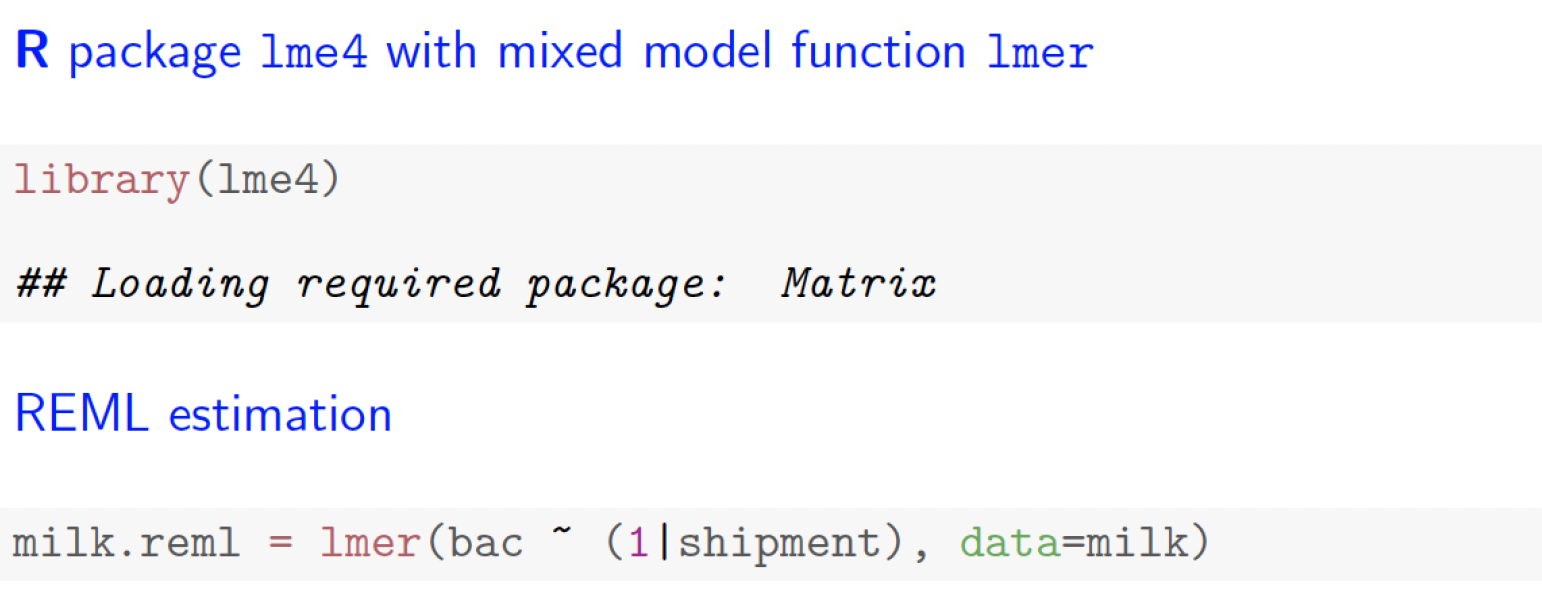
\includegraphics[scale=0.4]{REML.png}
    \caption{}
    \label{}
\end{figure}\end{center}
\begin{center}\begin{figure}[htb]
    \centering
    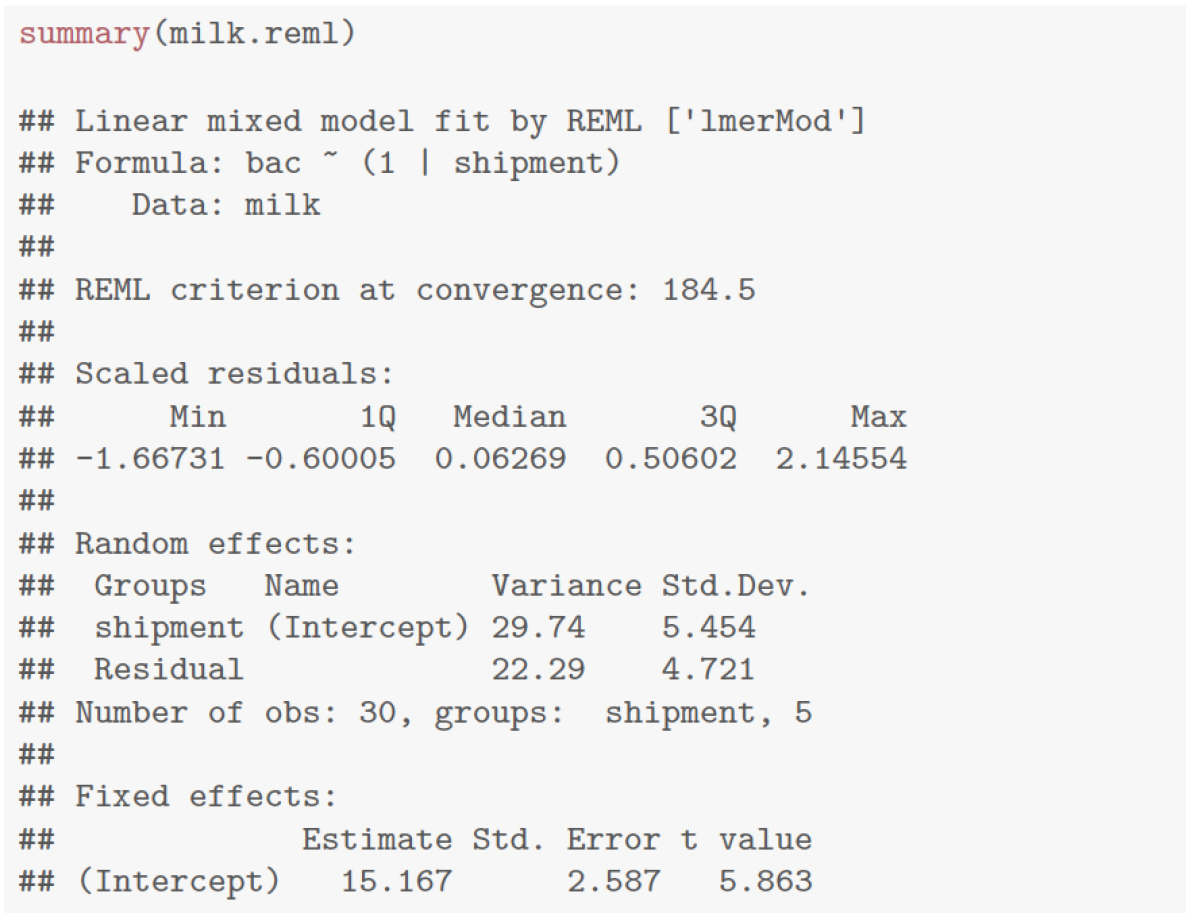
\includegraphics[scale=0.4]{REML2.png}
    \caption{}
    \label{}
\end{figure}\end{center}

- The formula bac (1|shipment) specifies the one-way random effects ANOVA model. As usual, there is an automatically-added intercept (representing $\mu$ ), and the term (1|shipment) represents the random effect term $\alpha_{i}$.\\
- Function Imer uses the REML method, by default. We see that the REML estimates of the variance components are
$$
\widehat{\sigma}_{\alpha}^{2} \approx 29.74 \quad \widehat{\sigma}^{2} \approx 22.29
$$
(The Std.Dev. column simply gives the square roots of these: $\widehat{\sigma}_{\alpha}$ and $\widehat{\sigma}$.)\\
- The only fixed effect is the intercept, $\mu$.\\

\subsection{ML Estimation}

\begin{center}\begin{figure}[htb]
    \centering
    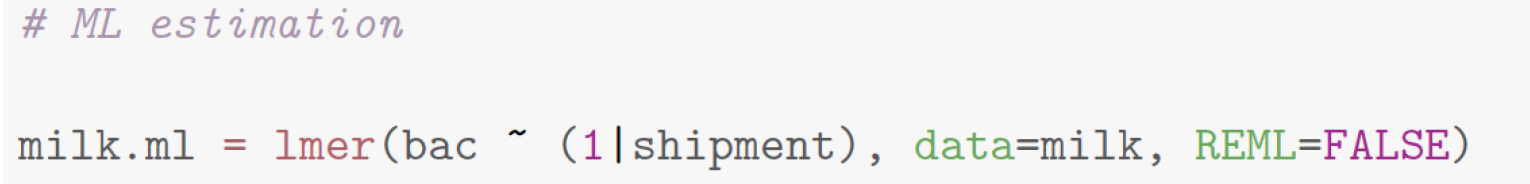
\includegraphics[scale=0.4]{ML Est1}
    \caption{}
    \label{}
\end{figure}\end{center}
\begin{center}\begin{figure}[htb]
    \centering
    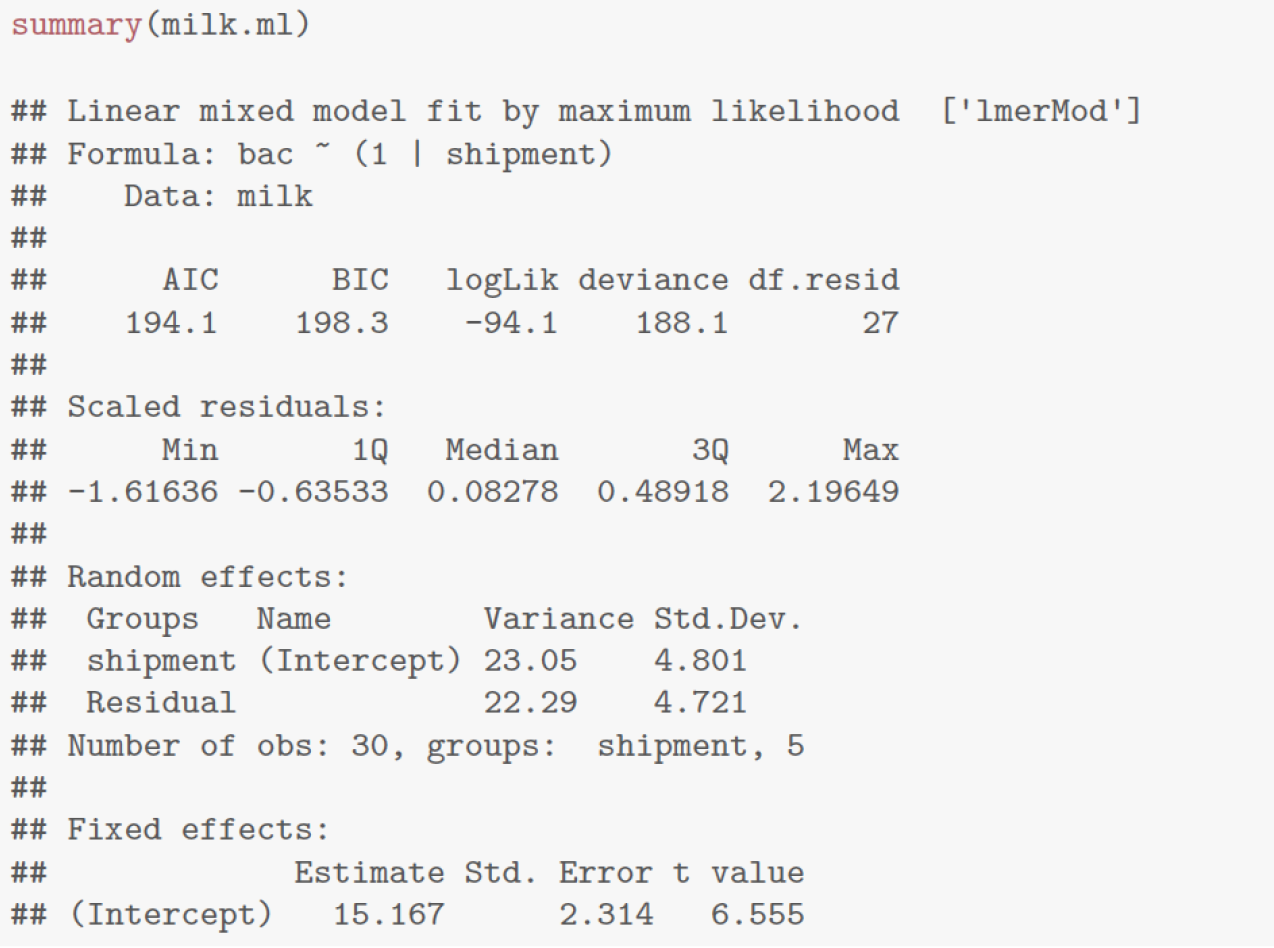
\includegraphics[scale=0.5]{ML Est2}
    \caption{}
    \label{}
\end{figure}\end{center}
- So the MLE for $\sigma_{\alpha}^{2}$ is
$$
\widehat{\sigma}_{\alpha}^{2} \approx 23.05
$$
smaller than the REML estimate 29.74. MLEs for variance components are often biased low.\\
- The estimate listed for $\sigma^{2}$ is apparently not the MLE, but is still the REML estimate.\\
- In this case, the estimate of $\mu$ has remained unchanged, but its standard error has changed.\\

\subsection{ Testing and Confidence Intervals}
- For the fixed effects (in $\beta$ ), likelihood ratio tests are available. (For this to work, the variance components should be estimated with MLE, not REML.)\\
(These LRTs are sometimes unreliable, so a parametric bootstrap approach can be used - later.)\\
- The methods of generalized least squares ( $F$-tests and $t$-tests) could alternatively be used (though this would ignore the additional uncertainty of replacing $\mathbf{D}$ with $\widehat{\mathbf{D}}$ ).\\
- There are also confidence intervals for fixed effect parameters based on the Wald approach or (perhaps more reliably) on profile likelihood.\\

\subsection{ Testing the Random Effect Variance}
- For the random effects, the null hypothesis is usually that a variance component equals zero.\\
- For technical reasons, the usual chi-square approximation in the LRT often fails to be adequate (most often leading to a test that is too conservative).\\
- An improvement is to use the parametric bootstrap to perform the LRT (see example later).\\
- Methods based on ANOVA are also available, and can be useful in single-factor or balanced cases.\\
- Profile likelihood confidence intervals for variance components can be computed (but may have problems, as the LRT does).\\



\subsection{Parametric Bootstrap}

The parametric bootstrap may be more accurate in small samples. Here are the steps:\\
1. Compute the LR statistics for the null and alternative models\\
2. Generate data under the null hypothesis model\\
3. Fit the null and alternative model for the generated data\\
4. Compute the LR statistic\\
5. Repeat steps 2 to 4 many times\\
6. Find the Bootstrap probability of exceeding the observed LR value\\
















































































































































































\end{document}